% Compilar con xelatex
% Generar rtf con latex2rtf TFGandrea.tex
% apt-get install texlive texlive-lang-spanish texlive-latex-extra texlive-xetex
\documentclass[a4paper,11pt]{scrbook} % tipo del documento: scrbook, amsbook, book, article

%% Paquetes necesarios para la correcta compilación
%\usepackage[latin1]{inputenc} % usar caracteres raros como ñ á é ¿ etc
\usepackage[spanish]{babel} % español

\usepackage{array} %Use the package array and specify the font just after the \begin{tabular}
\usepackage[
	pdfauthor={Andrea Ubis Moreno},
	pdftitle={Burbujas económicas - Trabajo Fin de Grado},
	pdfsubject={Burbujas económicas},
	pdfkeywords={Comportamiento de manada, exuberancia irracional, colapso, crisis financiera, burbuja, especulación, Herding, irrational exhuberance, crash, financial crisis, bubbles, speculation},
	pdfproducer={XeLateX with hyperref},
	pdfcreator={Xelatex}
]{hyperref} % Usar enlaces en bibliografía, web, etc. y metadata
\usepackage{lmodern,textcomp} % permite usar €
\usepackage{graphicx} % Usa gráficos desde pdf
\usepackage{pdfpages} % Añade páginas en pdf

\usepackage{amsmath} % Use gather in math formulas

\usepackage{tocbibind} % Add bibliography to table of contents

\usepackage[top=2.5cm, bottom=2.5cm, left=3cm, right=2.5cm]{geometry} % Cambia los margenes

\usepackage{chngcntr} % No reiniciar el contador de figuras o tablas en capítulos
\counterwithout{figure}{chapter}
\counterwithout{table}{chapter}

%% Putas fuentes del señor decano
\usepackage{fontspec} % Cambiar fuente por defecto
\setmainfont{Liberation Sans}
\usepackage{setspace} % Interlineado (line spacing)
\setstretch{1.15}
\makeatletter
\renewcommand\huge{\@setfontsize\huge{24pt}{24}}
\renewcommand\Large{\@setfontsize\Large{18pt}{18}}
\renewcommand\large{\@setfontsize\large{14pt}{14}}
\makeatother
\setkomafont{chapter}{\huge\mdseries}
\setkomafont{section}{\Large\mdseries}
\setkomafont{subsection}{\large\mdseries}


%% Información sin relevancia
\title{Burbujas económicas - Trabajo Fin de Grado}
\author{Andrea Ubis Moreno}


            
%%%%%%%%%%%%%%%%%%%%%%%%%%%%%%%%%%%%%%%%%%%%%%%%%%%%%%%%%%%%
%% Empieza el documento                                   %%
%%%%%%%%%%%%%%%%%%%%%%%%%%%%%%%%%%%%%%%%%%%%%%%%%%%%%%%%%%%%
\begin{document}

\pagenumbering{roman}
%% Añadimos la portada externa

\includepdf{portada/portada}

%\cleardoublepage %Dos páginas en blanco

\section*{Copyright}
El poseedor de esta obra tiene permiso para copiar, distribuir y/o modificar todos los contenidos de este documento bajo los términos de la licencia \emph{Creative Commons Attribution-NonCommercial-ShareAlike 4.0}. Es posible encontrar una copia de esta licencia en \url{http://creativecommons.org/licenses/by-nc-sa/4.0/}

En esta obra se han utilizado imágenes de dominio público o licenciadas bajo Creative Commons. En las imágenes de terceros, se ha reconocido su autoría según se indicaba en donde fueron recogidas.

Obra realizada por \emph{Dña. Andrea Ubis Moreno} con colaboración del \emph{Dr. Juan Pintos Clapés}.

Copias de esta obra y el texto fuente de la misma se pueden encontrar en \url{https://github.com/}


%%%%%%%%%%%%%%%%%%%%%%%%%%%%%%%%%%%%%%%%%%%%%%%%%%%%%%%%%%%%
%% Comenzamos                                             %%
\frontmatter                                              %%
%%%%%%%%%%%%%%%%%%%%%%%%%%%%%%%%%%%%%%%%%%%%%%%%%%%%%%%%%%%%


\section*{Resumen}

El presente trabajo pretende, mediante un enfoque histórico, explicar la
naturaleza de las burbujas a través de perspectivas alternativas sobre
el significado económico y el origen de las mismas y más concretamente
de tres de ellas clásicas.

A lo largo del documento se examinan cuestiones relacionadas con el
pensamiento científico que rodea a las burbujas, ilustrando las
dificultades de coordinación entre las diferentes corrientes de
pensamiento que pueden derivar de cada una de ellas.

\section*{Palabras clave}

Comportamiento de manada, exuberancia irracional, colapso, crisis financiera, burbuja, especulación.

\section*{Abstract}

This essay will use a historical focus to explain the nature of economic bubbles using unconventional alternative perspectives regarding their origins and significance.  In particular, three classical examples perspectives will be examined.

The document will study various theories about bubbles, highlighting the difficulties in coordinating the many currents of thought which derive from these theories.

\section*{Key words}

Herding, irrational exhuberance, crash, financial crisis, bubbles, speculation.





\tableofcontents

\listoffigures
\listoftables

\chapter{Introducción}

\section{Tema a tratar, justificación y objetivos}
El tema elegido para el desarrollo del trabajo fin de grado de
administración y dirección de empresas ha sido \emph{Burbujas económicas},
justificado por mi interés en la rama de historia económica.

En el año 2.008, momento en el que me encontraba cursando la diplomatura
de ciencias empresariales en la Universidad de La Rioja, se comenzó a
escuchar el término \emph{burbuja económica}, más concretamente la burbuja
inmobiliaria que estaban sufriendo multitud de países, entre ellos
España. Muchos fueron los artículos leídos por aquel entonces acerca de
hipotecas subprime o tipos de interés entre otros muchos conceptos que
conciernen a tan complejo término. 

Por lo tanto, el presente trabajo tiene como principal objetivo dar luz
a uno de los ámbitos más ambiguos y controvertidos de la Ciencia
Económica: \emph{las burbujas económicas}. Para ello, se explicará qué son, se analizará la existencia de éstas y se ofrecerá una visión histórica a través de diferentes ejemplos surgidos a lo largo de los tiempos. Se investigarán diversas teorías sobre las mismas y se plantearán sus efectos en el panorama económico de la época. 

\section{Estructura y metodología}
La estructura del proyecto consta de cuatro capítulos con los siguientes
contenidos.

En el capítulo uno, se explicará la situación en la que el precio de un
bien o un activo, dentro de un mercado específico, se encuentra por
encima de su precio \emph{normal}. Se dará una visión histórica
recorriendo las diferentes burbujas relevantes surgidas a lo largo del
tiempo. El concepto de burbuja económica quedará ilustrado por las
primeras teorías económicas psicológicas sobre las mismas, que se basan
en factores humanos, sociales, de comportamiento y expectativas. Por
otro lado, se ofrecerán los argumentos de los autores que consideran la
inexistencia de las burbujas económicas. También se razonará si éstas
pueden generar redistribución de la riqueza o por el contrario
perjudica gravemente la economía. 

En el segundo capítulo, se describe la que posiblemente sea la primera
burbuja económica de la historia, la tulipomanía, surgida en los Países
Bajos en 1.637. A lo largo del capítulo, se da una amplia visión del
contexto histórico holandés en el que se desarrolló dicha burbuja, se
analizan las fases de ésta, se nombran diferentes fuentes de las que se
pueden obtener datos sobre los precios de los tulipanes en la época y
por último se estudia la influencia de las redes sociales del momento y
cómo afectó al fenómeno especulativo. 

En el Capítulo 3, se expone la burbuja de la Compañía del Mississippi
desarrollada en Francia a lo largo del siglo XVIII. Se explica la
implantación del revolucionario sistema económico financiero
desarrollado por el escocés John Law. Se analizará como afectó este
método a la deuda del país, como devastó el sistema financiero francés
desarrollando una burbuja económica y se dan diferentes conclusiones
de autores. 

En el Capítulo 4, se estudia la burbuja económica de la Compañía de los
Mares del Sur dada en Inglaterra en el siglo XVIII. Se da una visión
del marco histórico inglés y su paralelismo con la burbuja de la
Compañía del Mississippi, de la que le separan escasos años de
diferencia. 

Por último, se han extraído una serie de conclusiones alcanzadas por los
autores mencionados a lo largo del proyecto y las cuales se han ido
encuadrando dentro del tema a tratar. Además, a lo largo del trabajo se
han ido incluyendo conclusiones que, de forma parcial, se presentan en
algunos epígrafes.

La metodología llevada a cabo para conceptualizar el tema a desarrollar
a lo largo del proyecto ha sido la recopilación de artículos de
investigación, lectura y comprensión de textos para poder ofrecer la
mayor rigurosidad posible. 



%%%%%%%%%%%%%%%%%%%%%%%%%%%%%%%%%%%%%%%%%%%%%%%%%%%%%%%%%%%%
%% Capitulos                                              %%
\mainmatter                                               %%
%%%%%%%%%%%%%%%%%%%%%%%%%%%%%%%%%%%%%%%%%%%%%%%%%%%%%%%%%%%%

\chapter{¿Qué es una burbuja económica?}
Para poder dar una correcta definición de qué es una burbuja económica, se han de tener claros dos conceptos fundamentales en economía: el valor y la sobrevaloración de los precios de un bien o servicio. 
\section{El valor y la sobrevaloración} 
El valor es un concepto subjetivo de difícil definición, ya que cada individuo tiene diferentes perspectivas según la postura en la que se encuentre. 

En primer lugar, hay que añadir que es una variable que influye a la hora de llevar a cabo transacciones donde también hay involucrados múltiples agentes de toda la cadena productiva y comercial, como son los propietarios, los proveedores, las empresas y los vendedores. 

Se plantea una cuestión, \emph{¿Cuál es el significado de valor en el contexto de los negocios?} Según la Real Academia de la Lengua Española define valor como \emph{el grado de utilidad o aptitud de las cosas, para satisfacer las necesidades o  proporcionar bienestar o deleite}. Por otro lado, el conocido autor en materia económica Michael Porter (1.980), define el valor como \emph{una cadena vertical que abarca desde los proveedores de recursos hasta los compradores finales teniendo en cuenta a las empresas y sus servicios. El valor se crea a lo largo de esta cadena sufriendo variaciones debidas a los diferentes agentes. Estos agentes son los proveedores, las empresas y los compradores}	\footnote{Fuente: Porter (1.996)} . Esta cadena se puede observar en la Figura \ref{fig:Cadena de agentes}.

\begin{figure}[!h]
	\caption{Cadena de agentes}
	\centering 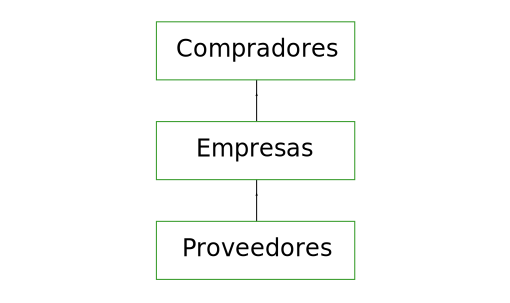
\includegraphics[width=150mm]{capitulos/graficos/cadenaAgentes} 
	\label{fig:Cadena de agentes} 
	
		\footnotesize
		Fuente: Brandenburguer, \& Harbone, (1.996)


\end{figure}

El valor añadido viene definido por el autor Brandenburguer (1.996) como, \emph{el valor creado a lo largo del proceso. Desde los proveedores hasta los compradores, teniendo en cuenta la cantidad y el precio que estos están dispuestos a adquirir o a pagar respectivamente, no sólo por un producto o servicio que cubra las necesidades, si no por un producto que aporte algún factor añadido} \footnote{Fuente: Brandenburguer, \& Harbone, (1.996)} 

Continuando la teoría de Brandenburguer y Harbone (1.996), en un modelo simplificado, el valor viene definido por la voluntad de pago del comprador y por el coste de oportunidad del vendedor, siguiendo una ecuación: 

\begin{gather*}
    Valor = voluntad - coste
\end{gather*}

Como se mencionó al comienzo del epígrafe, la definición de valor parece abstracta y en algunos contextos lo es. También es complicado realizar un cálculo por lo que se puede plantear otra cuestión, \emph{¿Cómo se determina el valor apropiado para cada agente de la cadena?} Se puede observar de una manera rápida y visual gracias a la Figura \ref{fig:Cadena de valor}.

\begin{figure}[!h] 
\caption{Cadena de valor} 
\centering \includegraphics[width=150mm]{capitulos/graficos/cadenaValor} 
\label{fig:Cadena de valor} 

	\footnotesize
	Fuente: Brandenburguer, \& Harbone, (1.996)

\end{figure}

Por lo tanto, se puede concluir que debido a la existencia de multitud de oferta, la diversidad de compradores tiene varias opciones de compra. De este modo, tiene que existir congruencia entre compradores y vendedores llegando a alcanzar un trato positivo para ambas partes y de este modo alcanzar el equilibrio de mercado.

Una vez queda explicado el valor, frente al precio ordinario de un bien o servicio, se ha de plantear otra cuestión, \emph{¿Cómo se puede saber si un bien se encuentra sobrevalorado por los consumidores?} \emph{El valor} es un concepto abstracto y propio de cada individuo tal y como se ha mencionado. Alcanzar su conocimiento de una forma directa con instrumentos económicos, parece un hecho imposible en la actualidad. Por ello, resulta más sencillo realizar estimaciones con precios reales aplicando dos métodos fundamentales establecidos por los autores Brandenburguer y Harbone (1.996) y que tan sólo se mencionaran debido a su complejidad. Por un lado el método de ratios que compara los precios de un bien o servicio con respecto a otro indicador. El resultado se contrasta con otro valor que el mercado lo encasilla en fase de normalidad. Un ejemplo es el ratio del PER. Y por otro lado, el método de residuos de un modelo \emph{X} que consiste en explicar los precios a través de un modelo econométrico teniendo en cuenta variables clásicas tales como el carácter demográfico, tipos de interés, etc. Éste último es un método más costoso que el anterior.

Una vez explicados estos dos conceptos abstractos, se puede comenzar a dar forma a la definición de burbuja económica. 

\section{¿Qué es una burbuja económica?}

El concepto de burbuja económica no está exento de cierta ambigüedad. Si bien existe un razonable acuerdo en asociarlo con un intenso y prolongado aumento en el precio de un activo, seguido por una abrupta y rápida caída del mismo; no hay consenso acerca de cuáles son las causas que provocan la burbuja ni sobre cuál debe ser su definición única y precisa. En particular, no existen límites preestablecidos para determinar hasta qué punto el precio de un activo debe subir y cómo debe subir para que se considere un caso de burbuja económica. 

A este fenómeno en sus orígenes se le denominaba  \emph{manía}. La palabra manía, tiene en cuenta a los individuos o agentes que se introducen en el mercado en el momento en el que éste se encuentra más exaltado por los inversionistas. En ese momento, la venta parcial o total de los activos tiene el fin de comprar más activos para lucrarse en un futuro, es decir, lo que hoy llamaríamos un \emph{proceso especulativo}. La manía concluye cuando algunos individuos o agentes venden los activos al percatarse de que los precios no podrán mantener esa trayectoria ascendente. La caída de precios se produce por el descenso de demanda.

La primera de ellas surgió en Holanda en 1.637 en el mercado del tulipán. Algunos de los tulipanes, como se verá a lo largo del capítulo dos, alcanzaron precios desorbitados. El concepto de esta manía, refleja el hecho de que los individuos adquirían tulipanes a un precio muy alto con la expectativa de venderlos a un precio aún más alto a otro individuo o agente que tuviese una mayor expectativa sobre la evolución futura de los precios. La palabra manía tiene en cuenta también el hecho de que la venta parcial o total de estos tulipanes tiene como fin la compra de más tulipanes para poder cobrar beneficios adicionales, es decir, para llevar a cabo un proceso especulativo. Esta manía finalizó cuando algunos individuos vendieron sus tulipanes ya que creyeron que los precios no podrían mantenerse tan elevados. 

Como se va a poder comprobar a lo largo del presente capítulo, una burbuja económica puede aparecer prácticamente en cualquier lugar del mundo. Por ejemplo han surgido en países como Argentina, Australia, China, Estados Unidos, España, Holanda, Irlanda, Japón, Rumanía, Zimbabwe, etc. También se puede destacar la variedad de materias primas, bienes o servicios que han sido víctima de este fenómeno como por ejemplo los tulipanes, las acciones, el uranio, el rodio, el trigo, los inmuebles, etc. 

Los efectos y resultados a posteriori de la burbuja económica, también pueden variar dependiendo de diferentes factores. Sin embargo, existe una clara evidencia empírica de que las burbujas económicas generan una redistribución de la riqueza entre los diversos agentes de la economía. Es evidente que puede dañar la economía, pero también puede generar una fuerte desviación temporal en cuanto a la tendencia del precio se refiere, o por el contrario incluso en algunos casos podría beneficiar a la economía, como se comprobará a lo largo del presente capítulo, aunque este último aspecto causa controversia en sí mismo. Se pueden demostrar estos hechos beneficiosos con los ejemplos de expansión y proliferación de Internet durante la burbuja punto com, o el Crack de 1.929 en Estados Unidos entre otros, desarrollados a continuación. Estos efectos serán expuestos más adelante.

Retomando la intención de dar una definición apropiada al término burbuja económica no se puede pasar por alto la analogía presentada por uno de los autores principales en la materia, Van Horne (1.985). Este autor presenta un paralelismo entre una burbuja y un globo. De este modo se puede comprender de una forma visual cómo se desarrollan las burbujas. Defiende que una burbuja económica es como un globo que se infla progresivamente y puede realizarlo de dos formas diferentes. El primer caso, es introducir el aire gradualmente impidiendo que éste se desprenda precipitadamente. Y la segunda opción, es que el aire se introduzca rápidamente y haya más probabilidades de que se produzca un pinchazo en el globo, lo que provocaría la explosión de éste y por lo tanto, retomando la burbuja económica, que los precios aumenten repentinamente hasta llegar a un punto en que éstos han de descender. Esto puede suceder de una forma repentina o paulatinamente. Obviamente las consecuencias son muy diferentes según se desarrolle cada caso
.

Llegados a este punto del capítulo, se puede afirmar que la definición teórica que más se asemeja al término de burbuja económica es la de DeMarzo (2.007): \emph{Se define una situación de burbuja en el momento en el que existe un precio de mercado de un activo que es superior a su valor fundamental, siendo el valor fundamental el valor presente de los pagos futuros}. 

\section{Breve cronología de las burbujas económicas más importantes a lo largo de la historia} 
A continuación se van a narrar brevemente algunas de las burbujas económicas históricas más relevantes.
\subsection{La tulipomanía} 
Esta burbuja histórica clásica, desarrollada en profundidad en el capítulo dos, tiene como pieza principal los tulipanes. Esta planta fue importada a Holanda a finales del siglo XVI y no tardó en convertirse rápidamente en un bien caro pero accesible antes de la manía. La locura se desató en el momento en el que algunos tulipanes comenzaron a adquirir diferentes colores en una misma flor y se comenzaron a \emph{sobrevalorar} estos bulbos extremadamente raros \footnote{Se dará explicación detallada acerca de estos tipos de tulipanes en el capítulo dos.} y bellos.

En un principio eran sólo comerciantes los que especularon con el precio futuro de los tulipanes, comprando así, grandes cantidades de éstos mismos con antelación para la temporada siguiente. Pero a medida que los precios aumentaron, gran parte de la población quería ser partícipe introduciéndose en el mercado y empezando a especular con tulipanes. 

\begin{figure}[!h] 
\caption{Nivel de precios de la Tulipomanía} 
\centering 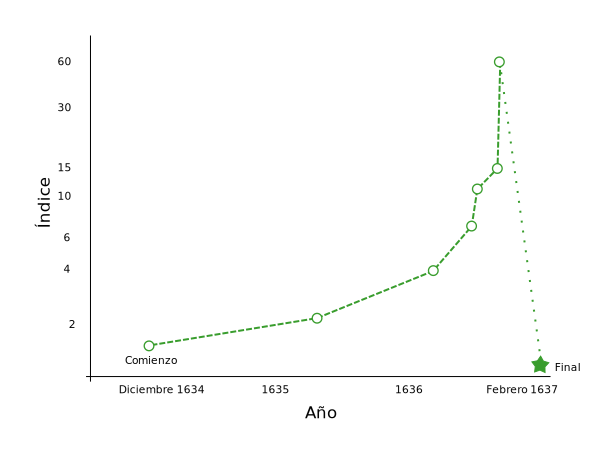
\includegraphics[width=150mm]{capitulos/graficos/TulipBubble} 
\label{fig:Nivel de precios de la Tulipomanía} 

	\footnotesize
	Fuente: Eliot Wave International (1.999)

\end{figure}

Como se puede apreciar en la Figura \ref{fig:Nivel de precios de la Tulipomanía}, el punto álgido de la burbuja tuvo lugar a principios de 1.637, cuando tan solo un bulbo de tulipán \emph{raro}, se vendía por una cantidad equivalente al precio del castillo de un noble. La manía, sumergida en un continuo circuito de retroalimentación negativa, provocó que la deflación del bulbo creciese a un ritmo cada vez más rápido. En escasos días, el pánico reinaba en Holanda y los precios se desvanecieron. Este episodio fue seguido por una severa disminución de la actividad económica de la que se necesitaron muchos años para conseguir la completa recuperación.

\subsection{La Compañía del Mississippi} 

La burbuja de la Compañía del Mississipi será analizada en profundidad en el capítulo tres. 

Se trata de una burbuja económica que se dio en Francia a principios del siglo XVIII y que se desarrolló en paralelo con la burbuja de la Compañía de los Mares del sur en Gran Bretaña. El cerebro que se escondía tras la burbuja del Mississippi era John Law, un financiero escocés que ascendió a los escalones superiores de la hacienda pública francesa a través de su amistad con el Archiduque de Felipe II de Orléans.

Law se convirtió en el primer asesor financiero del gobierno francés y utilizó a este para poder instaurar un banco con la autoridad suficiente como para emitir \emph{dinero papel}; y en segundo lugar, otorgando un monopolio en el mercado a La Compañía del Mississippi. De este modo, a principios de 1.719, esta Compañía absorbió gran cantidad de compañías mercantiles importantes renombrándose \emph{La Compañía de las Indias}. En julio de ese mismo año, la Compañía adoptó el derecho de cobrar todos los impuestos indirectos franceses y en octubre de 1.719 se hizo cargo de la recaudación de impuestos directos.

\begin{figure}[!h] 
\caption{Precio de las acciones de la Compañía del Mississippi 1.719 - 1.720} 
\centering \includegraphics[width=150mm]{capitulos/graficos/preciosAccionesIndias} 
\label{fig:PrecioAccionesCompaniaMississippi} 

	\footnotesize
	Fuente: Thornton, H (2.010)

\end{figure}

Como se puede comprobar en la Figura \ref{fig:PrecioAccionesCompaniaMississippi} , la explosiva demanda de acciones de la Compañía de las Indias, provocó que la cantidad total de dinero papel que el banco expedía, aumentase en un 186 por ciento en un año. Pero en enero de 1.720, las acciones de la Compañía comenzaron a caer en picado ya que algunos inversores decidieron retomar el antiguo sistema de monedas de oro y plata. Las acciones de la Compañía, se devaluaron y el dinero papel lo hizo en mayor medida alcanzando el 50 por ciento en mayo de 1.720 y creando pánico entre los inversores. Estos inversores se arruinaron y a finales de 1.720, John Law fue visto como un estafador y escapó de Francia. El colapso del banco nacional y la Compañía de las Indias coincidió con el estallido de la burbuja de los Mares del Sur de Gran Bretaña.

\subsection{La Compañía de los Mares del Sur}  

El estudio en profundidad de esta burbuja económica se desarrollará en el capítulo cuatro.

En el año 1.711, en la ciudad de Londres, se fundó la Compañía de los Mares del Sur, la cual ayudó a restaurar la fe en la solvencia del gobierno mediante la compra de diez millones de libras en bonos del gobierno. La Compañía, recibió el monopolio del comercio inglés de los Mares del Sur. Había un gran entusiasmo acerca de los beneficios que se podían alcanzar desarrollando un comercio con América, ya que la Compañía siempre se las arregló para tener una buena propaganda positiva y sus perspectivas de comercio mejoraron cuando Gran Bretaña puso fin a la guerra con España y México. La compañía tenía el favor distintivo del gobierno y tanto los inversionistas como el pueblo creían que existían riquezas potenciales que se llevarían a cabo con en el nuevo comercio de oro, plata, algodón y lana en América. En 1.720, se propusieron aumentar la reputación de la Compañía ofreciéndose a financiar la totalidad de la deuda nacional, que ascendía a 31 millones de libras. Este hecho inició la especulación sobre el precio de las acciones. 

Como se puede observar en la Figura \ref{fig:PrecioAccionesMaresSur}, el 7 de abril tras ser publicado un proyecto de ley en el Parlamento, el precio de las acciones aumentaron rápidamente de 130 a 300 libras. Con el tiempo, el precio de las acciones aumentó hasta alcanzar las 1.000 libras. Llegado a ese punto, el precio de las acciones no tenía concordancia con la situación real de la empresa y los directores, y demás individuos influyentes, decidieron vender sus participaciones durante el verano.

\begin{figure}[!h] 
\caption{Precio de las acciones de la Compañía de los Mares del Sur 1.717 - 1.722} 
\centering 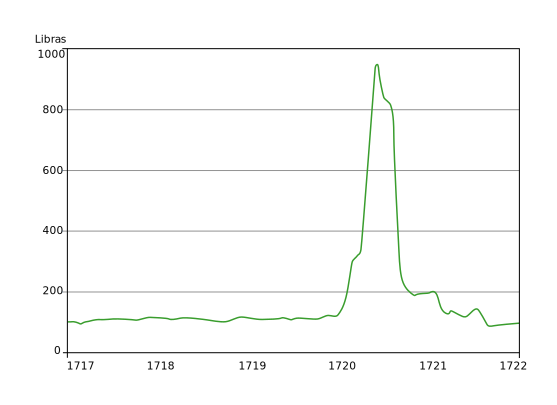
\includegraphics[width=150mm]{capitulos/graficos/SouthSeaStockPrice} 
\label{fig:PrecioAccionesMaresSur} 

	\footnotesize
	Fuente: L. Neal (1.990)

\end{figure}

La noticia llegó a oídos de la multitud y el pánico se instaló en el pueblo, provocando que el precio se derrumbase. Entre los grandes perjudicados de la burbuja de los Mares del Sur se encuentra Isaac Newton, quien exclamó: \emph{Puedo calcular los movimientos de los cuerpos celestes, pero no la locura de la gente}. 

Se trata de una historia muy similar a la de la Compañía de los Mares del Sur, que ocurrió en el mismo período de tiempo en Francia. Durante este período de tiempo hubo casos masivos similares de empresas que comenzaban a prometer grandes recompensas y en algunas ocasiones se trataba de fraudes donde los propietarios se quedaban con el dinero de las inversiones.


\subsection{La manía del ferrocarril}  

Al mismo tiempo que se gestaba la Revolución Industrial en Gran Bretaña, surgió la necesidad de crear un gran sistema de transporte tanto para la industria como para la población. Así, el ferrocarril parecía una necesidad imperiosa. En un principio, cientos de empresas ofrecieron presupuestos al Parlamento para que éste los aprobase, un total de 272 fueron aptos. Finalmente, se tuvieron en cuenta todos los proyectos de todas las empresas ferroviarias y se creó una propuesta global de construcción de 15.300 kilómetros de vía. Por otro lado, en el país, las familias con poder adquisitivo medio iban en aumento al mismo tiempo que una gran parte de la población sabía leer y escribir. Este sector de la población, también poseía ahorros acumulados y se sentían dispuestos a invertir. Además, el Banco de Inglaterra redujo los tipos de interés y el gobierno promovió en gran medida los proyectos ferroviarios.

Seis mil individuos se convirtieron en inversores del ferrocarril haciéndose con un gran número de acciones pagando un depósito. La Manía del ferrocarril fue víctima de una verdadera campaña publicitaria por parte del gobierno y de algunas empresas poco solventes. En el año 1.845, la inviabilidad de muchos proyectos se hizo evidente. El Banco de Inglaterra, no tardó en elevar los tipos de interés a finales de ese año y muchas empresas se quedaron sin fondos. Las perspectivas de rentabilidad de las inversiones desaparecieron.

\begin{figure}[!h] 
\caption{La Railmania} 
\centering 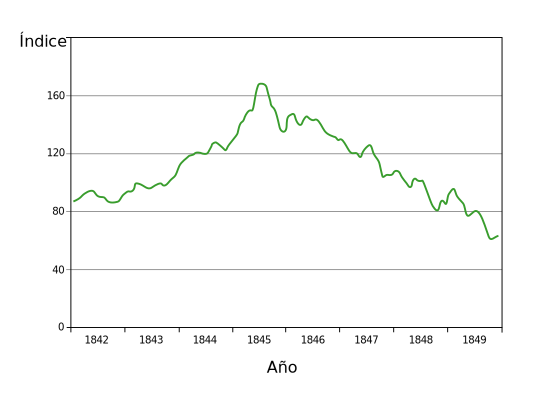
\includegraphics[width=150mm]{capitulos/graficos/LaRailmania} 
\label{fig:La Railmania} 

	\footnotesize
	Fuente: Global Financial Data, Inc

\end{figure}

A principios de 1.850 sobrevivieron las principales compañías ferroviarias. Sin embargo, en este caso no hubo un efecto tan relevante en la población tras el estallido de la burbuja como algunos autores señalan. Entre ellos, Wolmar, (2.007). El sistema ferroviario británico se expandió enormemente durante el período de euforia inversionista debido al frenesí especulativo que atrajo importantes cantidades de capital privado que eran necesarios para la construcción del ferrocarril, además de que los bancos estaban dispuestos a prestar.

Un total de 10.000 kilómetros se construyeron como resultado de proyectos autorizados entre 1.844 y 1.846. Es interesante compararlo con la red ferroviaria moderna del Reino Unido, que abarca un total de 34.000 kilómetros. Este hecho da una idea de la importante construcción realizada en un corto período de tiempo.

\subsection{El Crack del 29}  

En cuanto a los mercados modernos, se tiene que mencionar el gran mercado alcista de los Estados Unidos que se derrumbó en 1.929. Está considerada como una de las mayores burbujas bursátiles de todos los tiempos.

La explicación más aceptada de lo ocurrido en el mercado de valores de Estados Unidos es la dada por Galbraith (1.954), en la que señala que la burbuja se fue gestando durante el rápido crecimiento y expansión del crédito en forma de préstamos que los inversores no pagaban. Sin embargo, hay otros estudios que afirman el hecho de la inexistencia de burbuja económica durante este período, ratificando que los precios de las acciones reflejan los valores fundamentales de acuerdo con los estudios econométricos, en este caso, el autor relevante que defiende esta postura es Hamilton (1.986). Una versión revisada y completa de este estudio apunta a una combinación de factores generadores de la burbuja económica que no eran tan sólo los mencionados por Galbraith. Estos factores no pueden ser detectados con los datos econométricos ya que el periodo de tiempo transcurrido fue muy corto según establece White (1.990).

A partir de 1.928, la especulación en el mercado de valores se convirtió en un pasatiempo nacional. De 1.922 a 1.929, el PIB creció a una tasa anual del 4,7 por ciento y el desempleo descendió un 3,7 por ciento. Grandes condiciones económicas se estaban propiciando. Por ejemplo la aparición de las grandes empresas comerciales e industriales, las economías a escala y la gestión moderna. Las empresas emitían acciones para financiar nuevas naves y equipos. Los bancos comerciales comenzaron a dedicarse a la banca de inversión creando filiales. El número de afiliados creció de 10 a 114 entre 1.922 y 1.931, según indica Peach (1.941) en su estudio. Gran parte de los nuevos inversores que participaron en el mercado de valores, carecían de experiencia, facilitando así la creación de la burbuja. Entre el 3 de marzo de 1.928 y el 3 de septiembre de 1.929 la participación en los principales valores que cotizaban en Wall Street aumentó del 87 por ciento hasta 434,5 por ciento como según afirma Malkiel (1.973).

\begin{figure}[!h] 
\caption{El crack de 1.929} 
\centering 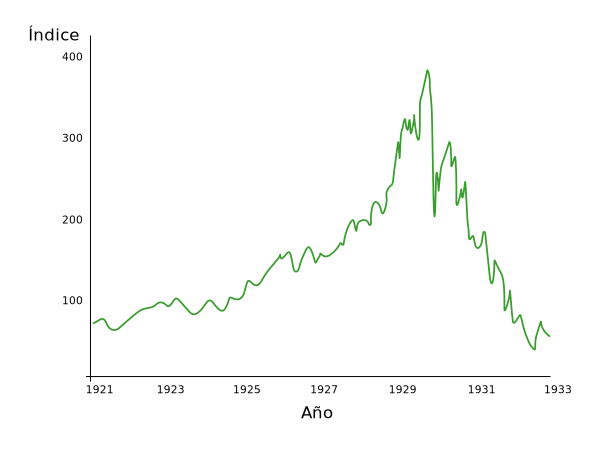
\includegraphics[width=150mm]{capitulos/graficos/1929Bubble} 
\label{fig:El crack de 1.929} 

	\footnotesize
	Fuente: Elaboración propia a partir de los datos recuperados en Dow Jones Industrials (2.012)

\end{figure}

En el mes de septiembre del año 1.929, y tal como se puede apreciar en la Figura\ref{fig:El crack de 1.929}, hubo más días malos que buenos. Aun así, los banqueros y los funcionarios del gobierno aseguraron al país que no había motivo de preocupación. El 21 de octubre de 1.929, todo estaba preparado para el colapso del mercado. Las caídas de las cotizaciones bursátiles llevaron a exigir más garantías a los clientes que habían comprado acciones con dinero prestado. Estos clientes se vieron obligados a vender sus pertenencias para hacer frente a la deuda adquirida en el pasado. Esta caída de los precios realizó un ajuste de los márgenes de dinero prestados y una ola vendedora de acciones. 

El 24 de octubre de 1.929, más tarde llamado \emph{Jueves Negro}, muchas de las acciones vieron reducidos sus precios en un 25 por ciento durante dos horas. Al día siguiente, el presidente Herbert Hoover lanzó un mensaje al pueblo en el que decía: \emph{El negocio fundamental del país, se encuentra sobre una base sólida y próspera}.

El martes, 29 de octubre 1.929, se considera como uno de los días más catastróficos de la historia de la Bolsa de Valores de Nueva York. La caída de la bolsa fue seguida por una intensa y devastadora depresión, una de las más importantes en la historia del país. El estallido sucedió en sí, debido a las políticas llevadas a cabo, que como consecuencia, elevaron las tasas de interés para castigar a los especuladores.

En contraposición a la idea de que el Crack del 29 fue una burbuja económica, se encuentra la opinión de Bierman Jr (1.991), quien defiende que las acciones no fueron demasiado caras durante el año 1.929 debido a que parecía que la economía seguía una dinámica próspera.

\subsection{La burbuja económica de Japón}  

Durante la década de los 80, Japón comenzó a crecer económicamente durante un largo periodo de tiempo y mantuvo estable la inflación con la excepción del precio de los activos inmobiliarios, que aumentaron rápidamente.

Del año 1.955 hasta 1.990, el valor de los inmuebles japoneses aumentó más de 75 veces, situando así el valor total de todos los bienes mobiliarios, cerca de los 20 billones de dólares, el equivalente a más del 20 por ciento de la riqueza del mundo, según confirma Malkiel (1.973).

\begin{figure}[!h] 
\caption{Precio de las acciones de la Burbuja Japonesa} 
\centering 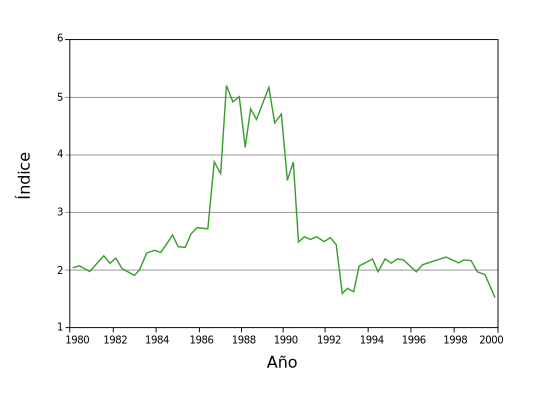
\includegraphics[width=150mm]{capitulos/graficos/JapaneseStockMarketBubble} 
\label{fig:Precio de las acciones de la Burbuja Japonesa} 

	\footnotesize
	Fuente: Estimaciones del banco Morgan Stanley

\end{figure}

Como se puede observar en la Figura \ref{fig:Precio de las acciones de la Burbuja Japonesa}, la burbuja económica se sitúa entre 1.987 y 1.990. Fue entonces cuando los precios de acciones, los precios de los terrenos y los precios de los bienes comenzaron a comportarse de una forma diferente a la habitual. El punto más alto, se alcanzó en diciembre de 1.989, cuando las acciones japonesas tuvieron un valor total de mercado de 4 billones de dólares, casi 1,5 veces el valor de todas las acciones de Estados Unidos y cerca del 45 por ciento del mundo.

Las causas del surgimiento de la burbuja económica pueden ser identificadas como factores interconectados que aumentaron las expectativas optimistas de la economía. Según Shiratsuka, (2.003) el comportamiento agresivo de las instituciones financieras, el progreso de la desregulación financiera, la gestión inadecuada del riesgo por parte de las instituciones financieras, la introducción del Acuerdo de Capital, la flexibilización monetaria prolongada, los impuestos y las regulaciones sesgadas, aceleraron la subida de los precios, provocaron un exceso de confianza y euforia y concentraron sus esfuerzos en convertir a Tokio en un centro financiero internacional. 

Un punto fundamental a tener en cuenta, es que los tipos de interés continuaron siendo bajos a pesar de la expansión económica de la época, lo que contribuye al crédito fácil y barato.

Como en otros casos de burbujas económicas, la disminución de la rentabilidad hizo que los agentes revisasen sus expectativas provocando el desplome del mercado de valores y del mercado inmobiliario. El colapso de esta burbuja en Japón, tuvo profundos efectos en el sistema financiero y en la economía japonesa, por lo que debilitó todo el sistema financiero y fue seguida por una severa recesión que duró hasta el siglo siguiente. 

Hay un cierto paralelismo entre esta burbuja y la de 1.929 en Estados Unidos anteriormente descrita. Principalmente por el extremo colapso que las ciudades vivieron en ambos casos. 

\subsection{La crisis asiática}   

Los países más afectados durante este boom y colapso fueron: Corea del Sur, Filipinas, Indonesia, Malasia y Tailandia.

Entre 1.980 y 1.990, las tasas de interés en las economías desarrolladas, fueron relativamente bajas en comparación con las tasas de interés de las economías en desarrollo de Asia. Este hecho generó un gran flujo de dinero que dio un impulso a las economías regionales de Asia. Los llamados \emph{dragones asiáticos}, lograron tasas de crecimiento del PIB que abarcaban del 12 por ciento al 8 por ciento. Sin embargo, según Krugman (1.994), este crecimiento estaba basado casi puramente en un elevado déficit en sus cuentas corrientes, lo que se tradujo en un endeudamiento externo y a un apalancamiento de la economía debido al riesgo del cambio de divisas. 

Entre 1.995 y 1.996 las exportaciones asiáticas aumentaban a tasas muy elevadas, un 20 por ciento. Se ha de tener en cuenta, que las exportaciones son una variable muy importante en la economía asiática ya que suponen un porcentaje muy alto del PIB nacional. Por ejemplo, en Corea del Sur y Tailandia, el porcentaje asciende al 40 por ciento. En 1.997, las exportaciones comenzaron a descender debido a la revaluación de las diferentes monedas asiáticas, lo que hacía que aumentase la presión entre las monedas, perjudicando así a la asiática y provocando una pérdida de competitividad con el resto de países. Al mismo tiempo, los Estados Unidos se recuperaban de una recesión y comenzaron a subir los tipos de interés. Esto, provocó que las inversiones del país fuesen más atractivas y además se producía una apreciación del dólar. Infinidad de capitales comenzaron a salir y la especulación se volvió pesimista sobre las monedas asiáticas. Todo el proceso de colapso se describe con tan sólo una palabra: \emph{pánico}. 
Se puede comprobar este crecimiento en la Figura \ref{fig:AsianCrisis}.

\begin{figure}[!h] 
\caption{Flujo de capital de los países asiáticos emergentes 1991 - 2010 (Porcentaje según el PIB)} 
\centering 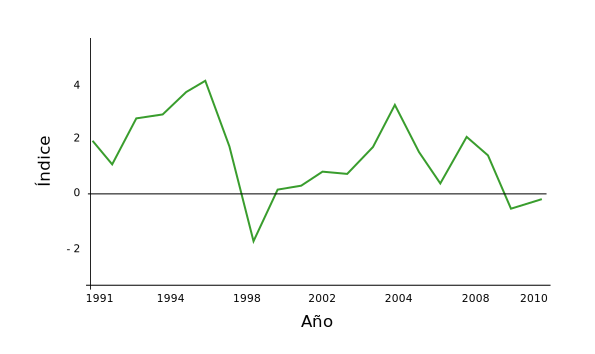
\includegraphics[width=150mm]{capitulos/graficos/AsianCrisis} 
\label{fig:AsianCrisis} 

	\footnotesize
	Fuente: IMF (2.009)

\end{figure}


Al tratarse de un hecho histórico relativamente contemporáneo, todavía hay diferentes puntos de vista sobre las causas de esta crisis, aun así, se va a intentar dar explicación.

El primero, se basa en la teoría desde una perspectiva psicológica. Algunos de los autores relevantes que sostienen esta postura son Radelet y Sachs (1.998), Chang y Velasco (1.999) y Marshall (1.998), y se basan en un cambio de las expectativas debido al contagio regional. Estos autores defienden que, la mayor fuerza causante de esta crisis fue el pánico que surgió entre los inversionistas nacionales e internacionales.

El segundo enfoque, se basa en los fundamentos de los desequilibrios. Como son las distorsiones estructurales, políticas gubernamentales equivocadas y un efecto manada o \emph{herding} \footnote{Concepto definido a lo largo de este capítulo.}.

La tercera visión, está basada en las enormes y rápidas entradas y salidas de capital que fueron devastadoras, junto con los efectos negativos del Yang frente a la moneda extranjera.

Si se mezclan los conceptos de estas tres teorías, se puede apoyar la idea de que una excesiva entrada de dinero va destinada a unos pocos activos, de este modo, infla a éstos por encima de sus valores fundamentales. Si a esto expuesto se le suma que ocurre dentro de una economía que todavía tiene deficiencias estructurales, se puede concluir que estas entradas y salidas monetarias pueden tener unas repercusiones muy graves.

Todo ello se puede apreciar claramente en la Figura \ref{fig:AsianCrisis}.


\subsection{La burbuja punto com}    
Se trata de una de las mayores burbujas del mercado de valores de todos los tiempos que irrumpió en marzo del año 2.000. Más de siete billones de dólares en valores de mercado se evaporaron en tan sólo dos años.

El período viene marcado por la expansión de Internet en la sociedad. Se trataba de una tecnología totalmente revolucionaria que abriría nuevos horizontes. Permitió nuevas posibilidades de negocio, ya que era una novedosa forma de compartir y transmitir información. También proporcionaba nuevas formas de adquirir bienes y servicios. Se le denominó \emph{La Nueva Economía}. Las posibilidades eran ilimitadas, y como tal, se presentaba como un nuevo concepto donde los límites todavía no estaban claros. La retroalimentación positiva comenzó, y en ese momento, los medios de comunicación jugaron un papel muy importante porque supuso un impulso nunca antes visto. Internet no tardó en convertirse en una de las variables más importantes de la vida cotidiana.

Los inversores de capital de riesgo se convirtieron en los principales protagonistas en el inicio del boom. Cuando la primera empresa punto com se hizo popular, el precio de las acciones se disparó automáticamente. Por lo tanto, estos inversores de riesgo modificaron su estrategia habitual y en lugar de centrarse en la viabilidad del proyecto, todos los esfuerzos fueron destinados a que la empresa se hiciese famosa y cobrar así un beneficio rápido y sustancial. En el primer trimestre del año 2.000, 916 empresas invirtieron 15,7 mil millones de dólares en más de mil de las empresas pioneras de Internet, según afirma Malkiel (2.007). Cualquier empresa lo suficientemente popular relacionada con la tecnología, vio como el precio de sus acciones crecía sin cesar.

Uno de los aspectos más relevantes a tener en cuenta, es que los criterios tradicionales de \emph{valoración} para las empresas cambiaron. Los fundamentos económicos, la relación precio y beneficio o las ventas ya no son importantes. Los factores importantes se contabilizaban, y todavía se contabilizan, con el número de visitas que ha tenido la página web, cuanto tiempo lo hicieron, si los internautas visitantes gastaron dinero o simplemente se informan, etc.

\begin{figure}[!h] 
\caption{La burbuja de las punto com} 
\centering 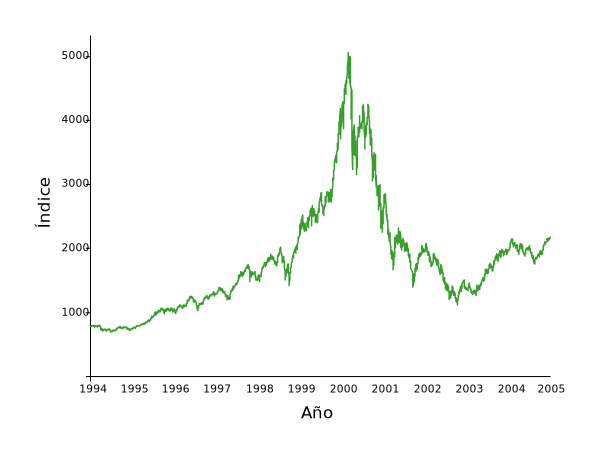
\includegraphics[width=150mm]{capitulos/graficos/comBubble} 
\label{fig:La burbuja de las punto com} 

	\footnotesize
	Fuente: Elaboración propia a partir de los datos recuperado en NASDAQ (2.012)

\end{figure}

Como se puede ver en la Figura \ref{fig:La burbuja de las punto com}, el índice NASDAQ se mantuvo triplicando su valor desde finales de 1.998 hasta marzo de 2.000. La especulación se incrementó enormemente. Comprar por Internet se convirtió en una actividad popular y había más de diez millones de comerciantes al día en Internet. También hubo escándalos fraudulentos como \emph{Enron}. A lo largo de 1.999 y también a principios del año 2.000, la Reserva Federal de Estados Unidos aumentó los tipos de interés seis veces, provocando que la economía perdiese velocidad. Por otro lado, muchas de las empresas que se basaban en Internet para obtener beneficios reportaron grandes pérdidas netas. Eran dos factores importantes para que los inversionistas reinterpretasen sus expectativas.

Cuando la burbuja explotó, más de 8 billones de dólares en valores de mercado, se evaporaron. Incluso las empresas líderes se derrumbaron, algunos ejemplos son: Amazon, Cisco Systems, Corning, JDS Uniphase, Nortel Networks, Priceline, Yahoo.com, entre otros. Todos ellos perdieron entre un 90 y un 99,7 por ciento del precio de las acciones.

\subsection{La burbuja inmobiliaria} 
Esta burbuja se conoce generalmente como la burbuja inmobiliaria, la burbuja de las hipotecas sub-prime o la burbuja de crédito, entre otros nombres. Sin embargo, se puede demostrar que no sólo afectó al sector inmobiliario, sino que también se materializó en otros sectores provocando una crisis global.

En este caso, vamos a centrar el estudio en la burbuja inmobiliaria española aunque no se ha de perder de vista la burbuja inmobiliaria en Estados Unidos.

En primer lugar, se puede plantear la siguiente cuestión, \emph{¿Qué es una burbuja inmobiliaria?} Según el blog de economía Gerencie.com: \emph{una burbuja inmobiliaria es un incremento excesivo e injustificado de los precios de los bienes inmuebles o bienes raíces, ocasionado generalmente por la especulación}.

\begin{figure}[!h] 
\caption{La burbuja inmobiliaria de España. Precio nominal medio de la vivienda nueva en España} 
\centering 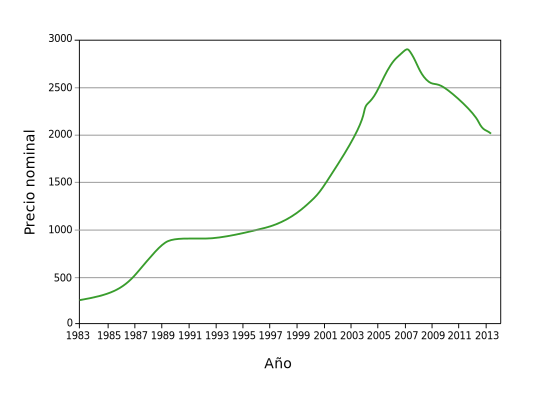
\includegraphics[width=150mm]{capitulos/graficos/precioVivienda} 
\label{fig:precioVivienda} 

	\footnotesize
	Fuente: Wikipedia Española

\end{figure}


\begin{figure}[!h] 
\caption{La burbuja inmobiliaria de Estados Unidos} 
\centering 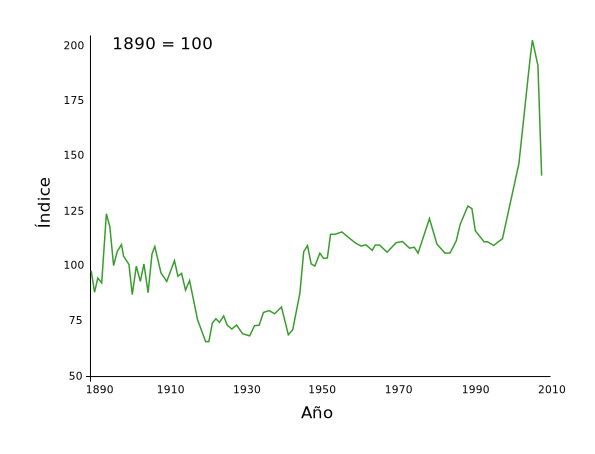
\includegraphics[width=150mm]{capitulos/graficos/HousingBubbleUSA} 
\label{fig:HousingBubbleUSA} 

	\footnotesize
	Fuente: Shiller Index

\end{figure}

Según el autor De la Dehesa (2.009), esta burbuja comenzó a gestarse al finalizar la Segunda Guerra Mundial incrementándose así, década tras década, el precio de la vivienda. Es de esperar que la población no de mayor importancia al hecho de que aumente el precio, ya que se ve como algo natural y se terminan olvidando los fundamentos económicos que refutan el comportamiento cíclico de ésta, es decir, que lo que en un momento dado sube, luego tiende a bajar y todo lo que aumenta abruptamente tiende a caer en exceso.

Una de las variables más condicionantes de la burbuja inmobiliaria es el tipo de interés. Un bajo tipo de interés proporciona una mayor demanda de créditos por parte de los clientes. Pero por otro lado, si los tipos de interés tienen una tasa alta, las entidades bancarias no hubieran concedido créditos a los clientes denominados \emph{NINJA}, probablemente hoy por hoy no se hablaría de crisis económica. En el mercado financiero se conoce a los clientes NINJA como a aquellos que no disponen de ingresos fijos, empleo fijo, o propiedades con las que saldar las deudas concertadas con las entidades bancarias. La palabra \emph{NINJA} es un acrónimo de \emph{No Income, No Job, no Assets}. \footnote{En castellano se traduce como no ingresos, no trabajo, no activos}. Al mismo tiempo, surgió el término \emph{titulización} que según la Real Academia de la lengua Española, titulizar se pude definir como: \emph{convertir determinados activos, generalmente préstamos, en valores negociables en el mercado}\footnote{Diccionario de la Real Academia de la lengua española}.

El antiguo método que empleaba la banca era el de \emph{comprar para mantener}. Este sistema se basaba en que los bancos obtenían su financiación a partir de los depósitos, prestando a su vez a largo plazo a clientes, para mantener las relaciones con éstos hasta el fin de los préstamos, es decir, varios años a posteriori. Las posibles inestabilidades se mitigan con la relación a largo plazo con los clientes, la existencia de sistemas de garantías de depósitos y la función de prestamista de última instancia de los bancos centrales.

Durante la primera década del año 2.000, el sistema da un giro de ciento ochenta grados hacia lo que se denomina \emph{originar para distribuir}. En este nuevo sistema, los bancos son meros intermediarios entre los clientes \footnote{Los potenciales generadores de riesgo de crédito.} y los financiadores \footnote{Los demandantes de dicho riesgo.}. El riesgo inicial existente intrínsecamente, se empaqueta y reestructura hasta conseguir el binomio rentabilidad y riesgo objetivo.

El nuevo sistema implantado, produjo un deterioro de las condiciones crediticias. El sector privado, desarrolló diferentes formas de titularizar hipotecas consiguiendo atraer una enorme cantidad de nuevo capital en la industria. Mientras tanto, el gobierno estaba permitiendo esta situación sin intervenir para garantizar mínimos lógicos de solvencia que respaldase esa operativa. 

El resultado de este cambio fue aportar grandes sumas adicionales de dinero disponible para la compra de viviendas y aumentar el tamaño del sector inmobiliario. Además, se animaba a los propietarios que ya tenían las primeras hipotecas, a que las aumenten o a que realizasen una segunda hipoteca sobre su inmueble para hacer nuevos consumos familiares. De este modo, aumentó fuertemente la cantidad de la deuda asumida por los consumidores. Se puede hacer una analogía afirmando que los consumidores utilizaban sus casas como un cajero automático.

A continuación se van a mostrar dos gráficos. El primero se corresponde con la burbuja inmobiliaria de España y el segundo con la burbuja inmobiliaria de Estados Unidos.

Como se puede comprobar en la Figura \ref{fig:precioVivienda}, en el momento en el que la burbuja estalló, los precios de las viviendas comenzaron a caer secuencialmente en picado. A mediados de 2.009, estos precios disminuyeron en más de un tercio de su máximo histórico. Muchos propietarios, se encontraron con que sus casas valían menos que la cantidad del dinero pactado en sus hipotecas y comenzaron a sucederse los impagos, deteniéndose la concesión de préstamos por parte de las entidades bancarias. Los mercados de crédito se congelaron y se convirtieron en instituciones incapaces de refinanciar su deuda a corto plazo.

Los valores con garantía hipotecaria, se vendieron a lo largo y ancho de todo el mundo, lo que provocó el debilitamiento de todos los sistemas bancarios mundiales. De este modo, se desencadenó una grave recesión mundial, con unas tasas de desempleo muy elevadas y en las que actualmente todavía hay sumergidos innumerables países, no tan sólo es el caso de España.

\section{Análisis descriptivo del concepto burbujas económicas} 
Como se anticipó en el epígrafe 1.2, es evidente que una burbuja puede manifestarse en diversos contextos y en diferentes clases de activos. También se ha podido apreciar que podría dar lugar a un efecto neto positivo como en el caso de la burbuja de la manía del ferrocarril, también a una redistribución de la riqueza como ocurrió en la manía de los tulipanes; o por el contrario sufrir un efecto neto negativo, como en la de Japón. Sin embargo, existen diferentes factores que vale la pena destacar.

\subsection{Factores que influyen en la formación de las burbujas económicas} 

Para comenzar, la primera variable fundamental es el \emph{precio}. Es la característica más notable de una burbuja ya que los precios aumentan enormemente en un corto período de tiempo, perdiendo la correlación con los valores fundamentales y alcanzando en muchas ocasiones precios desorbitadamente altos. Pero finalmente estos precios colapsarán y tendrán como resultado una caída muy abrupta. 

El segundo factor elemental es la \emph{inversión/especulación}. Como se ha podido comprobar a lo largo del capítulo, a cada burbuja van asociadas grandes cantidades de dinero que entran y salen del mercado.

La tercera característica se ha podido apreciar en el epígrafe anterior con la descripción de las burbujas económicas más importantes a lo largo de la historia. La mayoría de éstas, comparten un contexto común en su formación, como es el de una gran \emph{empresa emprendedora}, no tiene que ser como tal una empresa, puede darse como una idea innovadora para la población. Tras la creación de esta \emph{empresa} siempre hay una clara \emph{incertidumbre} sobre la rentabilidad de ésta, de su estrategia de negocios, de su capacidad en los mercados, etc. 

No es conveniente identificar a esta cuarta variable, que es el \emph{apalancamiento financiero}, como un factor en sí de la burbuja económica, pero aun así, se puede decir que el apalancamiento financiero es un término comúnmente conocido y que consiste en recurrir a la deuda para aumentar la rentabilidad de los accionistas \footnote{La rentabilidad financiera}. El posible aumento de la rentabilidad, tiene como contrapartida un aumento del riesgo financiero. Poniendo como ejemplo la burbuja de la Compañía de los Mares del Sur, ésta Compañía aceptó el pago inicial de los accionistas y el resto a pagar en cuotas. Por lo tanto, bien sea a través de pagos iniciales o por la abundancia de crédito, el apalancamiento se encuentra entre los agentes que participan en el proceso de formación de la burbuja.

Existe un quinto agente que es el \emph{gobierno}. En la mayoría de las burbujas económicas, y como se comprobará a lo largo del proyecto, sus respectivos gobiernos participan en diversas etapas de ésta tomando diferentes medidas. Por ejemplo, en el caso de los tulipanes, el gobierno trató de evitar el estallido de la burbuja. Por otro lado, en la burbuja de la Compañía del Mississippi, fue el propio gobierno quien fue gestando la burbuja económica en manos de John Law. 

En resumen, se podría argumentar que una burbuja, ocurre gracias a una perfecta mezcla entre variables importantes del mercado como son la incertidumbre, los tipos de interés, el apalancamiento y la intervención de los gobiernos. De este modo, los flujos de dinero masivos que se introducen en las burbujas provocan que los precios se disparen.

\subsection{Etapas de una burbuja económica}

Cada una de las burbujas económicas expuestas a lo largo del capítulo, ha quedado ilustrada por un gráfico. Independientemente de cuál de ellas se elija para apreciar la evolución de los precios, se puede valorar la similitud de la campana. Según el jefe del departamento de estudios globales, de la Universidad de Hofstra, El Dr. Jean-Paul Rodrigue, las principales etapas de una burbuja se pueden apreciar en la siguiente Figura \ref{fig:bubbleFases}:

\begin{figure}[!h] 
\caption{Fases de una burbuja económica} 
\centering 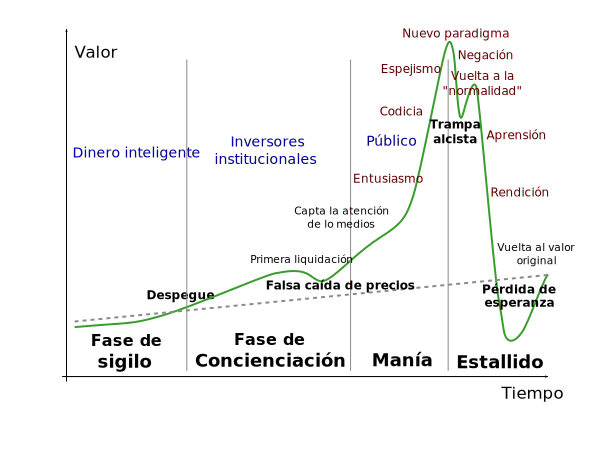
\includegraphics[width=150mm]{capitulos/graficos/bubbleFases} 
\label{fig:bubbleFases} 

	\footnotesize
	Fuente: Rodrigue (2.010)

\end{figure}


De una forma teórica, se pueden clasificar estas fases en:
\begin{enumerate}
	\item \emph{Sigilo}. Pocos inversionistas especializados se percatan de la revalorización sustancial y asumen el riesgo de ser pioneros. A este hecho, se le denomina \emph{dinero inteligente}, ya que introducen dinero en el mercado con cautela para que los demás participantes lo noten. Este tipo de inversionistas, pueden tener una información más fiable y más rápida, así como herramientas y conocimientos necesarios para afrontar los hechos en el mercado. Los precios de los activos se incrementarán gradualmente y sin la participación de los inversores masivos. El dinero inteligente, también ganará posiciones poco a poco.
	\item \emph{Concienciación}. La introducción de dinero realizada en la anterior etapa, es detectada por otros inversores que ponen más dinero sobre los activos y los empujan al alza. Nuevos inversores pueden adquirir los primeros beneficios provocando un aumento gradual del precio. Al final de esta etapa, los medios de comunicación se involucran y como resultado, el resto de inversores se introducen en el mercado. 
	\item \emph{Manía}. La tendencia de los precios es claramente al alza y los ciudadanos deciden invertir sus ahorros para poder percibir hipotéticos grandes beneficios en un futuro. Estás importantes cantidades de capital, generan expectativas aún mayores y alimentan los precios para que éstos aumenten. Sin embargo, el dinero inteligente invertido en la primera fase, junto con los inversores institucionales, se encuentra en \emph{silencio}, mientras que la venta de los activos está sobrevaluada para el resto de la ciudadanía inversora.

	Durante este periodo de \emph{locura}, todo el mundo trata de participar aunque no se tengan los conocimientos y la preparación adecuada para llevar a cabo transacciones inteligentes. Cuando el crédito es accesible y barato, esta fase dura mucho más tiempo de lo esperado. En este intervalo de tiempo, los medios de comunicación toman parte de la burbuja asegurando a los inversores que los precios han alcanzado una \emph{meseta permanente} con el fin de justificar los precios vertiginosos. La burbuja se comienza a volver más hostil y se encuentra a punto de eclosionar. 
	\item \emph{Estallido}. En un momento determinado y más o menos al mismo tiempo, todos los agentes implicados en el mercado se dan cuenta de que la situación ha cambiado. Aparece la desconfianza y el sentimiento de que las expectativas se desmoronan. Hay una etapa de negación, donde muchos inversores, embelesados por el mercado, tratan de convencer a todos de que el retroceso es sólo temporal. Este hecho provoca un pequeño resurgimiento, pero el espejismo tarda poco en desaparecer. Los descensos se desencadenan a cada cual más espectacular. El colapso se hace factible y los inversores en general se tienen que quedar con los activos sobrevalorados, mientras que el dinero inteligente, invertido en la primera fase, había dejado el mercado hace mucho tiempo. 
	
	Muchos agentes aprovechan la quiebra para adquirir este tipo de activos, ya que se produce una oleada de ventas a precios muy bajos. Sin embargo, la gente en ese momento, considera que estos activos están contaminados y es cuando vuelve a aparecer el dinero inteligente adquiriendo gangas a precios muy bajos.
\end{enumerate}

Es interesante destacar que los primeros en abordar el mercado, son los individuos con \emph{dinero inteligente}. Este tipo de inversionistas podrían tener algún tipo de monopolio en cuanto a información se refiere. Los segundos a tomar posiciones, son los inversores institucionales, lo que provoca la llamada de atención de los medios de comunicación quienes entran en juego a lo largo de la manía. 

\section{Diferentes teorías sobre las burbujas económicas}
En esta sección, se presentan las teorías sociales y psicológicas más relevantes que existen sobre las burbujas económicas.

Una de las teorías más sorprendentes, es la de la inexistencia de burbujas económicas defendida por Peter Garber (2.000). Para poder comprender la postura de este autor, hay que destacar la hipótesis de los mercados eficientes, a partir de ahora denominada: \emph{EHM} y que Peter Garber (1.990) la define como, \emph{la idea de que los precios que prevalecen en el mercado, hacen que sea imposible ganar unos beneficios económicos anormales provenientes de la propia negociación en ese mercado}. Esto quiere decir que en un mercado eficiente todos los bienes o títulos estarán perfectamente valorados, lo que evitará la aparición de sobre o infravaloración de los mismos. Esto tendrá como resultado que los inversores obtendrán un rendimiento sobre su inversión apropiada al nivel de riesgo asumido, ya que no es posible superar los resultados del mercado excepto a través de información privilegiada o de la suerte. Es por esta razón, por la que siempre hay inversionistas buscando información que les permita pronosticar con precisión los precios futuros del bien.


Garber defiende que los inversionistas basan sus decisiones en la percepción sobre los fundamentos del mercado. Si se da este caso, entonces el precio de la acción debe reflejar todos los factores fundamentales, y de acuerdo con la EHM y la definición de burbuja económica, se obtiene como resultado que las burbujas económicas en sí mismas no pueden existir. Por lo que este autor llega a la conclusión de que \emph{las burbujas están en divergencia con cualquier información económica razonable}.

Garber, también defiende que la especulación es meramente un factor psicológico pese a que se le puede dar un sentido económico y lo ilustra con las burbujas de la Compañía del Mississippi y de la Compañía de los Mares del Sur.  Ambos proyectos macroeconómicos llevados a cabo por los gobiernos de Francia y de Londres respectivamente, fracasaron porque tuvieron partes defectuosas dentro del plan ideado y porque los economistas de aquellos años, respaldados por estos gobiernos, no trabajaron día a día en las herramientas financieras que debían. Para los economistas no es de buen gusto aceptar que un \emph{experimento} ha fallado. 

En cuanto a los factores psicológicos se refiere, es importante señalar que proporcionan valiosa información y se consideran buenos indicadores a tener en cuenta en el tema a tratar. Esta teorías psicológicas serán desarrolladas a lo largo de este epígrafe, y tienen su base en el concepto psicológico keynesiano que desarrolló John Maynard Keynes (1.935), y al cual denominó \emph{espíritus animales,} 	\footnote{Texto ampliado en el Anexo 1} en su obra maestra \emph{La teoría general de la ocupación, los intereses y el dinero}, que fue publicado en 1.935. Por lo tanto, se han de dar unas pinceladas keynesianas como base.

Keynes habla de \emph{espíritus animales} como un término que describe los sentimientos que influyen en el ser humano y en su comportamiento, y que a su vez pueden ser mensurables en términos de \emph{confianza de los consumidores}	\footnote{Se trata de un indicador económico que mide el grado de optimismo que los consumidores perciben sobre el estado del mercado y sobre su propia situación financiera personal.} que ésta a su vez también puede ser medida por los \emph{espíritus animales}. Los inversores en general se suponen demasiado ignorantes para formar estimaciones fiables de los valores actuales. \emph{Su ignorancia conduce a la negociación a corto plazo y a la especulación}. Keynes concluye definiendo la expresión espíritus animales como \emph{el impulso espontáneo de la acción en lugar de la falta de acción} \footnote{Keynes, J. (1.935)}. Creía que, las acciones inducidas por este espíritu animal, eran producidas por la irracionalidad humana.
Con esta breve explicación de la teoría de Keynes se va a proceder a explicar cuatro teorías psicológicas.

\subsection{La teoría del más tonto}

Según esta teoría, defendida entre otros por Peter Garber (2.000), a los agentes del mercado que tienen un optimismo elevado en las acciones, se les denomina los tontos. Éstos se encargan de comprar activos sobrevaluados, con la intención de venderlos a un precio aún más alto a otros agentes del mercado - denominados los más tontos ya que tiene expectativas aún más altas que los anteriores o demasiado optimistas sobre los precios de los activos - y están dispuestos a especular con ellos porque creen que el precio no refleja el valor fundamental. El ciclo continúa con los tontos y los más tontos en el mercado hasta que la burbuja estalla cuando ya no hay más tontos dispuestos a comprar al precio máximo. 

\subsection{La teoría del comportamiento de manada} 

Este término proviene del concepto de pastoreo. Y no es más que un símil entre el comportamiento animal y el comportamiento humano. Esta teoría, apoyada por Peter Garber, afirma que las personas imitan las acciones, bien sean racionales o irracionales, de un grupo más grande de individuos. Es decir, la multitud de inversores compran y venden según se mueva el mercado.

Los análisis técnicos de mercado, se basan generalmente en este concepto, ya que su objetivo principal es detectar las tendencias del mercado, es decir, el comportamiento de manada para \emph{asegurar} inversiones. Este hecho no sólo se puede dar como figura individual, si no que también existen inversionistas institucionales como los fondos de inversión que también lo utilizan.

Para poder comprender dicha teoría de una forma sencilla y clara, se va a realizar una comparativa con un banco de peces. En un banco de peces, todos los miembros se decantan por seguir la dirección que toman los demás en su conjunto, sin una coordinación ni organización determinada. De este modo, en un mercado alcista, los inversores seguirán la tendencia especuladora hasta que ésta sea insostenible. En ese momento, el mercado procurará dar un giro de ciento ochenta grados para que los inversores comiencen a vender causando entonces, una caída brusca en el precio y dando lugar al final de la burbuja. Esta teoría del comportamiento gregario se da en otros aspectos de la vida humana como por ejemplo las modas. 

\subsection{La teoría de la extrapolación} 

El aspecto clave de la extrapolación de datos históricos, según los autores Fisher  \& Statman (2.002), se proyecta hacia el futuro con la base de que lo que ha ocurrido con ciertas condiciones, se va a repetir en un futuro que tenga el mismo contexto. En el caso de las burbujas se suele llevar a cabo una extrapolación de precios manteniendo la creencia de que  éstos continuarán su tendencia pasada en el futuro. El apoyo de este argumento proviene del hecho de que los inversores tienden a asociar los últimos rendimientos de determinados activos con retornos futuros, a la consecuencia de sobrepujar algunos activos de riesgo con el fin de mantener y alcanzar las mismas tasas del pasado. Sin embargo, este proceso conduce a un punto en que los beneficios ya no son positivos y los inversores no se sienten compensados  por el riesgo y se sucede el estallido de la burbuja.

\subsection{La teoría del riesgo moral}

Para poder explicar esta teoría se va a proceder a dar un ejemplo ilustrativo con el nivel de seguridad que puede haber en una casa. Este ejemplo ha sido recuperado de Wikipedia.

En una casa, los propietarios pueden decidir instalar una puerta acorazada, reduciendo así el riesgo de robo. Al mismo tiempo pueden ir reduciendo este tipo de riesgos hasta que las ganancias marginales de tomar precauciones sean iguales que los costes marginales de éstas, es decir, hasta que se obtenga mayor beneficio por cada precaución que se tome. Sin embargo, si los propietarios tienen concertado un seguro de hogar en el que se cubre el robo íntegro de la casa, tendrá menos incentivos instalar la puerta acorazada y aumentar así, la probabilidad de que se produzca un robo. 

Por lo tanto, en términos económicos, se podría definir el riesgo moral como, cada movimiento que altera la relación rentabilidad y riesgo. Si se da el hecho de que el agente que asume el riesgo sufre una situación fatal, entonces éste consigue un incentivo para adquirir un nivel de riesgo por encima de sus posibilidades. De este modo puede generar la inestabilidad del sistema y la burbuja económica podría surgir como una consecuencia.



\section{¿Puede ser positiva la existencia de una burbuja económica en la sociedad?} 
En este epígrafe, se discutirá si las burbujas tienen efectos positivos o efectos negativos sobre el bienestar económico general y se explicarán las posibles consecuencias. 

Como se ha mencionado anteriormente, no todas las burbujas son negativas ya que se necesitan ciertos tipos específicos de éstas en nuestro sistema monetario. Por ejemplo, algunas pueden conducir a una expansión de los sectores económicos que sin su existencia nunca hubiesen tenido lugar. 

Se va a estudiar en qué momento es más conveniente o inconveniente actuar, es decir, en el inicio, durante o en su defecto, y si se diese el caso, antes de la burbuja porque existan signos claros de ésta, o por el contrario después del estallido.

\subsection{Burbujas económicas positivas}

En primer lugar, convendría dar explicación acerca de lo que es el \emph{dinero fiduciario}, para ello se puede decir que el dinero fiduciario tiene su fundamento en la confianza de la ciudadanía sobre esa moneda y en las entidades encargadas de emitirla, ya que ésta no tiene respaldo material.

A la hora de catalogar al dinero fiduciario como una de las mayores burbujas económicas en si mismas, se tiene que tener en cuenta que su valor fundamental es cero. En el año 1.971, el entonces presidente de los Estados Unidos Richard Nixon, eliminó la convertibilidad del patrón oro, lo que supuso la pérdida de relación entre el dinero papel y el tan codiciado metal. Entonces se puede plantear una pregunta, \emph{¿Qué podría asignar valor al dinero de una forma completamente arbitraria?} La respuesta es: la confianza y comodidad. 

Según Samuelson (1.958), \emph{la confianza} que confiere el dinero, permite intercambiar a los agentes, bienes y servicios con la garantía y respaldo del Banco Central. Y por otro lado, \emph{la comodidad} que aporta el dinero fiduciario, ya que éste sirve como un medio de intercambio. Y por último, destacar que este tipo de dinero se utiliza para pagar  impuestos, lo que le otorga un valor añadido.

De todas las burbujas expuestas a lo largo del capítulo, los dos mejores ejemplos que representan el espíritu positivo de una burbuja económica, en cuanto a la expansión de los sectores económicos se refiere, es sin duda la manía del ferrocarril. Un total de 10.000 kilómetros fueron construidos como resultado de los proyectos autorizados entre 1.844 y 1.846. Y en segundo lugar, la burbuja punto com, ya que amplió los sectores de telecomunicaciones e introdujo a la población en la nueva era de Internet. 

\subsection{Burbujas económicas negativas}

Tirole (1.985), es uno de los primeros autores que afirmó que las burbujas económicas tenían efectos divergentes en diferentes modelos económicos. También defiende que, al comienzo de la burbuja económica, los compradores y vendedores se introducen en el mercado con un conjunto de informaciones comunes y por lo tanto el conocimiento general es homogéneo, reina la racionalidad y los recursos son asignados eficientemente antes de las negociaciones. También argumenta que tan sólo unos pocos agentes pueden realizar compras y ventas de forma infinita.

Hay que destacar que al autor Peter Diamond (1.965), defiende que uno de los motivos de la existencia de las burbujas puede ser la infinidad de hogares que pueden negociar con activos financieros. Pese a esta teoría, defiende que una burbuja, sólo se le podrá denominar como tal, cuando crezca al mismo tiempo y de la misma forma que el resto del mercado. 

Como conclusión, se puede decir que para poder considerar que una burbuja económica es una burbuja en sí misma, el mercado ha de crecer de menara diferente a los ratios que se consideran apropiados, y a su vez, poseer una enorme acumulación de capital. Para poder comprender el crecimiento paralelo con el mercado, cabe destacar la definición de \emph{burbuja asintótica}: \emph{Se trata de una burbuja que crece al mismo tiempo que lo hace el resto de la economía, teniendo en cuenta que el consumo es eficiente}.	\footnote{Diamond, (1.965)}

A posteriori, los autores Saint-Paul (1.992), Grossman Yanagawa (1.992)y King And Ferguson (1.993), modifican la teoría de Diamond defendiendo que las burbujas pueden darse sin la existencia de una entrada de capital excesiva, argumentando así, que estos niveles de capital dependen de la productividad. Concretamente los autores Grossman y Yanagawa (1.992) ampliaron algunos modelos de Tirole para incluir a las economías que crecían en el largo plazo y a una tasa endógena. La conclusión a la que llegaron en su tesis fue que \emph{las burbujas retardan el crecimiento de la economía, posiblemente incluso en el largo plazo y reducen el bienestar de todas las generaciones nacidas tras la burbuja económica}. Concluyen también, afirmando que el impacto de la explosión de la burbuja, podría ser beneficioso para la generación actual pero puede tener graves consecuencias futuras ya que retarda el crecimiento económico para éstas.

Los mejores ejemplos de este tipo de burbujas económicas son las inmobiliarias, ya que es la clase de burbuja más cercana en el tiempo y además, un gran número de importantes economías mundiales occidentales están inmersas en ella. 

Una vez realizado este análisis en profundidad de qué es una burbuja económica en todos sus sentidos, se va a proceder a explicar tres de las burbujas más relevantes de la historia. En el capítulo dos se desarrollará a la tulipomanía, en el capítulo tres se introducirán la burbuja de la Compañía del Mississippi y el sistema de John Law y para finalizar se explicará la burbuja de la Compañía de los Mares del Sur, sustancialmente ligada a la desarrollada en el capítulo tres. 



\chapter{Tulipomanía}

\section{Contexto histórico}

La tulipomanía es probablemente la primera burbuja económica de la historia de la que existe información detallada y que ha sido estudiada en profundidad por economistas e historiadores. Tuvo lugar en Holanda, en el período que abarca del año 1.630 al 1.637.

Se ha de situar a Holanda en un contexto de auge económico y de desarrollo. Pocos años atrás, Holanda se había declarado independiente del Imperio español. De este modo, para instaurar su propia autonomía comercial internacional, tuvo que desarrollar su propia flota naval, aprender a tripularla y desplegarla. A la cabeza de esta iniciativa se encontraba la Compañía de las Indias Orientales, empresa cuya propiedad se dividía entre el gobierno y el sector privado. Esta empresa navegaba alrededor del mundo y se encargaba de obtener productos poco comunes en Europa para venderlos y obtener amplios beneficios. Con las provincias holandesas convertidas en el principal centro de comercio del norte de Europa, se alcanzó la llamada edad de oro holandesa.

El marco cronológico de la tulipomanía, es la Europa del siglo XVII. Al igual que en la actualidad, las clases sociales altas atribuían gran valor a aquellos objetos indicadores del elevado estatus social al que pertenecían. En el siglo XVII, estos objetos eran mansiones, jardines, e incluso ciertas flores exóticas, como el tulipán.

\section{El tulipán}

La primera referencia que existe sobre el tulipán, data de hace más de mil años y se establece su procedencia en Anatolia, región que se corresponde a la actual Turquía. 

\emph{Lale} es la traducción al turco y contiene las mismas letras que el Dios islámico \emph{Alá}, por lo que era considerada una flor sagrada. El tulipán, debido a su sencillez y belleza, encandiló a los altos representantes del Imperio Otomano.

Es conveniente, explicar previamente determinados aspectos relacionados con el desarrollo biológico del tulipán para la compresión del comportamiento del mercado de tulipanes que se llevó a cabo en Holanda.

En particular, se describirán brevemente los tiempos de desarrollo de un bulbo de tulipán, el florecimiento de dicho bulbo, la aparición de vástagos y la asombrosa aparición de tulipanes policromáticos, comúnmente denominados en inglés \emph{tulip flames}. 

\begin{figure}[!h] 
\caption{Semper Augusta} 
\centering 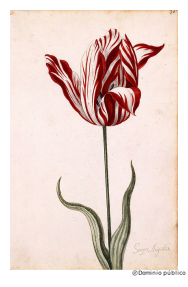
\includegraphics[width=50mm]{capitulos/img/semperAugustus} 
\label{fig:semperAugustus} 
\end{figure}

Los tulipanes son cultivados a partir de semillas. Éstas podrían tardar de tres a cinco años en convertirse en bulbo y de cinco a diez años en producir una flor. Cada bulbo, tiene el aspecto de una pequeña cebolla y puede llegar a producir al año uno o dos vástagos además de varias semillas. Un vástago es un pequeño bulbo que surge en la tierra a partir del bulbo matriz.

Tradicionalmente, la compra-venta de bulbos de tulipán se producía a lo largo de los meses de verano, cuando la flor nacida del bulbo, ya había florecido por el mes de mayo o junio (dependiendo de la clase de tulipán que se tratase). A continuación, la flor era cortada y vendida, y el bulbo se desenterraba, se envolvía en papel y se mantenía en lugares secos para su posterior inspección y replantación en el mes de septiembre.

Los tulipanes más codiciados por la sociedad en el siglo XVII, fueron los que tenían un único color como el rojo y el púrpura. Además, en 1.620 comenzaron a surgir tulipanes con extrañas y llamativas estructuras cromáticas o comúnmente denominados \emph{tulipanes con llamas}. Estas llamas, recorren simétricamente el centro de los pétalos y los bordes tal y como se puede apreciar en la Figura \ref{fig:semperAugustus}. Esta viva coloración que fascinó a los holandeses, fue causada por un virus que infecta los bulbos. Este hecho, fue un misterio en su momento ya que no se le dio explicación hasta el año 1.928, gracias a los trabajos de la doctora Dorothy Cayley. Este proceso impredecible añadió encanto y valor a los tulipanes como se comprobará a lo largo del capítulo.

\section{Origen y evolución del mercado de los tulipanes en Holanda}

La aparición del tulipán en Holanda fue posible gracias a dos personas fundamentalmente, Busbeq y Clusius.

En primer lugar, Ogier Ghiselin de Busbecq que fue un diplomático, escritor y herborista flamenco del siglo XVII, más conocido como \emph{Busbeq}.

Fue nombrado por Fernando I de Habsburgo como embajador del Sacro Imperio Romano Germánico en la corte de Solimán I el Magnífico. Fue enviado a Constantinopla a finales de 1.554 donde permaneció hasta 1.562. Durante esos años escribió las \emph{Cartas Turcas}, en las que relata sus experiencias y viajes en tierras del Imperio Otomano. En esta obra, a menudo resaltaba la hermosura de los jardines otomanos, con sus misteriosas flores rojas de tulipán. A su regreso a Austria, decidió llevar consigo algunos bulbos de esta planta. 

Busbeq entabló amistad con \emph{Carolus Clusius}, segundo hombre importante en la historia de la aparición del tulipán en Holanda. Se trató de un humanista, médico y botánico holandés, quien en 1.573 fue invitado por el emperador Maximiliano II de Habsburgo para trabajar para el jardín botánico de Viena. En ese lugar, Clusius plantó los bulbos de tulipán que con anterioridad Busbeq le confirió. Cuatro años más tarde, Clusius fue despedido y a lo largo de veinte años, se dedicó a viajar por toda Europa en busca de nuevos ejemplares.

En el otoño de 1.593, fue nombrado profesor honorario de botánica en la Universidad de Leiden, donde supervisó la creación de un jardín botánico. Entre la multitud de plantas del jardín, se encontraba su propia colección de bulbos de tulipán. En la primavera siguiente, es decir, en 1.594, surgieron los primeros tulipanes florecidos en el norte de Holanda. Una noche en la que Clusius se encontraba de viaje en Inglaterra, desenterraron su colección y la robaron.

Estos ladrones, de los que se desconoce su identidad, convirtieron a estos bulbos en los progenitores de las flores que más tarde inundarían los Países Bajos. A partir de este momento, comenzó el comercio del tulipán.

La ciudad holandesa de Haarlem, fue una de las primeras en llevar a cabo transacciones con tulipanes. El rápido enriquecimiento de una parte de la población hizo que otras ciudades, como Rotterdam o Leiden, tomasen ejemplo de ello, extendiéndose así el mercado de norte a sur y de este a oeste del país. Esta extensión del cultivo del tulipán y su comercio asociado, fue uno de los desencadenantes de la Edad de Oro holandesa.

Hasta principios de los años 30 del siglo XVII, el mercado de los tulipanes estaba compuesto por hombres sensatos de negocios, comerciantes ricos, cuyas fortunas no se verían afectadas por un fallido negocio de compra-venta de bulbos. También los herboristas, que poseían un amplio conocimiento de tan codiciada flor, eran partícipes en las transacciones. Pero el mercado alcanzó tal fama que las clases sociales medias y bajas también se introdujeron en él, realizando inversiones modestas y provocando un boom de inversiones. La mayoría de estos inversores de clase social media utilizaban los bulbos para la especulación. A pesar del gran número de variedades de tulipán, la oferta seguía siendo muy limitada y la demanda muy elevada.

\subsection{Tipos de contratos}

Para poder comprender el funcionamiento del mercado de tulipanes a partir de 1.634, se han de explicar los diferentes tipos de contratos que se dieron.

En primer lugar, los contratos de futuros. Garber (2.000) argumenta que, el comercio llevado a cabo en las tabernas, era un mercado plenamente de futuros: \emph{En la fecha de liquidación del contrato, se espera sólo el pago de la diferencia entre el contrato y el precio de liquidación. Este mercado no fue tan diferente a los mercados de futuros que operan actualmente}.

En segundo lugar, los contratos a plazos. Según informaciones que se han podido recopilar de contratos notariales y contratos menos formales de compra-venta de la época, parece ser que al menos algunas operaciones consistieron en una complicada cadena de contratos bilaterales a plazo que unen a varios vendedores y compradores. No existía ningún mecanismo de compensación central, pero en ocasiones los nuevos compradores acordaron asumir la deuda presente del vendedor, es decir, \emph{cuando mi comprador me pague, yo te lo pagaré}.

Y por último, los contratos al contado. Cabe destacar en este tipo de contratos, que los bulbos de tulipán no necesitan ser plantados en el campo con unas condiciones determinadas, sino que los tulipanes también crecen en macetas. Los individuos participantes en el mercado, regularmente tenían medios financieros para obtener vasijas hechas especialmente para el cultivo de la planta. De este modo, los tulipanes en macetas estarían disponibles para la venta y entrega inmediata. En segundo lugar, el desenterramiento de los tulipanes o en su defecto el transporte de estos, es posible pero no se recomienda, porque siempre existe un riesgo de dañar la planta. La opción de contratos con entrega inmediata, incluso en el período comprendido entre los meses de septiembre y de mayo-junio, es factible hasta el día 5 de febrero 1.637, última subasta de tulipanes con precios elevados.

\subsection{Las tabernas}

A continuación se explicará el mercado de tulipanes en las tabernas holandesas. En estos lugares se gestaba el comercio con un mayor grado de especulación. A los grupos sociales, tanto de taberneros como de clientes, se les denominó \emph{colleges}.

Haciendo una analogía para comprender el concepto de \emph{colleges}, se puede asemejar a las hermandades. Estas \emph{hermandades} estaban formadas por un núcleo de comerciantes regulares que se reunían dos o tres veces por semana y por lo general a la caída del día. Para pertenecer a este grupo, el individuo interesado debía de afiliarse a la compañía de los floristas, que poseían su sede en las diferentes tabernas de las ciudades. Así, cada miembro poseía una placa, a modo de código, con la que podía mercadear con los tulipanes a su antojo. Estas hermandades suponían un sistema muy intenso de redes sociales ya que aunque había que pertenecer a los colleges. Aún así, la accesibilidad era muy rápida y sencilla.

Este mercado se volvió mucho más arriesgado en el momento en el que se fueron incorporando individuos que no tenían ningún tipo de conocimiento acerca del funcionamiento del mercado. De este modo, el mercado se fue transformando poco a poco en una suerte de juego de azar en donde se podía doblar la cantidad jugada, y pagar así la deuda por el bulbo, o por el contrario, perder el bulbo y adquirir una mayor deuda alcanzando la completa ruina.

La mayor parte de la información recopilada acerca de las transacciones entre 1.636 y 1.637 de la que se dispone en la actualidad, es de una serie de contratos de tulipán individuales. Por lo general, estos documentos formaban parte del arbitraje a través de los notarios y de los tribunales. No se ha podido obtener información sobre la importancia relativa de las sesiones de negociación en las tabernas ya que no se dieron detalles sobre el tipo de transacciones, precios o volúmenes de comercio. Este tipo de negocio, era conocido en Holanda como \emph{Wind handle}, es decir, el negocio del aire.

Surgieron dos métodos de compra-venta de bulbos:

El primero, consistió en que tanto el comprador como el vendedor escribían un precio en un libro y elegían a una serie de mediadores que eran los encargados de fijar un precio intermedio, y mediante el arte del regateo conseguían cerrar el acuerdo. Este procedimiento se ejercía bien con contratos inmediatos o con contratos futuros.

El segundo método era la subasta. Se daba un precio de salida para una determinada transacción de bulbo, bulbos, tulipán o tulipanes, y se va incrementando este precio de salida hasta que ningún individuo está dispuesto a superar la oferta final.

En ambos casos, la gran mayoría de los negocios entre compradores y vendedores se llevaban a cabo con la presencia de los mediadores entendidos del mercado y que poseían amplios conocimientos acerca de los tulipanes.

Todos los contratos llevaban un suplemento de comida, bebida y tabaco llamado  \emph{Wijnkoop}, cuya traducción al castellano es  \emph{compra de vino}. Este coste era soportado por el comprador final y aproximadamente se correspondía con el 2,5 por ciento de la cantidad final pactada. Por otro lado, en el caso de la venta de futuros, si el bulbo desenterrado no se correspondía con las características pactadas meses antes, la venta quedaba anulada. En el caso de que se hubiese acordado un sistema de garantías, el avalista del comprador, bien sea amigo o pariente, garantizaría la devolución del pago y por lo tanto el vendedor podía atenerse a él.

A lo largo de la temporada de siembra del año 1.635, momento en el que los precios comenzaron a incrementarse, se produjo un cambio fundamental en la forma de comercialización de los bulbos en Holanda. Cada vez más a menudo, se vendían bulbos a peso mientras que éstos todavía se encontraban plantados en el campo. Tan sólo un \emph{pagaré}, indicaba los detalles del bulbo, incluyendo su peso en la siembra y el momento en el que se iba a proceder a desenterrarlo.

El peso de los bulbos se comenzó a medir en Azen o ass, una unidad de medida extremadamente pequeña que equivalía aproximadamente a una vigésima parte de un gramo, es decir, 0,05 gramos. Pagar en peso, era una manera más justa para evaluar el precio, ya que un bulbo inmaduro costaba menos que uno más maduro. La utilización de esta unidad de medida provocó el aumento del precio de los bulbos más pesados. Un bulbo que se planta en septiembre u octubre es probablemente mucho más pesado que en el momento en el que se desentierra, debido a que ha sufrido una floración. Lo que alentaba a la especulación en los siguientes meses estivales. Se puede afirmar, que el precio de los bulbos podría haber aumentado de un tres a un cinco por ciento en el transcurso de estos nueve meses, dependiendo del peso.

Esta nueva unidad de medida fue muy expandida y se comenzaron a vender grandes cantidades de bulbos a peso, es decir, surgió una nueva modalidad de transacciones, los contratos a granel. Lo que provocó que los precios aumentasen de nuevo poco a poco pero muy constantemente. Estos contratos al peso, tienen el mismo funcionamiento que los contratos de bulbos pero de una forma mucho más masificada, ya que se compran y venden grandes sumas de bulbos por cantidades enormes de florines.

\subsection{Estallido de la burbuja}

Con el desarrollo de los diferentes contratos explicados anteriormente y su progreso en las tabernas, además de la creación de la nueva unidad de medida, con la que surgieron los contratos a granel, el mercado fue adquiriendo consistencia y fue evolucionando de una forma mucho más rápida de lo que lo hacía cualquier otro mercado y por lo tanto aumentaba el propio poder adquisitivo de la población.

La burbuja especulativa no tardó en estallar. Los precios se incrementaron más rápidamente a partir de octubre de 1.636 y los contratos a granel fueron los más utilizados en diciembre de ese mismo año, otorgando al mercado un impulso final. A finales del 36, personas ajenas al mercado, predijeron una caída de precios inminente y en enero de 1.637 los precios aumentaron más rápido y los comerciantes sospechaban que la situación comenzaba a ser insostenible. Por otra parte, las redes sociales densas por parte de los colleges en las tabernas, provocaron que este conocimiento fuese común para todos los comerciantes.

El tres de febrero de 1.637, en la ciudad de Haarlem, se produjo el primer descenso de precios de una forma totalmente inesperada. El cinco de febrero del mismo año, en la ciudad de Alkmaar, el precio del tulipán consiguió su máximo histórico con la subasta, por parte de un orfanato que tutelaba a los siete hijos de un coleccionista fallecido. Éste poseía una serie de tulipanes de una rareza extrema. La subasta se llevó a cabo para salvaguardar la manutención de los sucesores y muchos holandeses se agolparon a las puertas del orfanato para poder participar en la mencionada subasta. Los 99 bulbos de tulipán fueron vendidos por 90.000 florines, es decir, era un contrato a granel ya que si se equipara tal cantidad de florines a los actuales euros, equivaldría aproximadamente a 7,6 millones de euros. El siete de febrero, el negocio se derrumbaba en los principales puntos de comercio holandeses.

De este modo, se puede asegurar que la burbuja estalló el ocho de febrero de 1.637, ya que ante nuevas subastas de tulipanes, no hubo compradores.


\subsection{Sátiras y fuentes de recopilación de datos sobre los precios de los tulipanes}

Con todo lo acontecido en la tulipomanía, no tardaron en aparecer numerosos folletos y obras de arte satíricas, donde se ridiculiza la exuberancia irracional de muchos participantes en el mercado de los tulipanes, como se puede apreciar en la Figura \ref{fig:Satire Of Tulip Mania} .


\begin{figure}[!h] 
	\caption{Fragmento de \emph{Satire Of Tulip Mania}, por Brueghel} 
	\centering
	\includegraphics[width=80mm]{capitulos/img/fragmentoSatireOfTulipMania-Brueghel} 
	\label{fig:Satire Of Tulip Mania} 
\end{figure}

Se pueden destacar los folletos publicados por Adriaen Roman en la ciudad holandesa de Haarlem. En estos folletos se mantiene un diálogo entre dos personajes principales, \emph{Gaergoedt}, y \emph{Waermondt}.

Gaergoedt interpreta un papel de comerciante activo y responsable de bulbos, que se compromete a educar a Waermondt en el mercado del tulipán con el fin de explicar y defender las acciones emprendidas por los consumidores. Por otro lado, Waermondt, relata cuentos moralistas con los que se pretende resaltar la insensatez en diversos aspectos de la tulipomanía. Una de las características más valiosas de estos diálogos es que se reproducen contratos reales de ventas de bulbos y da referencias aproximadas de los precios alcanzados por los bulbos de principio a fin del fenómeno.

No existe una sola fuente completamente fiable en cuanto a precios de los tulipanes se refiere. Existen alrededor de cuatrocientos precios diferentes y la gran mayoría de ellos hacen referencia a los máximos alcanzados por las diferentes clases de tulipanes.

Para superar esta ausencia de información, algunos autores han adoptado diferentes estrategias, como por ejemplo, confiar en los folletos publicados y escritos entre febrero y mayo de 1.637 por Adriaen Roman.

Por ejemplo, en el primer diálogo entre Gaergoedt y Waermondt, se afirma que \emph{algunos precios de bulbos despuntaron hasta tal punto que alcanzaron cifras desorbitadas}. Hay que recordar que estos diálogos están destinados a ilustrar el carácter dramático de este escandaloso aumento de precios.

Un enfoque más prometedor, es el que realiza Garber (2.000), quien genera dieciséis gráficos que muestran la evolución de los precios de las diferentes variedades de tulipanes. Estos gráficos demuestran que los precios aumentaron considerablemente, aunque no se pueden obtener conclusiones certeras acerca de la trayectoria de los precios. El método empleado, establece un patrón con una línea recta entre diferentes precios. Los precios utilizados pertenecen a diferentes fuentes de información, por lo que en ocasiones se emplea una media y en otras ocasiones accede a fiarse de un dato terminado.

Como se podrá comprobar a continuación, se puede apreciar un aumento gradual en la primera fase de la tulipomanía y más tarde, se da una pendiente mucho más empinada próxima al final de la burbuja. Como también existe escasez de datos tras el estallido de la burbuja, Garber se ve obligado a depender de los precios de venta entre 1.642 y 1.643 realizando de este modo una media anual. Sin embargo, Garber concluye que, \emph{la crisis en febrero de 1.637, en cuanto a los tulipanes se refiere, no fue de extraordinaria magnitud} y la asume simplemente como una caída de precios gradual para el período comprendido entre 1.637 y 1.642. Garber considera que esta caída entra dentro de la normalidad del funcionamiento del mercado, es decir, Garber razona que la tulipomanía no es una burbuja económica como tal.

En las páginas posteriores se reflejan los gráficos de precios de algunos de los tulipanes más destacados a lo largo del desarrollo de la tulipomanía según las estimaciones de Peter Garber. Se corresponden a las figuras \ref{fig:Semper Augusta}, \ref{fig:Admirante Van Der Eyck}, \ref{fig:Admirante Liefkens} y \ref{fig:Switsers}


\begin{figure}[!h] 
\caption{Semper Augusta} 
\centering \includegraphics[width=150mm]{capitulos/graficos/SemperAugusta} 
\label{fig:Semper Augusta} 
	\footnotesize
	Fuente: Estimaciones de Peter Garber (2.000)
\end{figure}

\begin{figure}[!h] 
\caption{Admirante Van der Eyck} 
\centering \includegraphics[width=150mm]{capitulos/graficos/AdmiranteVanDerEyck} 
\label{fig:Admirante Van Der Eyck} 
	\footnotesize
	Fuente: Estimaciones de Peter Garber (2.000)
\end{figure}

\begin{figure}[!h] 
\caption{Admirante Liefkens} 
\centering 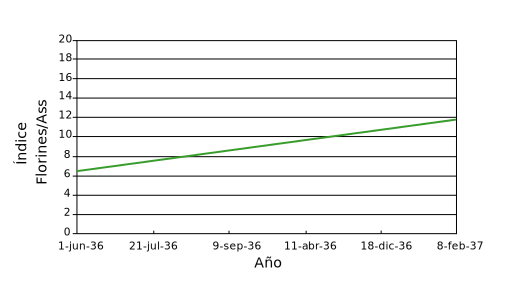
\includegraphics[width=150mm]{capitulos/graficos/AdmiranteLiefkens} 
\label{fig:Admirante Liefkens} 
	\footnotesize
	Fuente: Estimaciones de Peter Garber (2.000)
\end{figure}

\begin{figure}[!h] 
\caption{Switsers} 
\centering \includegraphics[width=150mm]{capitulos/graficos/Switsers} 
\label{fig:Switsers} 
	\footnotesize
	Fuente: Estimaciones de Peter Garber (2.000)
\end{figure}


En cuanto al momento del colapso, el primer lugar donde se produjo un descenso de precios fue en la ciudad de Haarlem el 3 de febrero. En los escritos de Adrien Roman, el protagonista Waermondt, narra el episodio donde los miembros de una hermandad decidieron poner a prueba la confianza del mercado, poniendo a la venta gran cantidad de tulipanes comunes como lo eran \emph{Switsers o Croonen} donde sólo se dio un comprador y éste mismo comprador ofreció diferentes precios en las tres subastas donde los tres vendedores aceptaron su oferta, a pesar de que la suma que ofreció fue una sucesión a la baja, comenzando en un 15 por ciento por debajo del precio de ese momento, continuando en un 25 por ciento y finalmente llegando al 35 por ciento. La noticia de esta caída en picado de los precios se extendió por todo el pueblo, pero no por el resto de Holanda. Dos días más tarde, en una subasta en Alkmaar, se alcanzaron los precios máximos.

Las notas de Gaergoedt ratifican la dificultad de establecer un nivel de precios tras el estallido de la burbuja y lo expresa en esta frase: \emph{Desde que no existe demanda, todo el mundo permanece en silencio}. Estima que tras el estallido, un jardín con tulipanes comunes no tenía ni la centésima parte del valor de hace tan solo unas semanas. Esto se puede comprobar con un claro ejemplo, un bulbo que valió en noviembre de 1.636 cuatrocientos florines, tras el estallido de la burbuja su precio descendió a veintidós florines, lo que supondría desmentir la tesis de Garber de caída de precios constante. 

Las fuentes de información son un aspecto clave para la realización de un exhaustivo estudio de precios. El fallecido profesor de la Universidad de Stanford, Earl. A. Thompson (2006), en su estudio \emph{The Tulipmania: Fact or Artifact}, ratificó que el aumento de los precios de los tulipanes a principios de 1.637 se debió a una serie de cambios en los instrumentos del mercado de los contratos futuros. Este autor, basa sus estudios en la validez de un índice generado por él mismo a través de precios relativos constantes, y que permite comparar diferentes tipos de tulipanes. Como punto negativo, se ha de señalar que no tiene en cuenta dos aspectos fundamentales como son, el espacio temporal, ya que no emplea el mismo momento temporal para todos ellos; y que evalúa al mismo tiempo los diferentes contratos\footnote{Los contratos con los vástagos de los bulbos, con los propios bulbos y con los bulbos vendidos a granel.} sin tener en cuenta que el valor de las transacciones no es igual para cada uno de ellos. A continuación se muestra la Figura \ref{fig:Precios de la tulipomanía según Thompson} donde se puede observar gráficamente su estudio:

\begin{figure}[!h] 
\caption{Precios de la tulipomanía según Thompson} 
\centering 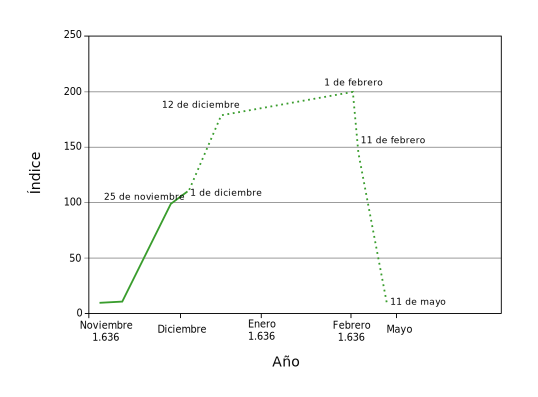
\includegraphics[width=150mm]{capitulos/graficos/Thompson} 
\label{fig:Precios de la tulipomanía según Thompson} 
	\footnotesize
	Fuente:  Earl A. Thompson (2.007)
\end{figure}

Thompson concluye que la centenaria literatura ha tergiversado la verdadera historia de la Tulipomanía. Pero por el contrario, da credibilidad a una serie de precios de los tulipanes de antes, durante y después de Tulipomanía, ya que afirma que proporcionan una información notable de los precios de mercado eficiente. Defiende que en su gráfico, los precios se pueden observar con rapidez y precisión, y se refleja la economía subyacente de un mercado en el que la euforia se traduce en ganancias y la decepción en pérdidas de capital.

En resumen, los datos de Garber y de Thompson no son de todo fiables. Las fluctuaciones de precios no son apoyadas por los fundamentos del mercado, ya que por ejemplo Garber ignora los puntos clave descritos en el párrafo anterior. Realizar afirmaciones más precisas sobre el precio, como por ejemplo cuándo y cómo se produjeron ciertos hechos en la burbuja económica es muy complicado. Por otro lado, Thompson ignora los problemas de la agregación de información de precios en los diferentes momentos temporales, aplicados a las diferentes formas de compra-venta de bulbos. Pese a que los datos son limitados, indican un rápido aumento entre diciembre de 1.636 y enero 1.637, seguido de un descenso brutal.

Para finalizar este epígrafe, hay que desatacar que por ejemplo Garber, establece una aproximación más bien gráfica, ya que realizar afirmaciones más precisas sobre cuándo y cómo se produjeron ciertos hechos en esta burbuja es muy complicado. En cuanto a Thompson, éste ignora los problemas de escasez de datos anteriormente descritos. Como conclusión al estudio de precios, se puede afirmar que los datos de Garber y de Thompson no son cien por cien fiables debido a la escasez de información que la tulipomanía sufre. 


\subsection{Influencia de la redes sociales} 

Para alcanzar una mayor comprensión de cómo se fueron desencadenando los hechos en la tulipomanía, se debe tener en cuenta un factor moderno como son las redes sociales, pero que inconscientemente ya era patente en el siglo XVII.

En primer lugar, se debería destacar la audacia de los vendedores, cada vez más experimentados, que se percataron de que cuanta más gente conociese su producto, más aumentarían las ventas y los precios de éstos, por lo que se creó el primer catálogo floral de ventas titulado \emph{El catálogo floral}, cuyo autor fue Emanuel Sweertl, también comerciante de tulipanes. Dicho libro, con pobres ilustraciones de los tulipanes en venta, hizo que se exportase en mayor medida tan codiciada flor. A raíz de este descubrimiento publicitario, se escribieron otros muchos que consiguieron ser número uno de ventas y provocaron, como bien había predicho Sweertl, el incremento del precio de los tulipanes.

Pese a la existencia de los catálogos florales, se puede percibir la ausencia de uno de los elementos más importantes y que hoy en día es imprescindible, los medios de comunicación. La importancia de éstos proviene de ser una de las necesidades primarias del ser humano: \emph{la interacción social}. Además, en la actualidad influye la \emph{opinión pública}. Como ejemplo, la influencia que tuvieron los medios de comunicación al mando de   Hitler como táctica para manipular a la sociedad alemana para que apoyara su ideología. Retomando la tulipomanía, es destacable la ausencia de periódicos regulares para cubrir la evolución del mercado de los tulipanes, el colapso de los precios y la consecuente crisis. Los periódicos, surgieron en las ciudades más desarrolladas de Holanda en el año 1.660, tres décadas después de la tulipomanía.

Otro de los aspectos a tener en cuenta, en el desarrollo de esta burbuja, es la eficacia de las redes sociales y las intensas normas de convivencia que la rodean.

Los comerciantes de tulipanes solían estar ligados entre si de una forma personal, bien por lazos familiares, por pertenecer al mismo grupo religioso o por compartir lugares de trabajo. Este hecho permitía que los integrantes del mercado permaneciesen influenciados por el propio mercado ya que daban una excesiva credibilidad a las decisiones de otros compradores y vendedores conocidos entre sí. Este fenómeno lleva a Shiller (2.000) a defender la hipótesis de que la burbuja fue el resultado de una \emph{cascada de información}. La idea básica asociada a este término es ignorar el conocimiento propio y seguir las decisiones de los demás integrantes del mercado. Este comportamiento, está relacionado con lo que en economía conductual (behavioral economics) se conoce como \emph{herding} o \emph{comportamiento de manada}. Se recuerda que este es un término  que trata de definir un comportamiento en el que personas influyentes en el mercado, convencen a los compradores potenciales menos experimentados, para seguir el comportamiento masificado de compra ya sea correcto o incorrecto. De este modo, se sigue a uno o varios líderes que consiguen que el \emph{rebaño} siga sus movimientos a ciegas. No es difícil imaginarlo en un contexto social en el que los agentes confían unos en otros y viceversa. En el caso de los tulipanes, el efecto de comportamiento de manada se puede apreciar claramente ya que los precios comenzaron a subir alimentados por los compradores que casi siempre optaban por los mismos bulbos impulsados por la moda. De este modo, la demanda de unos determinados bulbos se disparó pese a que la oferta continuaba siendo escasa.

Se podría plantear una pregunta importante para la correcta explicación del funcionamiento del mercado de los tulipanes, \emph{¿Qué estrategias adoptaban los compradores de tulipanes?} Por ejemplo, si un comprador de tulipanes en el siglo XVII permanece en el mercado el suficiente tiempo como para haber llevado a cabo compras y ventas con la planta durante años, conocerá a la mayoría de los agentes del comercio y confiará en los conocimientos y juicios de los que sean expertos. Si este comprador busca una clase determinada de tulipán puede adoptar tres estrategias:

\begin{enumerate}
	\item Investigar la evolución del mercado del tulipán para empaparse de información y poder determinar un valor razonable.
	\item Comprobar si algún comprador ha participado en subastas de bulbos con características semejantes y qué clase de ofertas llega a tramitar.
	\item Superar la oferta de un comerciante conocido y fiable, pero abandonar el mercado si existe una oferta mayor de otro agente desconocido para no asumir riesgos.
\end{enumerate}

De esta forma y atraídos por el dinero fácil o por haber adquirido una importante inyección de liquidez, se introducen en el mercado un conjunto de novatos: de $X_1$ a $X_n$. Estos nuevos integrantes deciden comenzar a comprar tulipanes. Debido a su desconocimiento del mercado, en un primer momento podrían adoptar las estrategias dos y tres, es decir, informarse de los precios de una forma contrastada, bien por el mercado o bien por amistades fiables. Este hecho reduciría la fracción de los participantes en la subasta con conocimiento privilegiado y como resultado, existiría una probabilidad más pequeña de que cada comprador y vendedor obtuviese información valiosa, por lo que, algunos novatos podrían empezar a confiar en otros novatos, pensando que en realidad, son expertos. 


Teniendo en cuenta los párrafos anteriores, se puede apreciar la necesidad de tener en cuenta, a la hora de realizar estudios, las variables como el suministro de bulbos, la naturaleza de los contratos de compra-venta de tulipanes y la comunidad de comerciantes de tulipán. 


A medida que la burbuja continuaba hinchándose, el suministro de bulbos se incrementaba a través del aumento de la producción de vástagos. Los productores que disponían de bulbos raros, que eran los más solicitados, se encontraban en una situación muy cómoda ya que mantenían el control prácticamente absoluto del mercado. La rápida expansión de comerciantes y de expertos en la materia en Holanda provocó que la demanda aumentase notablemente. A principios de 1.630, la demanda era más alta que la oferta, por lo que no era de extrañar que los precios aumentasen, o por el contrario, que se comenzasen a vender bulbos de peor calidad. Este crecimiento de los precios atrajo a más comerciantes.


Si se siguen las leyes de la economía, es de suponer que en una situación \emph{normal} de mercado, la economía se encuentra en equilibrio, pero en el caso de la tulipomanía, la demanda de un bulbo crecía más rápido de lo que lo hacía su oferta. También se puede recalcar que el poder adquisitivo por parte de los burgueses ricos crecía más pausadamente en comparación con los precios de los tulipanes. 


El mercado del tulipán funcionó eficientemente hasta que los comerciantes noveles se iniciaron en el mercado, entonces éste se hizo menos estable por la dificultad que entrañaba distinguir entre los individuos que poseían conocimientos privados sólidos y los que estaban simplemente siguiendo a la multitud.


En el momento previo al colapso, los comerciantes veteranos llevaron a cabo las estrategias dos y tres, es decir, comprobar si algún comprador había participado en subastas de bulbos con características semejantes y qué clase de ofertas se tramitaban. También puede optar por la posibilidad de superar la oferta de algún comprador conocido y fiable, pero abandonar el mercado si existe una oferta mayor de otro agente desconocido. La elección de estas estrategias provocaba un aumento de precios destacable.


En enero de 1.637, los precios aumentaron mucho más intensa y rápidamente y los comerciantes comenzaban a sospechar que la situación empezaba a ser insostenible. Por otra parte, las densas redes sociales provocaron que este conocimiento fuese común a todos los comerciantes.


Para concluir este largo camino de seis años en los que la tulipomanía tardó en alcanzar su punto álgido, se ha de establecer que dicho colapso se produjo, en gran medida, por el cambio de apreciación de los compradores hacia las flores, ya que el precio que estaban pagando hasta entonces era muy superior al valor fundamental de los bulbos y las flores. 



\chapter{La burbuja de la Compañía del Mississippi}
\section{Contexto histórico}
La burbuja del Mississippi sucedió en Francia a principios de 1.700. Tuvo su desarrollo en paralelo a la burbuja de la Compañía de los Mares del Sur de Gran Bretaña, explicada en el capítulo cuatro.
El país se encontraba devastado económicamente por la Guerra de Sucesión Española y por los gastos que realizaba cotidianamente la monarquía. El rey Luis XV tenía cinco años de vida y el país estaba gestionado por el duque regente Felipe II de Orleans. 

La burbuja del Mississippi comenzó en 1.715, cuando el gobierno francés estaba prácticamente en quiebra debido al peso de las deudas contraídas durante la mencionada Guerra de Sucesión. El gobierno no pagó parte de su deuda y tomó medidas preventivas como la reducción de los pagos de intereses y elevó los impuestos a niveles muy altos. Estas medidas, sirvieron para deprimir la economía francesa y devaluar el valor de su oro y de la moneda de plata con violentas fluctuaciones. 

El gobierno francés, dirigido por un grupo de regentes del rey Luis XV, estaba ansioso por encontrar una solución a los problemas fiscales y económicos de la nación. El duque de Orleans y líder del grupo de regentes, decidió buscar el consejo de su amigo, John Law, quién era un teórico temprano de la economía monetaria.

Law, prometió grandes beneficios procedentes de América del Norte, más concretamente del territorio del Mississippi. Para desgracia de los inversores, las perspectivas de la compañía resultaron ser poco más que promesas vacías, pues contribuyeron a arruinar el mercado de valores de Francia y las finanzas públicas del país.

\section{El sistema de John Law}

John Law provenía de Fife, Escocia, donde nació en una familia acomodada de banqueros y orfebres. Law se convirtió en aprendiz de su padre a los catorce años y estudió las actividades bancarias hasta la muerte de su padre, tres años después. Con veintitrés años, Law viajó a Londres en busca de aventura donde se ganó la vida como jugador gracias a sus habilidades matemáticas. Por ello, se vio envuelto en un duelo donde asesinó a su rival y fue acusado de homicidio y condenado a muerte. Pero John Law estuvo un breve tiempo en prisión antes de escapar a la Europa continental, donde estudió altas finanzas en ciudades como Amsterdam, Venecia y Génova. En 1.705, Law, publicó un trabajo académico en el que manifestó estar en contra del uso de la moneda respaldada por metales preciosos y a favor del \emph{dinero papel} o moneda fiduciaria, afirmando, según recoge Smant (2001), que el uso del dinero papel estimularía el comercio. Debido a estos particulares puntos de vista, Law es a menudo considerado como un economista de estilo keynesiano temprano. 

En 1.716, Law aplicó su teoría monetaria y estableció tres cambios en el mercado financiero Francés. 

En primer lugar, recibió el permiso del gobierno de Francia para fundar un banco, le \emph{Banque Générale}. Este banco tenía depósitos de oro y plata y los intercambiaba por el \emph{dinero papel}. Los billetes emitidos por éste, no eran moneda de curso legal, pero fueron aceptados como tales por la ciudadanía francesa. El banco constituyó sus reservas a través de la emisión de acciones y de los beneficios obtenidos gracias a la gestión de las finanzas del gobierno francés. 

En segundo lugar, a partir del año 1.717, John Law utilizó su influencia, cada vez mayor dentro de la sociedad francesa, para adquirir el monopolio de una de las empresas comerciales más relevantes de Francia: \emph{la Compañía de Mississippi}, a la que él denominó la \emph{Compagnie d'Occident}. Esta empresa dominaba multitud de territorios en América del Norte. Una amplia franja de lo que es Louisiana en la actualidad, hasta Canadá \footnote{Se puede comrpobar en el mapa del Anexo II}. Estos territorios fueron considerados por la sociedad francesa como valiosos por su abundancia de recursos, tales como pieles de castor y metales preciosos. Más tarde, la población francesa descubrió que se trataba de un engaño por parte de John Law. 

En tercer lugar, en julio 1.719, dicha compañía adquirió el derecho de acuñar nuevas monedas. Un mes más tarde adoptó el derecho de cobrar todos los impuestos indirectos franceses y en octubre de 1.719 comenzó a recaudar los impuestos directos. Por último, se puso en marcha una reestructuración de la mayor parte de la deuda nacional, por lo que parte de la deuda pública existente, se intercambiaría por acciones de la Compañía. En ese momento, la Compañía fundada por Law, había absorbido multitud de compañías con las que controlaba tanto el comercio francés como sus finanzas. Por consiguiente, la compañía se renombró como la \emph{Compañía de las Indias}. 

Así, en enero de 1.719, la Compañía de las Indias ofreció acciones al público por 500 libras la acción, las cuales fueron compradas y pagadas con billetes del Banco Nacional o con la deuda pública. Las acciones de la Compañía se dispararon a un precio de 10.000 libras por acción en diciembre de 1.719. Este aumento, se debió a que los inversores comenzaron a sobrevalorar el valor potencial de la Compañía a consecuenccia del hipotético valor de las colonias francesas donde supuestamente había oro y plata. Con los precios de las acciones a niveles muy altos, las grandes fortunas europeas se vieron seducidas por las acciones de la Compañía de las Indias. Además, a lo largo y ancho de toda Francia, personas de todas las clases sociales, invirtieron también en esta Compañía. 

A continuación, se van a explicar los cambios introducidos por John Law en el sistema financiero y a través de la Figura \ref{fig:grafoMercadoLaw}, donde se puede comprobar cómo funcionaba el mercado financiero antes de la implantación de los métodos de John Law y como terminó funcionando tras la instauración de éstos. De este modo, se logrará  aportar una visión global de lo que se va a desarrollar en los siguientes sub epígrafes que recogen los cambios en el sistema financiero producidos por la instauración de  \emph{le Banque Générale} y la creación de la Compañía del Mississippi. 

\begin{figure}[!h] 
\caption{Cambio en el funcionamiento del mercado a raíz de la implantación del sistema de John} 
\centering 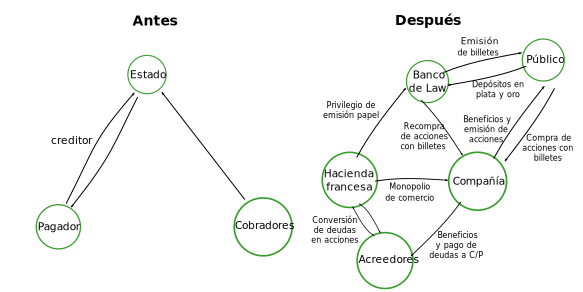
\includegraphics[width=150mm]{capitulos/graficos/grafoMercadoLaw} 
\label{fig:grafoMercadoLaw}

	\footnotesize
	Fuente: Elaboración propia a partir de Neal, \& Atack. (2.007)

\end{figure}

\subsection{Le Banque Générale}
El primer componente del sistema desarrollado por John Law, fue instaurar un banco nacional,  \emph{le Banque Générale}. Este banco tenía como objetivo, mediante la emisión de billetes, estimular la economía y enriquecer a todos aquellos que depositaban oro y plata a cambio de obtener dinero fiduciario. 

El banco nacional, se propuso inicialmente para crear una unión con la red financiera existente entre el ente recaudador de impuestos y el pagador de estos impuestos. Law propuso resolver el problema grave de pagos que atravesaba el Estado, pero la propuesta fue rechazada por el gabinete del regente en octubre de 1.715, ya que en ese momento el gobierno se enfrentaba a una gran crisis económica nacional que afectaba a todo país y no disponían ni de dinero ni de crédito. 

En cambio, en mayo de 1.716 y tras una serie de operaciones 	\footnote{Debido a una reacuñación de la moneda.}
, finalmente el gabinete aprobó un nuevo decreto por el que, el banco nacional recibió el monopolio sobre la emisión de billetes. A primera vista y con excepción de este privilegio, inicialmente el banco nacional no recibió ningún otro tratamiento especial. 

Para elevar el capital disponible del banco, Law realizó una oferta pública de 1.200 acciones a 5.000 libras cada una. De este modo, los suscriptores podían comprar acciones a cambio de ciertos tipos de deuda pública \footnote{En francés: Palanquillas d 'Etat.}. El banco era de carácter \emph{privado}, pero desde el principio Law adquirió una cuarta parte de las acciones y el rey otra cuarta parte. Si se realiza una comparativa con la situación actual, este banco se estructuró de manera muy similar a una empresa moderna con responsabilidad limitada.

Entre las características de funcionamiento del banco, está la celebración de una asamblea general dos veces al año, en la que los accionistas votaban en proporción al número de participaciones que poseían. En ellas también se gestionaban las ganancias y se anunciaban los pagos de los dividendos pertinentes.

Entre las actividades principales del banco se encontraban: los descuentos de letras, la venta de divisas, la captación de depósitos, la gestión de las cuentas corrientes y la emisión de billetes pagaderos en monedas de oro a petición del portador. Aunque el banco era aparentemente una empresa privada, el Estado estuvo involucrado desde el principio a través de las participaciones que poseía el rey. La emisión de moneda fiduciaria, también fue un híbrido entre lo privado y lo público. El activo inicial del banco era la deuda pública. Los accionistas del banco eran acreedores del gobierno a los que se les dio la oportunidad de convertir sus obligaciones en acciones. 

Repartir billetes y que éstos no regresasen constantemente al banco, era el atractivo fundamental para la rentabilidad de éste. Hay tres factores que jugaron a su favor. El primero es que el regente y los partidarios influyentes y adinerados, invirtieron grandes sumas de dinero a través de depósitos de oro y plata, por lo que a lo largo de las primeras emisiones de billetes se hicieron contra los depósitos. De este modo, las personas que habían invertido estaban dispuestos a mantener los billetes que recibieron y no redimirlos. El segundo factor, son los elementos de la propuesta original bancaria de Law que se introdujo. Y por último, es que a los billetes se les protegió de una forma parcial en cuanto al impuesto de \emph{señoraje}. Según Zuleta (1.995), se entiende \emph{señoraje} como el poder de compra derivado de la expansión monetaria, es decir, el aumento de la cantidad de dinero en términos reales o aumento nominal (incremento de M) dividido por el nivel de precios (P). Se puede comprobar a través de la siguiente ecuación: 

\begin{gather*}
	Se\tilde{n}oraje = (\Delta M)/P
\end{gather*}

El señoraje es por tanto, un \emph{recaudo} de poder de compra que beneficia a quienes emiten dinero, es decir, los bancos centrales y los bancos comerciales; o a quienes reciben ingresos o créditos derivados de este recaudo de poder de compra.

Retomando la situación de \emph{le Banque Générale}, los recaudadores de impuestos estaban obligados a canjear los billetes por oro o plata. En cambio, en abril de 1.717, los billetes se convirtieron en moneda de curso legal en el pago de impuestos. En septiembre del mismo año, se ordenó a contables y cajeros fiscales del gobierno, que intercediesen para proceder a una correcta recaudación y realizar otros cobros y pagos en billetes. 

El banco obtuvo un rápido éxito a pesar de las dudas iniciales provocadas por el ambiente de incertidumbre que se vivía entre la población. Se emitió una cantidad elevada de billetes, entre cuarenta y cincuenta millones al año de media. Ante esta emisión de billetes tan desproporcionada, era imposible respaldar tan alta cantidad de dinero con reservas de oro y plata. Por ello, se ofrecieron servicios \emph{especiales} para el Estado y para los inversores \emph{importantes}.

Los pagos de dividendos\footnote{Tres pagos semestrales desde 1.716 hasta 1.718.} totales del banco nacional ascendieron a un ritmo del 15 por ciento sobre el precio al contado de las acciones iniciales. Los beneficios para los accionistas incluyeron una ganancia de capital considerable. En enero de 1.718, se presenta una revalorización de casi el 90 por ciento sobre el precio de compra con respecto a un año y medio antes \footnote{Se supone una acción pagada con 1/4 de efectivo y 3/4 billetes d'Etat a un 60 por ciento de interés.}. Tras el éxito que tuvo la creación del dinero papel, John Law dio un paso desconcertante y nacionalizó el banco. Esta nacionalización se dio en mayo de 1.718 tras dos años de actividad de éste. La Corona, compró con efectivo la totalidad de las acciones existentes a valor nominal\footnote{5.000 libras.}. A partir de este momento, el banco sería gestionado por Law en nombre del rey y todos los beneficios serían entregados a las arcas reales. 

La nacionalización del banco tuvo dos consecuencias:
\begin{enumerate}
	\item La primera de ellas plantea una cuestión: \emph{¿Cómo sobrevivió el crédito del banco a la nacionalización?} Tres años atrás, hubiese supuesto un completo fracaso, pero en 1.718 el gobierno del regente del rey se encontraba en una posición diferente, hasta entonces el gobierno había logrado traer un poco de orden a las finanzas públicas, con una gran variedad de medios tradicionales \footnote{Como por ejemplo, los impuestos sobre especuladores de la guerra, el señoreaje, aumentos de impuestos.}, así como la introducción de mejores prácticas de contabilidad.
	\item Por otra parte, el poder del Regente se había consolidado, porque había ganado un enfrentamiento con el Parlamento de París sobre la reacuñación de la moneda en mayo de 1.718 y se distribuyó con un complejo sistema de comités ocupados por figuras dominantes de la corte y del ejército. El regente y Law, se preparaban para la acción más audaz llevada a cabo en la reforma de Law.
\end{enumerate}


\subsection{El mercado financiero}

A continuación, se va a proceder a dar una amplia explicación de lo que provocó este cambio en el sistema financiero.

Como se puede observar a través de la Figura \ref{fig:grafoMercadoLaw}, \emph{le Banque Générale} dirigido por Law tenía el privilegio de emitir billetes a cambio del depósito de metales. Así, la gente que estaba dispuesta a invertir, depositaba la plata y oro, y a cambio aceptaba recibos o billetes 	\footnote{En francés: billets etat.} Para que los ciudadanos en un principio aceptasen estos billetes, la Hacienda francesa tuvo que aceptar el pago de impuestos con la nueva moneda fiduciaria. A su vez la Compañía del Mississippi, explicada en el punto 3.2.3, se hacía cargo de las deudas de la Corona. Estas deudas, las pagaría la Compañía con la corriente de ingresos de sus actividades monopolísticas. De este modo, la Compañía adquiría capital suscrito en la moneda fiduciaria a través de los nuevos accionistas, que éstos a su vez debían ir al Banco de Law para poder obtenerlas depositando oro y plata. 

Otra de las bases del sistema, era la manipulación de la cotización. El \emph{Banque Générale}, recompraba las acciones con billetes que él mismo emitía. Estas recompras se hacían a un precio superior provocando así, importantes ganancias de capital para los entonces accionistas. De este modo, lograron atraer a los inversores para adquirir más acciones de la Compañía Mississippi. La segunda ampliación tuvo un coste por acción suscrita tres veces más cara que la primera. Se pusieron altas expectativas en la Compañía, despertando aún más el interés de la ciudadanía por adquirir nuevas acciones, provocando una euforia entre los inversores. 

En un primer momento, la nueva moneda fiduciaria fue más aceptada que los metales como el oro y la plata. Este hecho se debió al interés suscitado por los inversores por adquirir acciones de la Compañía. Lo que supuso que esta emisión de moneda recayese sobre el Banco de Law ya que poseía importantes reservas de plata. 
El siguiente paso, fue fusionar el Banco de Law con la Compañía del Mississippi para disponer de un único punto de emisión de billetes y una única  reserva de plata. 

El ingenio de John Law permitió que se desarrollasen innovaciones financieras cómo las opciones de compra. Estas novedosas opciones de compra fueron usadas en los momentos álgidos de la burbuja, cuando parecía excesivo el ritmo de emisión de acciones pero seguía habiendo demanda de las mismas. 

Law aprovechó la situación para ordenar la emisión de nuevas acciones de la Compañía. Lo que supuso el préstamo de importantes sumas de dinero a la Corona, captando así, grandes cantidades de capital. Esto fue gracias al interés que la gente tenía por adquirir acciones aunque el precio de éstas fuese muy elevado. Mientras tanto, los inversionistas adquirían nuevos billetes procedentes del Banco de Law, a cambio de depositar oro y plata. El sistema era insostenible, ya que la Compañía del Mississippi era incapaz de remunerar a sus accionistas debido a las exageradas expectativas de rentabilidad. Llegado este punto, dos sucesos podían quebrar el sistema: 

\begin{enumerate}
	\item Una retirada masiva de fondos del banco. 
	\item Un pinchazo en la burbuja. De esta forma, los accionistas se percatarían de que no había renta suficiente para remunerar todo el capital empleado.
\end{enumerate}

En este segundo caso, la moneda fiduciaria caería estrepitosamente. Se alcanzaría un punto en el que ningún inversor estaría interesado en seguir adquiriendo acciones y como consecuencia, todos ellos acudirían en masa a recuperar sus fondos en forma de plata y oro. 

En definitiva, se puede concluir que se procedió a una importante liquidación de deudas. Se sustían así obligaciones en especie por acciones con un rendimiento por dividendo muy bajo pero con un potencial de revalorización muy importante provocado por la burbuja económica. 

A continuación, en la Figura \ref{fig:billeteJohn}, se muestra la única copia escaneada, que ha sobrevivido, de los primeros billetes de el \emph{Banque Générale}. Data del de 10 de junio 1.718. En él se puede leer el texto en frances: \emph{La Banque promet payer au porteur à veüe Cinquante Ecus d'Espèces, du poids et titre de ce jour, valeur receüe à Paris le 10 Juny 1718'}. La traducción al castellano es: \emph{La Banca se compromete a pagar al portador la especial cantidad de 50 coronas de especies. A día de hoy, valor recibido en París el 10 de Junio de 1.718}.

\begin{figure}[!h] 
\caption{Billete de 1.720 del Banque Générale} 
\centering 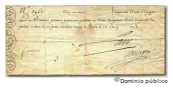
\includegraphics[width=50mm]{capitulos/img/billeteJohn} 
\label{fig:billeteJohn} 

	\footnotesize
	Figura recuperada de Wikipedia

\end{figure}

\section{La Compañía del Mississippi}
El siguiente movimiento del nuevo sistema de Law, fue la creación de la Compañía del Mississippi. Junto a esta Compañía, el banco nacional adquirió una mayor importancia.

A principios de 1.717, un conjunto de comerciantes y proveedores estaban desarrollando una gran colonia en Luisiana, que abarcaba toda la cuenca del río Mississippi. El territorio había pertenecido a Francia durante más de cuarenta años, pero hasta ahora nadie había percibido un rendimiento de él. Law se hizo cargo del proyecto con la aprobación del gobierno y lo hizo mucho más ambicioso, creando la Compañía de Occidente	\footnote{En francés: Compagnie d'Occident.} en agosto de 1.717.

La creación de la Compañía supuso la implantación de dos modelos. Uno de ellos, fue el del desarrollo de la tierra en el \emph{Nuevo Mundo}. De este modo, el gobierno entregó el territorio a la Compañía de Occidente pero sin que supusiese la pérdida de soberanía nacional, y a su vez, el gobierno esperaba beneficiarse de su desarrollo privado a través de la recaudación de impuestos. El segundo modelo a implantar, consistía en convertir deuda pública en acciones de la Compañía. Estas acciones eran potencialmente más arriesgadas, pero también más beneficiosas porque se repartía una mayor cantidad de dividendos.

Este último movimiento había supuesto un incremento de seis millones libras mientras que el valor de la Compañía se incrementó en 100 millones de libras. De hecho, la oferta de acciones comenzó el 14 de septiembre de 1.717, pero no se cerró hasta el 16 de julio de 1.718 debido al gran éxito. Una vez cerrada la operación, se tomaron medidas para acelerar el pago de la suscripción de las acciones, ya que todo el capital invertido no tenía el respaldo de las reservas de metales tales como oro y plata. Esto era debido a la emisión excesiva de billetes como moneda fiduciaria, en particular mediante la introducción de un sistema de pre-pago\footnote{Un accionista pagaba el 20 por ciento del precio y el resto lo paga en cinco meses, de lo contrario perdía el pago inicial.}. 

La suscripción se prolongó durante un largo periodo de tiempo, en parte, debido a la reclamación que los acreedores hicieron sobre el Estado, tal y como se podrá comprobar en la Figura \ref{fig:preciosAccionesIndias}. Esta reclamación, tenía su fundamento en el intercambio de bonos por acciones, ya que los intereses sobre los bonos era del 4 por ciento y fueron asignados sobre una explotación de impuestos. En julio de 1.718, la empresa propuso hacerse cargo de la explotación de tabaco beneficiándose de importantes sumas de dinero que posteriormente iban destinadas a las arcas estatales.
En un principio, el beneficio fue de cuatro millones de libras, exactamente la suma que el gobierno tendría que pagar a la empresa en concepto de intereses de los bonos de los suscriptores. Aun así, Law creía que podría funcionar mejor el monopolio esperando generar entre seis y ocho millones por año, una expectativa razonable, como se podrá comprobar a continuación.

Law se hizo cargo de los activos que provenían de Louisiana, incluyendo un barco para el que John Law contrató a personal competente y bien formado. Así, procedió a comprar, arrendar y construir nuevos buques, por lo que para diciembre de 1.718 la compañía tenía una docena de barcos a su disposición y ya se habían realizado con éxito varios viajes a Louisiana.

Al mismo tiempo, la Compañía creció debido a una serie de fusiones. Tras la concesión del monopolio del tabaco, la compañía compró otras sociedades mercantiles como la \emph{Compañía del Senegal} en diciembre de 1.718; la \emph{Compañía de las Indias}; la \emph{Compañía de China} y la \emph{Compañía de África} en junio de 1.719; la \emph{Compañía de Santo Domingo} y el monopolio de \emph{esclavos} en Guinea en Septiembre de 1.720. Esta situación concedió a la empresa el monopolio efectivo en casi todo el comercio de ultramar francés. La compañía también amplió sus actividades recaudatorias al sector agrícola en Lousiana creando los contratos de arrendamientos en julio de 1.719. Este tipo de contrato se denominó \emph{Granjas Generales} \footnote{En francés: Fermes Générales.} y en él, quedaba patente la obtención del permiso de recolecta de la mayor parte de los impuestos al consumo en Francia, a su vez, éste suponía un 30 por ciento de los ingresos del gobierno. Finalmente, a la Compañía se le concedió también el monopolio de recaudación de todos los impuestos directos\footnote{En francés: Recettes Générales.} de Francia, lo que suponía alrededor del 55 por ciento de los ingresos totales del país. En este momento, la Compañía del Mississippi pasó a denominarse como la Compañía de las Indias

Durante las primeras adquisiciones de otras compañías, la del Mississippi se fue financiando con activos iniciales de la empresa, pero la gran mayoría del resto de adquisiciones fueron financiadas con emisión de nuevas acciones. Cada nueva acción tiene igual jerarquía que las acciones antiguas, aunque la oferta aumentó con el transcurso del tiempo. La emisión inicial de fue de 200.000 acciones y se ofrecieron a 500 libras cada una, a pagar en bonos del gobierno a su valor nominal, es decir, en vez de con moneda fiduciaria, con reservas de oro o plata. En junio de 1.719 se realizó una nueva ampliación de capital de 50.000 acciones que se ofrecieron a 550 libras. En julio de 1.719 se ofertaban 50.000 acciones a 1.000 libras cada una. Y por último, en septiembre y octubre de 1.719 se amplió capital por 300.000 acciones a 5.000 libras cada una. Todas las ampliaciones de capital se debían de pagar en efectivo, es decir con reservas de oro y plata. 

De este modo, la segunda y tercera ampliación de capital, tomaron la forma de una oferta de derechos, es decir, un suscriptor de la ampliación de junio tuvo que poseer cuatro acciones originales o \emph{madres} y un suscriptor de la edición de julio tuvo que poseer cuatro acciones \emph{madres} y una acción \emph{hija} para poder comprar una acción \emph{nieta}. Este requisito provocó un mayor frenesí suscriptor  entre la población francesa.

Después de realizar el pago de las acciones, el accionista recibía un certificado por el que le daba derecho a una participación en el pago total de todo el desembolso. Esta característica, señaló Cochrane (2.001), cuando los pagos eran reembolsables, la suscripción era la primera norma. Esta función también caracterizó en la cuarta suscripción, generalmente llamada \emph{sumisión}. 


\section{La evolución de precios y el estallido de la burbuja}  
Hay que tener en cuenta dos aspectos fundamentales. El primero es que la burbuja económica no surgió espontáneamente, y el segundo, es que el nombre asignado a la burbuja en castellano no es tan revelador como el nombre en francés: \emph{Le système de Law}\footnote{En castellano podría traducirse como \emph{El sistema de Law}.}.

Sea como fuere, hay que ser conscientes de que la burbuja económica surgió gracias al manejo del mercado de John Law sobre la Compañía y sobre el propio mercado. Vale la pena señalar que, si bien la Burbuja de los Mares del Sur de Londres fue testigo de una proliferación de sistemas y empresas y un aumento sustancial en el mercado de acciones, en contraposición se encuentra la burbuja francesa que tan sólo concierne a una sola empresa \footnote{Parte del esquema de Law era comprar otras empresas comerciales, para sacarlas del mercado y obtener así el monopolio}. Law gestionaba activamente el mercado y el aumento de precios del mismo. Tal y como refleja Herbert Lüthy (1.961) en su obra: \emph{La Banque protestante en France de la rèevocation de l'Édit de Nantes á la Rèvolution}, Law había estado influyendo o manipulando el precio de las acciones de su compañía durante un largo periodo de tiempo, esto fue posible gracias a la adquisición de nuevas empresas para conseguir el monopolio.

Como desarrollo del segundo punto, cabe decir que la Compañía estaba acumulando una gran colección de Compañías rentables. El aumento de precio en las acciones de la Compañía del Mississippi refleja el hecho de que estas nuevas compañías comerciales adquiridas por Law, se convirtieron también a su vez en acciones. 

La prehistoria de la bolsa francesa no es bien conocida. En la Edad Media, los operadores de divisas en París se reunían en el llamado \emph{puente de intercambio} \footnote{En francés: Pont au Change}, cerca de la Casa de Moneda. A finales del siglo XVI los cargos oficiales fueron creados, pero no había un lugar oficial donde se reuniesen.

Cuando la compañía de Law estableció sus oficinas en la \emph{rue Quincampoix}, significó la creación de un punto local para este tipo de mercado. En ese momento el mercado se había vuelto visible. Finalmente, el gobierno decidió reconocer y regular el mercado y le dio un lugar permanente en septiembre de 1.724.

Law no sólo había creado el mercado en un sentido físico, sino que también presentó a la población francesa los tipos de instrumentos financieros conocidos por los comerciantes holandeses e ingleses. En 1.718, la suscripción de la Compañía de Occidente languidecía en el momento en el que Law anunció\footnote{Anuncio publicado en la Gaceta d'Amsterdam el 23 de mayo de 1.718.} públicamente su disposición a comprar acciones de la Compañía de Occidente a cambio de una prima del 2 por ciento. El emisor de la opción se comprometió a la entrega de una acción en cualquier momento del año siguiente en el que Law eligiese, al 70 por ciento de su valor nominal. Esta afirmación, garantizaba al accionista 100 libras en lingotes de oro del Estado, el dividendo mínimo del 4 por ciento en la participación y el porcentaje de la prima correspondiente a la ampliación de capital número dos.

Pero es en el otoño 1719, tras la conversión de la deuda y después de que la Compañía se convirtiese en un participante activo del mercado, cuando el precio de las acciones se fue mermando.

\begin{figure}[!h] 
\caption{Precios de las acciones de la Compañía de las Indias} 
\centering \includegraphics[width=150mm]{capitulos/graficos/preciosAccionesIndias} 
\label{fig:preciosAccionesIndias} 

	\footnotesize
	Fuente: Thornton, H (2.010)

\end{figure}

El 28 de agosto de 1.719, y tal como se puede apreciar en la Figura \ref{fig:preciosAccionesIndias}, la deuda del estado convertida en acciones, había estado avivando el precio de las acciones de 3.100 libras a 3.500 libras. Una ampliación de capital por valor de 500 millones de libras se había anunciado la noche del 14 de septiembre del mismo año, cuando los precios de las acciones se situaban en las 5.000 libras. En un plazo de tres días, las acciones ganaron otras 300 libras. Tras estas repentinas subidas de precios, éstos comenzaron a caer por en la segunda quincena de septiembre situándolo debajo de las 5.000 libras. 

A finales de octubre se tenía que efectuar el primer pago mensual, por parte de los suscriptores, correspondiente a las primeras suscripciones. Pero un decreto del 20 de septiembre consolidó los pagos mensuales en pagos trimestrales y aplazó el primero a diciembre.

La segunda ampliación de capital, se anunció el 30 de septiembre porque las acciones cayeron a 4.100 libras. El 2 de octubre, los precios alcanzaron las 4.335 libras pero al día siguiente cayeron de nuevo a 4.200 libras cuando se anunció la tercera emisión de 500 millones de libras.

El manuscrito de \emph{Giraudeau} coincide con la Figura \ref{fig:preciosAccionesIndias}, y muestra como el precio de las acciones volvió a incrementar situándose en 4.500 libras el 4 de octubre. Para los días 5 y 6 de octubre, las acciones cayeron a 3.800 libras, lo que produjo la convocatoria, por parte de Law, de una reunión con los directores de la empresa. Al día siguiente, el precio de las acciones al comienzo del día, sufrieron un aumento hasta alcanzar las 4.000 libras y se cerró en 4.250 libras. Ese mismo día, el 5 de octubre, el \emph{Banque Générale}, anunció que estaba dispuesto a comprar acciones a 4.500 libras y al día siguiente las acciones escalaron hasta esa cantidad, lo que provocó que el 7 de octubre ascendiesen a 4.750 libras.

El 13 de octubre, el banco todavía estaba comprando acciones a ese precio y el mercado se situó apenas por encima de las 4.500 libras como se puede apreciar en la Figura \ref{fig:preciosAccionesIndias}. Un real decreto del 12 de octubre, en alusión explícita a los rumores de nuevas emisiones de acciones, se comprometió formalmente a que ninguna de las otras acciones se iba a vender de manera diferente a la establecida anteriormente. A la semana siguiente, las acciones subieron a 4.900 libras.

Otro episodio de caída de precios tuvo lugar en diciembre de 1.719. El problema fue una crisis de liquidez debido a la cercanía de la fecha límite para hacer los pagos de las suscripciones. Cabe destacar que las suscripciones son opciones sobre acciones y que para mantener viva la opción, el dueño tuvo que realizar pagos periódicos. El decreto del 20 de septiembre, anteriormente mencionado, permitió que el precio de la acción se situase en 6.000 libras	\footnote{El periódico \emph{Amsterdamse Courant} irónicamente señaló que el mercado está liderado por los sucesivos decretos cual orquesta que bien podría llegar a saltarse toda una octava.}. A finales de diciembre, se debía realizar el primer pago por parte de los suscriptores, ya que no se efectuó en septiembre y la suma ascendía a 1.500 libras.

Los especuladores, tal y como se puede observar en la Figura \ref{fig:preciosAccionesIndias},  comenzaron a vender algunas suscripciones para financiar el pago de las demás, y esto llevó a la bajada de precios desde un máximo de 9.525 libras, el 2 de diciembre a 9.250 libras, el 9 de diciembre. A continuación, el 14 de diciembre, los precios se desplomaron a 7.430 libras. Del mismo modo, los derechos de suscripción cayeron de 5.700 libras el 2 de diciembre a 3.000 libras el 14 de diciembre. Ese día, el banco volvió a intervenir mediante la publicación de un precio de compra de 4.000 libras, y por la noche las suscripciones aumentaron de precio nuevamente a 4.500 libras. Sin embargo, la empresa mantiene el calendario vigente para el pago inicial de la suscripción. El siguiente rumor, fue la proximidad de la asamblea general de accionistas del 30 de diciembre. Las acciones originales llegaron a su máximo histórico el 23 de diciembre, cuando alcanzaron las 10 000 libras.

A lo largo de este período, el banco también prestó 2.500 libras al 2 por ciento anual, poniendo en peligro la seguridad del precio de la acción\footnote{La acción estaba respaldada por las reservas de oro y plata.}. Este hecho,  provocó una bajada en el precio de la acción y fomentó la especulación con el incentivo del \emph{dinero fácil}. La cantidad de dinero prestada ascendió a 276 millones de libras.

El 30 de diciembre de 1.719, en la Asamblea General, se decidió abrir una oficina en la que las acciones y las suscripciones pudieran ser compradas y vendidas para los precios publicados cada día. Esta oficina funcionó de manera intermitente, cerrándose entre el 10 y el 15 de enero, y abriendo sus puertas de nuevo a partir del 29 enero y hasta el 10 febrero. Por último, el precio de las acciones el 5 de marzo, se fijaron en 9.000 libras. En mayo de 1.720, la empresa había comprado 800 millones de libras en acciones, alrededor del 16 por ciento de su capitalización, con adición de emisión de moneda fiduciaria.

A partir de enero de 1.720, ya no se pudo considerar el precio de las acciones como \emph{precio de mercado}. El mercado se puede controlar si no existen manipuladores, pero como ya se ha mencionado, la manipulación del mercado por parte de Law, era una característica crucial de este sistema financiero con el fin de que el precio de las acciones siguiese al alza. En agosto de 1.719, la conversión de la adquisición de las compañías comerciales en acciones fue una catástrofe a largo plazo para la Compañía del Mississippi y para el gobierno, dando lugar así, a un precio ficticio de las acciones.

La manipulación del sistema tuvo consecuencias desastrosas para John Law, ya que probablemente se dio cuenta de que existían grandes incoherencias y trató de subsanarlas desarrollando una serie de políticas financieras entre finales de febrero y principios de marzo de 1.720. 

El 22 de febrero de 1.720, La \emph{Banque Générale} se fusionó con la Compañía con la intención de impedir crédito a la Corona. El efecto sobre los precios fue inmediato como se puede comprobar en la Figura \ref{fig:preciosAccionesIndias}. De 9.425 libras el 22 de febrero a 8.000 libras el 1 de marzo, mientras que el precio de las suscripciones se redujo de 6.600 libras a 5.450 libras. La reacción de Law fue inmediata ya que retrocedió unos pasos en cuanto al precio de las acciones se refiere. El 5 de marzo, se abrió otra oficina para la compra y venta de acciones a un precio fijo de 9.000 libras. Al mismo tiempo, las suscripciones pendientes perdieron sus opciones y fueron convertidas en acciones a una proporción de 2 por 3, mientras que los reembolsos de la deuda pública se siguieron realizando, pero en billetes del banco. Desde marzo hasta finales de mayo de 1.720, la compañía pasó otros 1.319,5 millones de libras a dinero papel para comprar el 28 por ciento de sus acciones, lo que supone un aumento colosal en cuanto al valor de la compañía.

El desastre ya se estaba gestando. Law fue obligado por el Consejo del Rey a controlar la oferta monetaria nominal, bien reduciendo un gran número de billetes en circulación o mediante la reducción del nominal de cada billete. Como se puede observar en la Figura \ref{fig:preciosAccionesIndias}, el 21 de mayo de 1.720, la confianza de los compradores llegó a su fin provocando el estallido de la burbuja económica. Entre junio y agosto de 1.720, se tuvieron que recomprar los billetes y las acciones con la moneda antigua. Realizándose así el 15 de agosto, una desmonetización gradual de los billetes. En noviembre de 1.720, el experimento monetario de John Law había finalizado y la compañía de Law era declarada insolvente. Law fue al exilio el 18 de diciembre.

Con la siguiente Figura \ref{fig:ComparaMississippiMaresSur}, se va poder observar los precios alcanazados por la Compañía del Mississippi y por la Compañía de los Mares del Sur, explicada en el capítulo que viene a continuación.

\begin{figure}[!h] 
\caption{Comparación de precios de las acciones entre la Compaía del Mississippi y la Compañía de los Mares del Sur} 
\centering 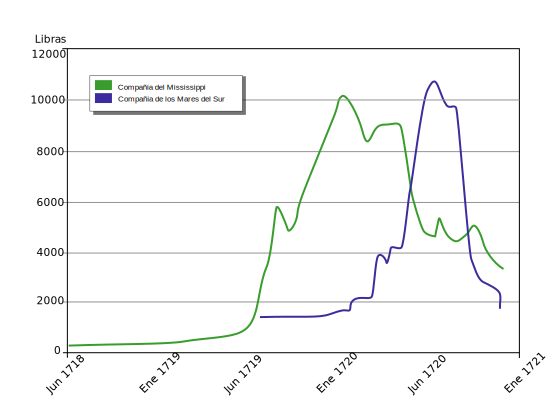
\includegraphics[width=150mm]{capitulos/graficos/ComparaMississippiMaresSur} 
\label{fig:ComparaMississippiMaresSur} 

	\footnotesize
	Fuente: William Goetzman (2.010)

\end{figure}



\chapter{La burbuja de la Compañía de los Mares del Sur}
\section{Contexto histórico}

La burbuja de los Mares del Sur coincidió con el rápido desarrollo de los mercados financieros en Europa a finales del siglo XVII y principios del XVIII. Este período vivió la introducción de un mercado secundario activo tanto en deuda como en renta variable. 

Se ubica el nacimiento de la Compañía de los Mares del Sur en el año 1.711 de la mano de Robert Harley. La situación del gobierno inglés por aquel entonces no era estable y necesitaba sanear sus cuentas de un modo sencillo y rápido. Se creyó que una brillante forma de llevarlo a cabo sería poniendo en marcha el comercio con América del Sur. Este mercado consistiría en la recolecta de metales preciados y pieles entre otros productos, por los que en Europa se obtendrían grandes beneficios.

El mayor problema era que Inglaterra estaba en guerra con España y ésta poseía el control de casi todos los países suramericanos. Pero en 1.713, se dio por finalizada la Guerra de Sucesión Española, e Inglaterra pudo comenzar a comerciar con América del Sur, si bien de una forma muy limitada, hasta que en 1.718 volvieron a enfrentarse en una nueva guerra donde Inglaterra salió victoriosa. Un año más tarde, los ingleses se hicieron con parte del control del mercado con América del sur. De este modo, la Compañía de los Mares del Sur se vio reforzada contando con barcos de esclavos y barcos textiles que navegaban bajo la bandera de la Compañía. Aun así, desde sus inicios, la Compañía estaba más involucrada en subsanar los problemas de la deuda, tema que se tratará con más detalle a lo largo del capítulo. 

\section{Surgimiento de las cofee houses}

Los comerciantes del siglo XVIII y los inversores tuvieron que depender en gran medida de las \emph{coffee houses}, es decir, las cafeterías, y también de la prensa para obtener información acerca de las inversiones y de los movimientos del mercado. Estas dos fuentes de información eran interdependientes, ya que los periodistas obtenían gran parte de sus informaciones en estas cafeterías.

Después de 1.695, los medios de comunicación comenzaron a desarrollarse proporcionando una gama cada vez más amplia de publicaciones para su clientela. Por su parte, las cafeterías en Londres proliferaron a partir del siglo XVI y en el año 1.700 había más de 2.000, convirtiéndose no sólo en un lugar de ocio, sino en una biblioteca donde las revistas podían ser estudiadas por un público ávido de noticias, lo que supuso una revolución en los hábitos sociales y de ocio de la población. La clientela inicial que frecuentaba las cafeterías, era de carácter selecto, por ejemplo casas literarias, sabios eruditos, políticos y abogados entre otros. Para llevar a cabo transacciones comerciales existían cafés especializados que atendían a las compañías marítimas y a empresas de seguros de vida.

Una de las funciones más destacables de las cafeterías es que eran una fuente muy importante de información política, económica y financiera. En efecto, antes de que existiese la libertad de prensa eran probablemente la principal fuente de noticias.

\section{La compañía de los Mares del Sur}

Hay que destacar la semejanza, que en un principio, podrían mostrar las dos situaciones financieras, tanto la de Inglaterra como la de Francia. Al desarrollarse en primer lugar la de la Compañía del Mississippi, es inevitable destacar la influencia de la teoría del dinero y el sistema desarrollado por John Law. El gobierno inglés se percató de que atravesaban una situación similar a la francesa, es decir, se estaban buscando alternativas a la resolución de su deuda pendiente acumulada, y su planteamiento era un esquema similar a la operación del Mississippi que llevó a cabo Law. 

Por otro lado, el primer director de la compañía compró deuda estatal en el año 1.719. Emitiendo así, acciones por las que se recibían dividendos todos los años. De este modo, Inglaterra lograba obtener liquidez para saldar deudas. 

Tras un proceso de licitación entre el Banco de Inglaterra y la Compañía de los Mares del Sur, esta última ganó el derecho a comprar 31,5 millones de libras en anualidades del Estado a largo plazo, a corto, e incluso deudas reembolsables. Las anualidades son ingresos periódicos de los que goza el comprador de la acción, bien a corto plazo o a largo plazo. En cambio, en las deudas reembolsables, la deuda es amortizable cuando en un momento determinado hay que pagar íntegro el capital. 

El gobierno accedió a adquirir el crédito de la Compañía ya que eso suponía un incremento en el presupuesto estatal de 31,5 millones de libras esterlinas. Así, ese nuevo capital se podía emplear para pagar las deudas adquiridas por el Estado. 

\section{Evolución de la burbuja económica de los Mares del Sur}

Algunos estudios han enmarcado a esta burbuja como un comportamiento irracional basándose en gran medida en anécdotas y citas contemporáneas. Contribuciones más recientes han tratado de explicar el aumento de la cotización de las acciones de la Compañía de los Mares del Sur en un marco racional.

Se ha de tener en cuenta, que los datos empleados en los últimos años, a la hora de analizar la burbuja de los Mares del Sur, nunca se habían tenido en cuenta en los estudios de la época. Los resultados ponen de manifiesto la falta de relación de los contratos a largo plazo y los precios se suscripción de las acciones de la compañía de los Mares del Sur.

Sin embargo, estos resultados dependen fundamentalmente de las fuentes de donde se colecten los precios de las acciones, los precios de suscripción y el tipo de interés al que los bancos prestaban dinero. Éstos, deben ser lo más fiables posible.

En contraposición, Garber (2.000) llega a la conclusión de que la burbuja de los Mares del Sur se puede comprender como un caso de especulación en la que los inversores trabajan sobre la base de los mejores análisis económicos disponibles y los precios empujan hacia el incremento a lo largo de su camino. Esto se debe a su visión cambiante de los fundamentos del mercado. Por esta razón, defiende la inexistencia de burbuja económica en la Compañía de los Mares del Sur.

\subsection{Tipos de contratos y análisis de precios}

Para realizar un correcto análisis, hay que recordar que las suscripciones son opciones sobre acciones que para mantener viva la opción, el suscriptor tuvo que realizar pagos periódicos. Por lo que se deduce que las acciones no se entregan inmediatamente. Por consiguiente, la fecha de liquidación era indefinida y el contrato con los suscriptores seguía vigente pero las entregas de las acciones todavía no se hacían efectivas. En consecuencia, había dos tipos de contrato en los abonos: 

\begin{enumerate}
	\item \emph{Mercado secundario}: Se trata de adquisiciones de acciones que ya han sido emitidas anteriormente en el mercado.
	\item \emph{Contratos forward}: Donde los compradores pagan por adelantado al precio actual de mercado con la previsión de contar con las acciones en un momento futuro determinado.
\end{enumerate}

Teniendo en cuenta estos contratos, se va a proceder a realizar un análisis de precios sustentado por autores relevantes.

En primer lugar, John Freke (1720), autor de la época, publica diferentes precios para las dos clases de contratos, es decir, para los contratos forward y para los contratos en mercados secundarios para la tercera y cuarta suscripción. 
En segundo lugar, según indica Freke, si en algún momento existe divergencia de precios entre los dos tipos de contratos, siempre usará como referencia el contrato forward.

Los estudios de Neal (2.009) dan una opinión acerca de la crisis de la Compañía de los Mares del Sur. Para este autor, no es más que una crisis crediticia que ocurrió en plena burbuja económica. Hay evidencia de que el Banco de Inglaterra prestaba líquido al 5 por ciento a lo largo de todo el período cubierto por el análisis, pese a que se llevan a cabo criterios más estrictos para los préstamos en las últimas etapas de la burbuja. 

Hutcheson (1.720), señala que algunos individuos estaban pagando tasas muy altas ya en abril de 1.720. Aun así, debieron ser más cuidadosos ya que se otorgaron préstamos a individuos sin capacidad crediticia lo que provocó que se asumiese un alto riesgo de incumplimiento de pagos. 

En resumen, la evidencia sugiere que el 5 por ciento es una tasa de descuento apropiada para el período en el que la burbuja perduró. 

Al analizar las cuatro suscripciones de dinero de una manera equitativa, el resultado es que ninguna sufre desventaja, ya que cada suscripción se limitó a presentarse como un medio para adquirir liquidez a través de un sistema de pagos escalonados, que varían para cada suscripción. Una vez descontados adecuadamente los pagos a plazos de las cuatro suscripciones, los valores y las suscripciones de acciones se convierten en instrumentos directamente sustituibles entre sí, ya que representan activos equivalentes y dividendos. En consecuencia, los precios de suscripción ajustados se pueden comparar directamente entre sí y también con el precio de las acciones. 

\input{./capitulos/tablas/pagosSuscripciones.tex}


Los datos de precios utilizados en el Cuadro \ref{tab:pagosSuscripciones} para la suscripción de acciones de la Compañía de los Mares del Sur, es del autor John Freke (1720).  Desde 1.714 hasta 1.722 redactó y publicó dos veces por semana una lista de precios de dicha Compañía. Cada publicación abarca tres días de negociación, es decir, de miércoles a viernes, y de sábado a martes\footnote{Se debe tener en cuenta que no hay comercio los domingos.}. Freke, se encargaba de recoger los precios de dados a lo largo de la mañana hasta las 15:00 horas de cada día. En ocasiones, incluye hasta tres precios por día, cuando este caso se produce, se realiza un promedio simple que proporciona un único precio para el día. 

Pese a que John Freke era conocido como un defensor de la Compañía de los Mares del Sur y su plan financiero, este hecho por sí solo, no debería ser suficiente para descartar su listado de precios, porque no se puede determinar si éstos sufrieron una distorsión sistemática o si este posible hecho podría haber favorecido a la Compañía. Freke actuaba como proveedor comercial de datos, por lo que era muy consciente de que cualquier percepción distorsionada de datos destruiría su negocio. 

Otra fuente de datos alternativa es la de Castaing (1.720) y su publicación \emph{El Curso de la Bolsa}, que comenzó a divulgarse en 1.697 y que poco a poco se convirtió en la lista oficial de precios de acciones de la Bolsa.

Sin embargo, la lista de precios de Freke se emplea más a menudo porque es más completa y representa una mejor fuente a la hora de proporcionar los mejores datos en una comparación detallada durante la burbuja de la Compañía de los Mares del Sur. Por ejemplo, los precios de suscripción que expresa Freke, no son cubiertos por Castaing, sobre todo en la tercera y cuarta suscripción. 

Ambos autores se encontraban en estrecha competencia. Aunque hay que matizar que la publicación de los informes de Freke, estaba dirigida al público londinense y en cambio el estudio de Castaing puede tener destinatarios diferentes, como pueden ser individuos no residentes de Londres, que tendrían un acceso más fácil al mercado de los recibos de suscripción.  Freke, y no Castaing, hace una distinción entre el \emph{precio actual} y los precios futuros de suscripción. Esto permite hacer una comparativa más directa de los precios de las acciones y la suscripción durante el período a estudiar. 

La serie más completa de los precios de Freke se encuentra en la Biblioteca Británica, aunque faltan los datos que abarcan desde el 21 hasta el 23 de mayo de 1.720. La lista completa de datos se maneja para proporcionar una serie continuada de los precios de las acciones de la Compañía y los precios de suscripción. Dichos datos comprenden el intervalo temporal del 14 de mayo de 1.720 al 27 de septiembre del mismo año, momento en el que la burbuja comenzó a deshincharse. En cambio, los precios de suscripción están completos hasta finales de 1.720, pero su valor para este estudio es cuestionable. Esto se debe a que a finales de septiembre, la Compañía de los Mares del Sur comenzó a estudiar medidas correctoras que implicaban el ajuste retroactivo de los dos últimos precios de suscripción. 

A continuación se van a mostrar dos gráficos. En el primero de ellos, que se corresponde a la Figura \ref{fig:precioSuscripciones}, se puede observar la serie de valores y los precios de suscripción para el período desde el 14 de septiembre hasta el 27 de septiembre del año 1.720

\begin{figure}[h!]
	\caption{Precio que alcanzaron las acciones en las suscripciones en el año 1720}
	\centering
	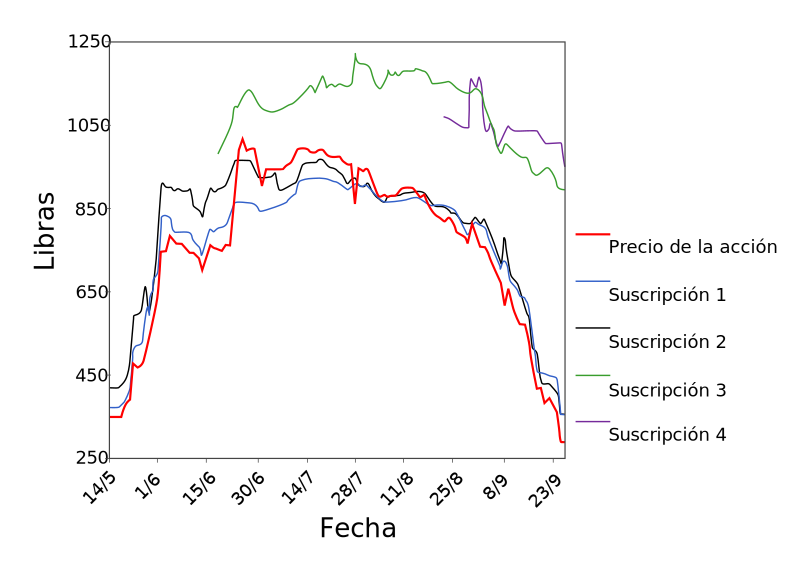
\includegraphics[width=150mm]{capitulos/graficos/precioSuscripciones}
	\label{fig:precioSuscripciones} 
	
	\footnotesize
	Fuente: Richard S. Dale, Johnnie E. Johnson \& Leilei Tang. (2.005)
	
	\raggedright
	\vspace{3 mm}
	Nota 1: Se ha utilizado la recopilación de datos de la Biblioteca británica que recogió Freke. Se ha de advertir que Freke no proporciona los precios de la suscripción número tres, es decir, del 18 a 21 junio. Por lo que los precios se han tomado son los de John Castaing. 
	
	\vspace{3 mm}
	Nota 2: Los días no comerciales, como los domingos, no se incluyen en el eje de fecha

\end{figure}

Según indican los autores de la Figura \ref{fig:tasaDeDescuento} Dale, Johnson y Tang, se puede apreciar el comportamiento irracional de la burbuja de los Mares del Sur. Esto es posible gracias a un índice que mide las tasas de descuentos que se dieron a lo largo de las cuatro suscripciones. Según el blog Gerencie, la tasa de descuento \emph{se utiliza para calcular el valor presente de los flujos de efectivo que se van a tener en el futuro; es decir los rendimientos que se esperan después de haber realizado la inversión}\footnote{Recuperado de Neira, N. (2008).}. De este modo, se puede establecer que la tasa de descuento debe corresponderse con la tasa de rendimiento requerida para los flujos de efectivo\footnote{ Según el Consejo Técnico de la Contaduría, se entiende que el flujo de efectivo \emph{es un estado financiero básico que muestra el efectivo generado y utilizado en las actividades de operación, inversión y financiación. Para el efecto debe determinarse el cambio en las diferentes partidas del balance general que inciden en el efectivo}. } que son los que determinan la capacidad de la empresa para generar efectivo. Es decir, con ella se determina el grado de cumplimiento de sus obligaciones y de sus proyectos de inversión y expansión que están asociados con la adquisición o inversión. Los factores mas importantes que hay que tener en cuenta a la hora de determinar esta tasa son: el tiempo, el mercado donde opera la empresa - en el caso que concierne a este capítulo, Compañía -, la situación política y económica del país y el sector bancario.

\begin{figure}[h!]
	\caption{Tipo de interés para los préstamos en las suscripciones}
	\centering
	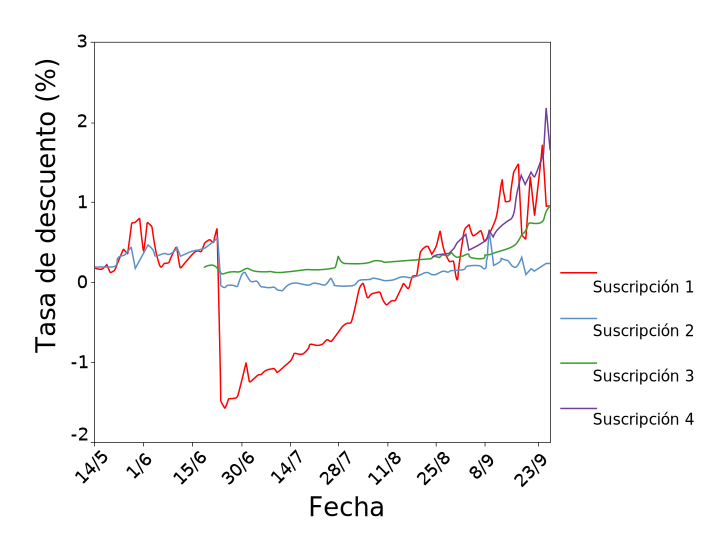
\includegraphics[width=150mm]{capitulos/graficos/tasaDeDescuento}
	\label{fig:tasaDeDescuento}

	\footnotesize
	Fuente: Richard S. Dale, Johnnie E. Johnson \& Leilei Tang. (2.005)

\end{figure}

\section{Evolución de los precios de las acciones y de las suscripciones}

La Compañía de los Mares del Sur se negó a fijar por adelantado el importe nominal de los valores canjeables\footnote{Según el blog Gerencie, los valores canjeables son \emph{los valores que pueden ser intercambiados por acciones ya existentes. No provoca ni la elevación del capital ni la reducción de las acciones}} por deuda. Cualquier aumento en el precio de la acción por encima del valor nominal provocaría una reducción de la cantidad necesaria para convertir la deuda pública pendiente. Por ejemplo, si el precio de la acción fuese 300 libras, la deuda pública de 31,5 millones de libras, podría ser comprada por la emisión de sólo 10.5 millones de libras en acciones. Los restantes 21 millones de libras de acciones emitidas, proporcionarían un posible flujo de efectivo de 63 millones de libras con el precio de mercado. 

No se dio salida al capital adicional recaudado en la emisión de acciones de la Compañía de los Mares del Sur. Este hecho, junto con el deseo de los accionistas de la Compañía de los Mares del Sur para conseguir ganancias de capital con su propia cartera de acciones, dio a la empresa un incentivo para lograr una apreciación sobre el precio de las acciones. Sin embargo, dicha valoración en el precio de la acción, proporcionó a la Compañía los medios para hacer que los dividendos se incrementasen. 

Además, se supo más tarde que en el intento por lograr la aprobación del Parlamento, la Compañía había propuesto \emph{opciones de compra}\footnote{O sobornos} a los ministros clave del gobierno y también a individuos influyentes que se encontraban estrechamente relacionados con la Corona. Este hecho proporcionó la seguridad necesaria a la Compañía a la hora de dar un impulso al precio de la acción.

A la hora de aplicar el sistema de conversión de la deuda, un escéptico miembro del Parlamento en ese periodo, lo describió como \emph{la gestión artística del espíritu del juego}. Una serie de estrategias fueron puestas en marcha para emitir más acciones, al tiempo que se maximizaba el precio de la acción de la Compañía:

\begin{enumerate}
	\item Cuatro emisiones de acciones sucesivas se ofertaron sobre los términos de suscripción generosos que implicaban tan sólo unos pequeños pagos iniciales.
	\item El guión fue diseñado para que la Compañía se mantuviese popular entre el círculo de los especuladores.
	\item Para aumentar la liquidez de los inversores y en consecuencia fomentar aún más la demanda de sus acciones, la Compañía de los Mares del Sur invitaba a los inversionistas a pedir prestado a la propia Compañía con la seguridad de que recibirían las acciones en el futuro. Más de 11 millones de libras fueron recaudadas de este modo.
	\item La Compañía de los Mares del Sur apoyó las subidas del precio de la acción mediante la compra de sus propias acciones.
	\item La compañía elevó las expectativas de los inversores, orquestando cuidadosamente los anuncios de importantes dividendos. Por ejemplo, en la víspera de la primera suscripción de dinero, que se produjo a mediados del verano, el beneficio por dividendo aumentó de un 3 por ciento a un 10 por ciento.
	\item La compañía tuvo que retrasar la emisión de acciones debido a que éstas se habían convertido en un motivo de rentabilidad. Así, no se pudo emitir recibos para la tercera y la cuarta suscripción. La intención de los directivos de la Compañía era hacer una ampliación de capital liberada \footnote{Según el centro de estudios financieros, se entiende la ampliación de capital social de una empresa como: \emph{La aportación de nuevos fondos a la sociedad, o bien de la capitalización de reservas. También puede se puede realizar una transformación de reservas a capital. Esto es posible mediante las ampliaciones de capital liberadas, en cuyo caso no se produce una entrada efectiva de fondos en la sociedad, si no que se trata de un mero apunte contable entre reservas y capital}.}y parcialmente pagada.
\end{enumerate}

Sin embargo, esta última estratagema era a lo sumo un éxito parcial, ya que los inversores podían suscribirse con total normalidad. Existen evidencias de que dichas negociaciones fueron llevadas a cabo finalmente. 

En este contexto, se puede ratificar que el precio de las acciones de la Compañía de los Mares del Sur, había avanzado desde las 130 libras en febrero de 1.720 hasta las 300 libras a principios de abril. Aun así, se continuó en esta línea de crecimiento, ya que en tan sólo once días sufrieron un incremento de doscientas libras. El 20 de mayo, el precio se situaba en 400 libras, el 28 de mayo alcanzó las 500 libras y se cerró el mes en 600 libras. Este ascenso gradual continuó el mes siguiente: el 1 de junio la acción se situaba en 700 libras y en tan sólo cuatro días aumentó cien libras alcanzando el valor de 800 libras por acción.

El 23 de junio, la empresa cerró sus libros contables durante dos meses con el fin de procesar debidamente todos los dividendos, por lo que los precios cotizados durante estos dos meses son los precios de contratos forward. Este tipo de contrato, es el más antiguo y se conoce también como \emph{contratos a plazo}. Esta clase de contrato obliga a sus participantes a comprar o vender un determinado activo en una fecha específica futura a un cierto precio\footnote{Recuperado de Zorrilla, J. P. (2010).}.

A la hora de realizar la apertura de los libros, el precio forward más alto registrado era de 1.050 libras del 25 de junio, pero cuando se reabrieron los libros, el precio al contado cayó a 820 libras. Así, la Compañía se encontró con que muchos de los que antes apoyaban sus estrategias, ahora pasaban a ser enemigos. Un claro ejemplo son los parlamentarios que exigieron la venta de parte de sus acciones al banco de Inglaterra. Aun así, el Parlamento perdonó una deuda de 7,1 millones de libras. 
Tras este desaire, el precio de las acciones de la Compañía de los Mares del Sur se debilitó drásticamente hasta descender a las 520 libras por acción, a mediados de septiembre y a 290 a principios de octubre. El mínimo se marcó el 14 de octubre de 1.720, día en que la burbuja estalló. 

\section{El banco de Hoare}
Para realizar un análisis acerca de la especulación producida a lo largo de la burbuja de los Mares del Sur, es interesante aportar un ejemplo de comportamiento comercial de un inversor sofisticado.

Este epígrafe va a dar una visión sobre las operaciones diarias de un banco propiedad de un orfebre, el Banco de Hoare. Aportando un punto de vista alternativo de cómo se puede inflar una burbuja económica a través de los registros efectuados por el propio banco. Estos datos proporcionan información sobre el tamaño del comercio, la frecuencia, el precio de ejecución, las pérdidas y ganancias, así como las órdenes que los clientes ejecutaron. 

\subsection{Historia del banco de Hoare}

El Banco Hoare era, y hoy en día continua siendo, un banco privado propiedad de la familia Hoare. Su fundador, Richard Hoare comenzó como un orfebre que trasladó su residencia en 1.690 a Londres, más concretamente a Fleet Street, donde poco después comenzó a concentrarse en la banca. El banco contaba con una larga lista de clientes de sangre azul. Entre los servicios ofrecidos por éste se encontraban los servicios de pago, los préstamos e inversión en carteras de valores, etc. También, negociaban activamente por su propia cuenta como si de autónomos se tratase. Los primeros libros de contabilidad datan de 1.702.

Desde la creación de la Compañía de los Mares del Sur, este banco invirtió en acciones de otras compañías como la \emph{Sociedad Real de África}, la \emph{Compañía de las Indias Orientales}, y el Banco de Inglaterra, así como las diversas la deudas públicas como se puede observar en el Cuadro \ref{tab:cuentaHoare}:

\begin{table}
    \begin{tabular}{lccccc}
                           & Número de        & Valor & Promedio      & Valor total & Inversión \\
                           & transacciones    & medio & de acciones   & en el       & máxima    \\
                           & en 1720          &       & en el mercado & mercado     &           \\ 
    \cline{2-6}
    Banco de Inglaterra    & 20               & 2.357 & 1.45          & 47.155      & 22.623    \\
    Compañía de las Indias & 7                & 3.423 & 1.071         & 23.96       & 14.990    \\
    Compañía de los        & 54               & 2.593 & 1.157         & 140.029     & 37.520    \\
    Mares del Sur          &                  &       &               &             &           \\
    \hline
    \end{tabular}
    
	\center
	\footnotesize
	Fuente: Charles Kindleberger (1.996)
	
    \caption {Actividad de mercado en la cuenta de Hoare en 1720}
	\label{tab:cuentaHoare}
\end{table}


La entidad financiera tuvo un éxito poco usual en su mercado. Según el estudio de Carswell (1.993), el beneficio en unidades monetarias reales ascendería a 7,1 millones de dólares. Mientras tanto, muchos inversores, algunos tan conocidos cómo Isaac Newton, perdieron importantes sumas de dinero en 1.720 debido a la burbuja económica. 

\subsection{Modelo simplificado del banco de Hoare}

Los autores Peter Temin y Hans-Joachim Voth (2.003), sostienen que en este episodio, el comportamiento de un inversor individual y su sabiduría, pueden decir mucho sobre la naturaleza de las burbujas y sobre el comportamiento de los inversores durante los periodos en los que surge una manipulación de precios. 

Tres puntos de vista a tener en cuenta debida su importancia son:

\begin{enumerate}
	\item El banco Hoare, no apostaba en contra del rápido crecimiento de la Compañía de los Mares del Sur, pero creaba indicios para que la población creyese que las acciones estaban sobrevaloradas.
	\item Era muy rentable para los participantes del mercado, ya que obtenían información de primera mano al unirse a la burbuja por un período prolongado antes de que se colapsase, en lugar de abandonar el mercado.
	\item No hay evidencias de que el banco Hoare invirtiese el dinero suficiente para comprometer la solvencia de éste. De acuerdo con el estudio teórico reciente de Abreu y Brunnermeier (2.003), parece que la necesidad de coordinación, para que la burbuja de los Mares del Sur se colapsase, fue la clave para permitir que ésta se inflase hasta el estallido. Además, el hecho de que los comerciantes racionales no lograsen evitar una burbuja era en realidad un síntoma de rentabilidad para ellos, como se refleja en los altos rendimientos obtenidos por Hoare en 1.720.
\end{enumerate}

A continuación, se va a presentar un ejemplo simplificado acerca del funcionamiento de este banco. Al ser un modelo tan abreviado no se ha de esperar dar respuesta a la totalidad de las preguntas sobre e funcionamiento de esta burbuja en concreto, pero puede arrojar luz sobre algunas de las cuestiones más importantes.

En 1.720, el banco negociaba de manera activa acciones de la Compañía de los Mares del Sur llevando a cabo cincuenta y cuatro transacciones y diecinueve operaciones destinadas a los clientes en ese mismo año. Sin embargo, tuvo su actividad máxima en las operaciones bursátiles de la Compañía. El banco, sigue un sistema de contabilidad doble y conserva un detallado registro de sus transacciones. Al igual que ocurre con las operaciones de crédito de los clientes. También se registraron las tasas de transferencia del costo total de las negociaciones. Las transacciones de los clientes abarcan los valores prestados contra la cantidad de acciones ofrecidas en garantía, la fecha de vencimiento y los intereses percibidos. 

En consecuencia, algunas de las operaciones que no estaban registradas en los libros de contabilidad, se llevaron a cabo en forma de recibos de contratos a plazos o suscripciones. En cuanto al comercio, éste fue eficiente la mayor parte del tiempo, cosa que benefició a todos aquellos en posesión de acciones o documentos de propiedad. Sin embargo, los suscriptores a menudo tuvieron que luchar con los procedimientos burocráticos diseñados para evitar una nueva suscripción de acciones. Solución que al parecer era mucho menos eficiente y eficaz que el comercio en sí. 

Los datos diarios y las pruebas fiables extremadamente detalladas de la posición del banco de Hoare, ayudan a obtener datos exactos para examinar el historial de operaciones del banco, y evaluar así, su rendimiento en comparación con el mercado y poder poner a prueba algunas hipótesis sobre el origen de su éxito. 

Para distinguir los diferentes argumentos sobre el auge de la burbuja de la Compañía de los Mares del Sur y del banco de Hoare, se describen tres situaciones que podía aportar a un inversionista en aquella época:

 \begin{enumerate}
\item Que el individuo fuese víctima de los impulsos irracionales y no de un análisis de mercado razonable. Por lo que los beneficios corrían a cargo de la suerte.
\item Que el comercio durante el tiempo en que tuvo lugar la burbuja se viese limitado por la seguridad del mercado. 
\item Que éste inversor actuase racionalmente, pero de un modo en el que favoreciese el desarrollo de la burbuja económica, es decir, comprando y vendiendo según el comportamiento esperado por los otros compradores y vendedores, es decir, siguiendo un comportamiento de \emph{herding}.
 \end{enumerate}

\subsection{El éxito del banco de Hoare}
\begin{figure}[h!]
	\caption{Comparativa del precio de las acciones de la compañía de los Mares del Sur y el mercado del banco de Hoare}
	\centering
	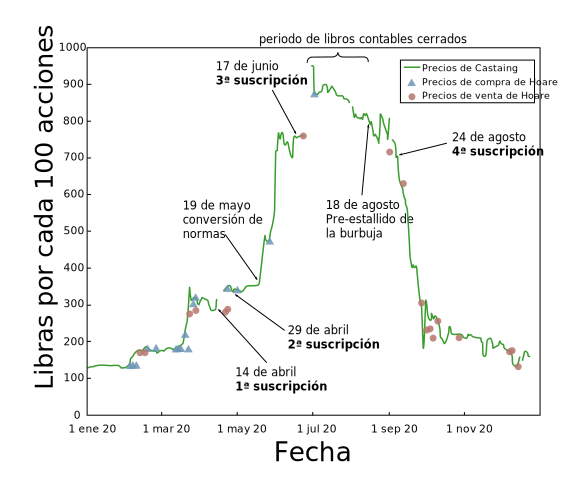
\includegraphics[width=150mm]{capitulos/graficos/bancoHoare}
	\label{fig:bancoHoare}

	\footnotesize
	Fuente: Peter Temin, \& Hans-Joachim Voth. (2.003)

\end{figure}

Como se puede comprobar en ella Figura \ref{fig:bancoHoare}, el Registro comercial de Hoare es sorprendente desde cualquier punto de vista, y este hecho no se debe al azar. Para demostrar que Hoare participó en la alimentación de la burbuja, también se ha de aclarar que el propio banco no se aprovechó de la ventaja del conocimiento de que las acciones de la Compañía de los Mares del Sur estaban sobrevaloradas. Obtener información privilegiada era sencillo ya que dentro de la larga lista de clientes del banco, muchos de ellos tenían buenos contactos que podrían haber proporcionado valiosa información.

Los clientes de Hoare que se sumergieron en el mercado durante este período fueron cruciales. En marzo de 1.720, \emph{Lord Carlton}, miembro del Parlamento, compró 6.000 acciones de la Compañía de los Mares del Sur que equivaldría a 9.000 libras que quedaron depositadas en el banco de Hoare. Éste último, a su vez había comprado 1.000 acciones el día anterior y otras 1.000 la semana anterior. A principios de marzo, pocos días antes de la transacción de Lord Carlton, el banco compró otras 7.000 acciones. Este hecho no sugiere que el banco estuviese acatando órdenes estipuladas por la Compañía de los Mares del Sur. La compra de Lord Carlton probablemente no era lo suficientemente potente como para que, sin ayuda externa, se lograse cambiar el precio de las acciones de la compañía de los Mares del Sur. Además, se ha de tener en cuenta que las compras especulativas en la Compañía de los Mares del Sur, antes del 17 de marzo, fueron muy comunes. El banco no llevó a cabo ninguna compra anterior al 21 de marzo, por lo tanto pagó el precio estipulado del 22 de marzo sobre 7000 acciones.

También hay algunas conexiones directas entre los clientes de Hoare y el pequeño grupo de iniciados que crearon la Compañía de los Mares del Sur. Sin embargo, ya que sólo se observa una información parcial a disposición de los comerciantes de la época, puede caber la posibilidad de que el éxito de Hoare derivase de que sus clientes conseguían una información privilegiada que les favorecía económicamente. 

El banco actúa normalmente como intermediario entre sus clientes y las compañías. En el caso del banco de Hoare, podía haberse beneficiado indirectamente de la certeza de que sus clientes eran conscientes de los hechos que se estaban sucediendo y de las decisiones que claramente iban a afectar al valor de las acciones. Los autores Gennotte y Leland (1.990), demuestran que, en condiciones generales, los participantes del mercado que siguen a las masas de individuos, tienden a actuar como inversores desinformados. Esto quiere decir que, compran cuando los precios descienden, y se venden cuando aumentan. Una vez que éstos reciben información precisa, por ejemplo mediante la observación de movimientos de las acciones de los inversionistas experimentados o por tener acceso a otra clase de información, sus decisiones sobre operaciones de liquidez comenzarán a tomar otro camino. En cuanto a las compras de acciones de la Compañía de los Mares del Sur, el comercio era similar. 

La combinación de los siguientes factores fue la clave el éxito del banco de Hoare. En primer lugar, la estrategia comercial por la que apostaron se basaba en la predicción de confianza de los inversores hacia las acciones durante la burbuja, apostando a que los precios subirían por un tiempo. En segundo lugar, el escenario en el que la burbuja de los Mares del Sur se desenvolvió. Es difícil distinguir entre el riesgo del comerciante y el \emph{riesgo de sincronización}8 de varios comerciantes. El riesgo de sincronización viene definido como \emph{la estrategia a la hora de realizar decisiones de compra o venta de activos financieros al tratar de predecir los movimientos futuros de los precios de mercado. La predicción puede basarse en una perspectiva de las condiciones del mercado o económicas resultantes de un análisis técnico o fundamental. Se trata de una estrategia de inversión basada en las perspectivas de un mercado global, en lugar de para un determinado activo financiero}. ¿Cómo se puede reducir este riesgo de sincronización? Primero se ha de analizar la actividad del inversor en busca de negociación excesiva. Y en segundo lugar, se debe emplear personal para examinar de modo selectivo y constante la actividad comercial reciente. Esta última, con el fin de identificar aquellas actitudes que puedan ser contrarias a esta política de negociación sobre sincronización con el mercado.

Según los autores Peter Temin y Hans-Joachim Voth (2.003), éstos establecen cinco conclusiones cómo consecuencia del comportamiento comercial del banco:

\begin{enumerate}
	\item El banco de Hoare era consciente de que existían inversores sin experiencia que se encontraban mezclados con los inversores especialistas. Según los datos del banco, los que dominaron la especulación son los inversores sin experiencia. Sin embargo, parecía rentable para la propia entidad mantuviese a estos inversores en el mercado.
	\item Las restricciones de venta de acciones a corto plazo, no influyeron de manera determinante en el desarrollo de la burbuja, puesto que el banco era propiedad exclusiva de los socios. Pero si fueron un problema los incentivos surgidos de las relaciones principales de los inversores con el banco. 
	\item Según la ficha comercial de precios por parte del banco, es poco probable que fuese impulsado por el conocimiento de información privilegiada por parte de sus clientes, y como consecuencia, afectase al comportamiento del banco comercial. 
	\item Tal y como está registrado en documentos de la época, los inversores podrían haber sido conscientes de que el precio de las acciones de la compañía de los Mares del Sur estaba sobreevaluado. 
\end{enumerate}

Por lo tanto, resumiendo estas cinco conclusiones, se puede decir que el sentimiento de previsibilidad es compatible con el \emph{riesgo de sincronización}.

Para finalizar este epígrafe, se ha de destacar como dato importante, la intención de medir la importancia e influencia económica que podría haber supuesto la extracción de información privilegiada por parte de la negociación de los clientes. Por ejemplo, si los rendimientos más altos son positivos, significa que siguieron las estrategias del banco de Hoare de comprar cuando los clientes compraban.

Se puede llegar a la conclusión de que el éxito comercial de Hoare no se puede explicar por la información inherente al comportamiento de la inversión de sus clientes.

\section{Sobrevaloración de las acciones}

Se conocen numerosos relatos del frenesí de la manía que explican como algunas doncellas y jubilados fueron engañados invirtiendo todos los ahorros de los que disponían en acciones de la Compañía de los Mares del Sur. Por todo lo que se mencionado a lo largo del capítulo y apoyando las teorías de autores contemporáneos, se puede ratificar que las acciones de la Compañía de los Mares del Sur sí se encontraban sobrevaluadas.

Los detalles del plan de conversión de deuda y las implicaciones exactas de las suscripciones a distintos precios, suponen un nivel de dificultad elevado para los analistas de hoy en día. Por lo que se presupone que para los analistas del siglo XVIII adquiere una dificultad mayor. Sin embargo, en la literatura histórica de la burbuja de los Mares del Sur, no se han encontrado argumentos que expliquen que un gran número de inversores creían plenamente en el valor de mercado de las acciones de la Compañía de los Mares del Sur.

Algunos de los relatos retrospectivos más antiguos donde se hace mención del comportamiento de los individuos a lo largo de la burbuja, se encuentran muy en línea con las predicciones del modelo especulador que se ha estudiado. Por ejemplo, Archebald Hutcheson en marzo de 1.720 disponía de una colección de cálculos y observaciones referidos a la Compañía muy importante. Archebald, se sintió en la obligación de advertir a los suscriptores que tan sólo un gran número de beneficios podrían justificar los altos precios de las acciones de la época, y culpa a los distintos precios de las suscripciones de la sobrevaloración. Por lo que es notable destacar que sólo los beneficios y dividendos futuros pueden sostener permanentemente los altos precios de las acciones. 

Por ejemplo, si el precio máximo de la cuota fue de 1,000 libras, Hutcheson argumentó que los dividendos de más de 40 libras son necesarios para poder pagar las acciones con un valor nominal de 100 libras. De este modo, se supone que los inversores no habrían exigido una prima de riesgo que habría requerido un dividendo aún más alto. 

Hutcheson también demostró que los comerciantes cualificados podrían dar detalles técnicos y complejos de los planes de conversión y de las condiciones de emisión que se llevaban a cabo. A finales de marzo de 1.720, en la Compañía de los Mares del Sur, se negociaban acciones a 300 libras. La mayoría de los inversionistas coincidieron en que los precios eran demasiado altos, aunque muchos individuos esperaban que subiesen aún más. Esto parece estar en consonancia con la teoría del \emph{más tonto} desarrollada en el capítulo uno.  Estos cambios en el precio de las acciones indican que los participantes del mercado estaban preparándose para un colapso.

En el caso del banco de Hoare, éste redujo la proporción de préstamos que concedía a medida que la burbuja seguía creciendo. Esto se debe a que en el ambiente económico, se respiraba cierta incertidumbre. Si se hubiera prestado con el valor de mercado y los precios se hubiesen derrumbado, el banco no podría haber sido capaz de recuperar sus préstamos. De este modo, adoptó una posición previsora y prebentiva. 

El Cuadro \ref{tab:prestamosHoare} resume las primas y descuentos a valor de mercado del banco de Hoare:

\input{./capitulos/tablas/prestamosHoare.tex}

Como se puede comprobar en el Cuadro \ref{tab:prestamosHoare}, a finales de febrero y principios de marzo, momento en el que el banco estaba comprando activamente acciones, éste prestaba dinero a un interés entre el 12 por ciento y un 15,5 por ciento. A partir de entonces, los precios aumentaron casi un 70 por ciento al año y el tipo de interés se amplió bruscamente a un 57 por ciento. Dos semanas más tarde, cuando los precios casi se duplicaron de nuevo, el interés era todavía importante, aunque algo más pequeño y alcanzaba el 42 por ciento.

Tras la fuerte caída de precios de las acciones en el mes de octubre, el banco volvió a prestar dinero a un tipo de interés razonable, entre el 1 por ciento y el 8 por ciento. El banco no tenía la certeza de que esta subida continuada de los precios se mantuviese invariable para los tipos de interés a valor de mercado. Por ello, se deduce que el banco tenía en su posesión acciones de la Compañía de los Mares del Sur como garantía durante el desarrollo de la burbuja.

Para determinar si las acciones estaban sobrevaloradas, no se puede ratificar a ciencia cierta si el banco decidió no atacar a la Compañía porque no esperaba que otros sabios inversores vendiesen masivamente o porque preveía que la demanda futura de los inversores se correspondía con inversores novatos en el mercado.





%%%%%%%%%%%%%%%%%%%%%%%%%%%%%%%%%%%%%%%%%%%%%%%%%%%%%%%%%%%%
%% Finalizamos                                              %%
\backmatter                                               %%
%%%%%%%%%%%%%%%%%%%%%%%%%%%%%%%%%%%%%%%%%%%%%%%%%%%%%%%%%%%%

\chapter{Conclusiones}
Tras haber profundizado en el concepto de “burbuja económica”, a continuación se presentan las conclusiones que se han extraído a lo largo de este proyecto. 

En vista de la variedad de definiciones propuestas por los autores estudiados, queda patente la complejidad y dificultad que existe a la hora establecer una definición única. Finalmente, se ha concluido que la definición más adecuada para describir qué es una burbuja económica es la de DeMarzo: “Se define una situación de burbuja en el momento en el que existe un precio de mercado de un activo que es superior a su valor fundamental, siendo el valor fundamental el valor presente de los pagos futuros”.

Gracias al análisis que se ha realizado a lo largo del trabajo, se ha podido obtener una idea general de los orígenes, formación, efectos, impactos y efectos que una burbuja económica puede tener en la sociedad. Todo ello se ha podido observar teórica y gráficamente a través de las principales burbujas económicas acontecidas a lo largo de la historia. Otro aspecto importante a tener en cuenta y que se ha puesto de manifiesto es establecer una serie de variables que influyen en el desarrollo de las burbujas, teniendo en cuenta la naturaleza de éstas y su posterior evolución.

Se ha observado también que una burbuja podría provocar un efecto general positivo o por el contrario un efecto negativo. No obstante, en cualquier caso, las burbujas económicas generan una redistribución de la riqueza. Esta distribución no sólo se concibe entre los agentes participantes si no que afecta al resto de agentes que en principio no estaban involucrados, al provocar importantes daños colaterales.

Algunos de los factores que propician las burbujas son: el aumento de los precios, la masiva inversión y especulación, la existencia de una empresa importante envuelta de incertidumbre, el apalancamiento y las acciones que los gobiernos llevan a cabo. También se ha mostrado gráfica y teóricamente que las burbujas siguen un patrón de precios determinado por cuatro fases.

Como se ha comprobado, las burbujas económicas hacen su aparición en diferentes tipos de activos, pero cabe señalar que en el contexto moderno actual es probable que surjan principalmente en el mercado de valores y en el mercado inmobiliario.

En el caso de la tulipomanía, cabe destacar que la confianza en el mercado holandés se sustentaba en dos variables particularmente importantes: las interacciones comerciales con un alto grado de incertidumbre y la especulación\footnote{Entonces la especulación no estaba considerada como tal ya que se mantenía la esperanza de que esta situación de mercado se mantuviese de por vida.}. Los autores contemporáneos atribuyen a los especuladores de la tulipomanía la mayor parte de culpa sobre el desastre ocurrido, pero lo que realmente los hizo influyentes en el mercado fue que socialmente no se distinguían de los comerciantes entendidos de tulipanes. Por este motivo, el impacto de la burbuja holandesa en 1.637, fue una amenaza en los pilares de los lazos sociales establecidos en el país. Gran parte del éxito comercial se basó en estas relaciones sociales, variable muy importante a la hora de estudiar la tulipomanía en todo su conjunto.

De la burbuja económica de la Compañía del Mississippi, cabe destacar que la ambición de John Law se correspondía con la íntegra transformación de las finanzas públicas francesas a través de dos innovaciones radicales: la sustitución de la moneda de metal con el dinero fiduciario y la sustitución de la deuda pública por acciones. La Compañía quebró no por pertenecer a un mercado frenético e irracional, sino por la influencia ejercida por John Law dentro del mercado.

Se ha de incidir en que la Compañía de los Mares del Sur se desarrolló con gran éxito porque la población tenía especial interés por los juegos de azar. Se alcanzó un momento en el que era muy semejante el funcionamiento de estos juegos de azar con la forma en que se realizaban las suscripciones de la Compañía, es decir, a ciegas. Cada uno de los sucesivos niveles de emisión de acciones alteraba a la ciudadanía y contagiaba la codicia entre los inversores y la población. Ciertamente, el comportamiento de los inversores en ese espacio temporal parece reflejar lo observado en los estudios recientes de los mercados de juegos de azar. Además se tiene que tener en cuenta que el comportamiento del inversor puede llegar a ser maníaco e irracional. Es destacable de este último episodio, el relativamente escaso tiempo de duración con respecto a las otras dos burbujas estudiadas.

Se ha de pensar que no es posible la comparación entre los métodos de investigación de mercado utilizados por los analistas de la época en que surgieron las tres burbujas analizadas, con los que se utilizan hoy en día ya que en la actualidad éstos se dedican en su mayoría a convencer a los inversores de que sólo hay una dirección en la que colocar sus acciones. En cambio, en los siglos XVII y XVIII, los analistas estaban camuflados entre la multitud de compradores y vendedores.

A la vista de todo lo expuesto en este trabajo, a la hora de tomar decisiones comerciales, sea el agente que fuere, se ha de plantear una cuestión: “¿A dónde se quiere llegar con este movimiento económico y por qué se realiza?” Hoy en día, el ansia de poder hace que se pierdan los valores y las prioridades que como persona y agente se han de poseer. La pérdida de valores se encuentra, en numerosas ocasiones, cegada por la avaricia. Lo que conlleva, en muchas ocasiones, a la toma de decisiones irracionales debido a la premura con que se producen. Por lo tanto, si no tenemos clara la respuesta a la cuestión anteriormente planteada, puede ocurrir lo contrario de lo que se esperaba. 



%%%%%%%%%%%%%%%%%%%%%%%%%%%%%%%%%%%%%%%%%%%%%%%%%%%%%%%%%%%%
%% Bibliografia                                           %%
%%%%%%%%%%%%%%%%%%%%%%%%%%%%%%%%%%%%%%%%%%%%%%%%%%%%%%%%%%%%

\bibliographystyle{plain}
\bibliography{biblio}

\begin{thebibliography}{11}
	
	\bibitem{}
		Abreu, Dillip, \& Brunnermeier, M. K. (2.003). \emph{Bubbles and Crashes}. Econometrica. 

	\bibitem{}
		Aliber, R. (2.012, Junio). Bubbles, Crises, and the Global Economic Outlook [Video]. Recuperado de \url{www://http.youtube.com/watch?v=kJARAXN2Pk0}.

	\bibitem{}
		Ampliaciones de capital | matematicas-financieras.com [Web log post]. (2.013). Recuperado de \url{http://www.matematicas-financieras.com/Ampliacion-de-Capital-I-P53.htm} 	

	\bibitem{}
		Apalancamiento financiero | Gerencie.com [Web log post]. (2013). Recuperado de \url{http://www.gerencie.com/apalancamiento-financiero.html}.

	\bibitem{}
		Barlevy, G. (2.007). \emph{Economic theory and asset bubbles}. Recuperado de \url{http://papers.ssrn.com/sol3/papers.cfm?abstract\_id=1012865}
		
	\bibitem{}
		Bhattacharya, U., \& Yu, X. (2.005). The Causes and Consequences of Recent Financial Market Bubbles: An Introduction. \emph{Kelley School of Business, Indiana University}. doi:0.1093/rfs/hhn008

	\bibitem{}
		Bierman, H. (1.991). The Great Myths of 1929 and the Lessons to be Learned. \emph{Greenwood Press}. 

	\bibitem{}
		Blanchard, O. (1.979) \emph{Speculative Bubbles, Crashes, and Rational Expectations}. Economic Letters.

	\bibitem{}
		Blanchard, O., \& Watson, M. (1.982). \emph{Bubbles, Rational Expectations and Financial Markets}. 
	
	\bibitem{}
		Blunt, W. (1.950). \emph{Tulipmania}. 	 

	\bibitem{}
		Brandenburguer, A. M., \& Harbone, W. S. (1.996). Value-Based Business Strategy. \emph{Management Economics and Strategy}.

	\bibitem{}
		Blustein, P. (2.009). \emph{Misadventures of the Most avored Nations: Clashing Egos, Inflated Ambitions, and the Great Shambles of the World Trade System}. 

	\bibitem{}
		Bubbles, Bubbles The Economic Collapse Bubble - Episode 75 [Video]. (2.013, mayo 29). Recuperado de \url{http://www.youtube.com/watch?v=29ZN7LFEcOI}

	\bibitem{}
		Capital autorizado, suscrito y pagado | Gerencie.com [Web log post]. (2.013). Recuperado de \url{http://www.gerencie.com/capital-autorizado-suscrito-y-pagado.html}

	\bibitem{}
		Carolus Clusius. (2.013). \emph{In Sir Thomas Browne}. Recuperado de \url{http://penelope.uchicago.edu/~grout/encyclopaedia\_romana/aconite/clusius.html}

	\bibitem{}
		Carswell, J. (1.993). The South Sea Bubble. 

	\bibitem{}
		Castaing (1.720, agosto 26). Freke’s Prices of Stocks. \emph{The Course of the exchange}. 	

	\bibitem{}
		Chang, R., \& Velasco, A. (n.d.). Liquidity Crises in Emerging Markets: Theory and Policy. \emph{National Bureau of Economic Research, 72}. 

	\bibitem{}
		Cochrane, J. H. (2.001). Book Review of `Famous First Bubbles´. \emph{Journal of Political Economy 109, 5}, 1150–4. 	

	\bibitem{}
		Corsetti, G., Pesenti, P., \& Roubini, N. (1.998). What Caused the Asian Currency and Financial Crisis? \emph{National Bureau of Economic Research. NBER Working Paper}. 

	\bibitem{}
		Coss, P. (n.d.). \emph{Verzameling van een meenigte tulipaanen}. Wageningen University	\footnote{Este libro se encuentra en los Países Bajos en la \emph{Krelage Collection} de la Universidad de Wageningen y más concretamente en el Centro de Investigación de la Biblioteca. Es tan sólo uno de sólo cuarenta y tres libros sobre el tulipán que se sabe que existen. De estos cuarenta y tres, treinta y cuatro se redactaron en los Países Bajos. Se trata, esencialmente, de manuscritos o de acuarelas recopiladas.}

	\bibitem{}
		\emph{Cultura general : Cliente Ninja | Propiedad Privada}. (2013). Recuperado de \url{http://www.propiedadprivada.com/cultura-general-cliente-ninja/415/}

	\bibitem{}
		Dale, R. S., Johnson, J. E., \& Tang, L. (2.005). Financial markets can go mad: evidence of irrational behaviour during the South Sea Bubble. \emph{Economic History Review}, 233–271.	

	\bibitem{}
		Damodaran, A. (n.d.). \emph{Stern School of Business}. Recuperado de \url{http://people.stern.nyu.edu/adamodar/pdfiles/country/LBO.pdf}

	\bibitem{}
		Dash, M. (1.999). \emph{Tulipmania}. 

	\bibitem{}
		DeMarzo, P., Kaniel, R., \& Kremer, I. (2.007). \emph{Relative Wealth Concerns and Financial Bubbles. Review of Financial Studies}. 

	\bibitem{}
		Diamond, P. (1.965). The American Economic Review. 

	\bibitem{}
		Diccionario de la lengua española Real Academia Española. (2.013). Recuperado de \url{http://lema.rae.es/drae/?cal=titulizar}

	\bibitem{}
		Dinero fiduciario | Gerencie.com [Web log post]. (2.013, febrero 26). Recuperado de \url{http://www.gerencie.com/dinero-fiduciario.html}

	\bibitem{}
		Dooley, M. (1.999). Origins of the Crisis in Asia. \emph{Boston: Kluwer Academic Publishers}. 

	\bibitem{}
		Dutch tulip mania documentary - [Video]. (2.012, diciembre 31). Recuperado de \url{http://www.youtube.com/watch?v=OgF6HwbmJ2c}

	\bibitem{}
		Dutot, N. (1.935). \emph{Rèflexions politiques sur les finances et le commerce}. 

	\bibitem{}
		Estado de flujos de efectivo | Gerencie.com [Web log post]. (2.010, junio 12). Recuperado de \url{http://www.gerencie.com/estado-de-flujos-de-efectivo.html}

	\bibitem{}
		Federal reserve bank of San Francisco (2.004). House Prices and Fundamental Value. 	

	\bibitem{}
		Fisher, K., \& Statman, M. (2.002). \emph{Blowing Bubbles}. The Journal of Psychology and Financial Markets.

	\bibitem{}
		Franklin Templeton Strategic (2.013, febrero). Recuperado de \url{http://www.franklintempleton.com.es/downloadsServlet?docid=hhk35xvf}

	\bibitem{}
		Galbraith, J. (1.954). \emph{The Great Crash 1929}. Boston: Houghton Mifflin Company. 

	\bibitem{}
		Garber, P. (1.986). The Tulipmania Legend. \emph{Center for the Study of Futures Markets}. 

	\bibitem{}
		Garber, P. (1.989). Tulipmania. \emph{The Journal of Political Economy, 97(3), 535-560}.  	

	\bibitem{}
		Garber, P. (2.000). \emph{Famous First Bubbles: The Fundamentals of Early Manias}. Cambridge. MA: The MIT Press.
	
	\bibitem{}
		Gennotte, G., \& Leland, H. (1.990). Market Liquidity, Hedging, and Crashes. \emph{American Economic Review}.

	\bibitem{}
		Gibney, A. (Director). (2.005). \emph{Enron: The Smartest Guys in the Room [Película]}. Estados Unidos. 

	\bibitem{}
		Gibney, A. (Director). (2.005). \emph{Enron: The Smartest Guys in the Room [Película]}. Estados Unidos. 

	\bibitem{}
		Goetzman, W., \& Beineck, E. J. (2013, octubre 29). Reinterpreting the First Great Stock Market Crash: South Sea, Mississippi \& Windhandel Bubbles [Video]. Recuperado de \url{http://www.youtube.com/watch?v=ZVkl\_zjqCdU}

	\bibitem{}
		Grossman, G., \& Yanagawa, N. (1.992). Asset Bubbles and Endogenous Growth. \emph{Journal of Monetary Economics}. 

	\bibitem{}
		Hamilton, J. (1.987). Monetary Factors in the Great Depression. \emph{Journal of Monetary Economics, 19, 145-169}. 

	\bibitem{}
		Henry Thornton - Blog [Web log post]. (n.d.). Recuperado de \url{http://www.henrythornton.com/blog.asp?blog\_id=1741}

	\bibitem{}
		Hepburn , H. (2.012, febrero 19). Mississippi Bubble: The building of John Law’s Empire [Web log post]. Recuperado de \url{http://mississippibubble101.blogspot.co.at/2013/02/the-building-of-john-laws-empire.html}

	\bibitem{}
		Hutcheson, A. (1.720). \emph{Collection of Calculations and Remarks Relating to the South Sea Scheme}. Londres.	
	\bibitem{}
		\emph{Importancia de los Medios de Comunicación}. (2.013). Recuperado de \url{http://www.importancia.org/medios-de-comunicacion.php}

	\bibitem{}
		Gaceta d'Amsterdam. (1.719). \emph{Amsterdamse Courant}.  	

	\bibitem{}
		García Montalvo, J., \& Raya Vilchez, J. M. (2.012). What is the right price of Spanish residential real estate? \emph{SEFO - Spanish Economic and Financial Outlook}. 

	\bibitem{}
		Goldgar, A. (2.007). Tulipmania: Money, Honor, and Knowledge in the Dutch Golden Age. \emph{Chicago University Press, 49}. 	

	\bibitem{}
		\emph{Importancia de los Medios de Comunicación}. (2.013). Recuperado de \url{http://www.importancia.org/medios-de-comunicacion.php}

	\bibitem{}
		Juan, J. (2.011). \emph{Nada es gratis}. Destino. 

	\bibitem{}
		John Law and the Mississippi Bubble [Video]. (2.010, octubre 15). Recuperado de \url{http://www.youtube.com/watch?v=diEVmQZ1QfM}

	\bibitem{}
		John law economist history of speculation bubbles [Video]. (2.012, noviembre 27). Recuperado de \url{http://www.youtube.com/watch?v=4KNW9o7wG3g}

	\bibitem{}
		Keynes, J. (1.935). \emph{The General Theory of Employment, Interest, and Money}.

	\bibitem{}
		Kindleberger, C. (1.996). \emph{Manias, Panics and Crashes: A History of Financial Crises}.  

	\bibitem{}
		King, I., \& Ferguson, D. (1.993). \emph{Dynamic inefficiency, endogenous growth, and Ponzi games}.  

	\bibitem{}
		Kiladze, T. (2012, mayo 26). Why do we keep falling for economic bubbles - and will we ever learn? \emph{The Globe and Mail}. 

	\bibitem{}
		Krugman, P. (1.994). \emph{The Myth of Asia´s Miracle. Foreign Affairs}. 

	\bibitem{}
		Krugman, P. (2.000). \emph{El retorno de la economía de la depresión}. 

	\bibitem{}
		Leverage (finance) - Wikipedia, the free encyclopedia. (n.d.). Recuperado diciembre 28, 2.014, from \url{http://en.wikipedia.org/wiki/Leverage\_28finance29}

	\bibitem{}
		 Speake, J. (2.003) \emph{Literature of Travel and Exploration: A to F}. New York

	\bibitem{}
		Lüthy, H. (1.961). \emph{La Banque protestante en France de la rèevocation de l’Édit de Nantes á la Rèvolution}. Paris. 	

	\bibitem{}
		Lythberg, B. (2.010). \emph{The Tulip Anthology}. 	

	\bibitem{}
		Mackay, C. (1.841). \emph{Extraordinary Popular Delusions and the Madness of Crowds}. New York: Harmony. 

	\bibitem{}
		Malkiel, B. (2.007). \emph{A random Walk Down Wall Street: the time tested strategy for successful investment}. 
	\bibitem{}
		Malkiel, B. (2.010). Bubbles in Asset Prices. \emph{Princeton University CEPS, 200}. 

	\bibitem{}
		Market timing. (n.d.). In Wikipedia, the free encyclopedia. Recuperado del 5 de noviembre, 2.013, de \url{http://en.wikipedia.org/wiki/Market\_timing}

	\bibitem{}
		Marshall, D. (1.998). Understanding the Asian Crisis: Systemic Risk as Coordination Failure. \emph{Federal Reserve Bank of Chicago, Economic Perspective Third Quarter, 13-28}. 

	\bibitem{}
		Maurits van der Veen, A. (2.009). The Dutch Tulip Mania: The Social Politics of a Financial Bubble. 	

	\bibitem{}
		Mayer, M. (2.013). Housing Bubbles: A Survey. \emph{Columbia Business School}. Recuperado de www.annualreviews.org

	\bibitem{}
		Missel, L. (n.d.). \emph{Dutch Tulip History}. Wageningen University. 	

	\bibitem{}
		Neal, L. (1.999). The rise of Financial Capitalism. \emph{Cambridge University Press}.

	\bibitem{}
		Neal, L., \& Atack, J. (2.007). \emph{The Origins and Development of Financial Markets and Institutions}. Cambridge: Cambridge University. 	 

	\bibitem{}
		Neira, N. (2.008, septiembre 7). Valor presente neto | Gerencie.com [Web log post]. Recuperado de \url{http://www.gerencie.com/valor-presente-neto.html}
	

	\bibitem{}
		Ogier Ghiselin de Busbecq. (2013). \emph{In Sir Thomas Browne}. Recuperado de \url{http://penelope.uchicago.edu/~grout/encyclopaedia\_romana/aconite/busbecq.htm}

	\bibitem{}
		O’Hara, M. (2.012). Bubbles: Some Perspectives (and Loose Talk) from History. \emph{Johnson Graduate School of Management, Cornell University}. Recuperado de \url{http://rfs.oxfordjournals.org}

	\bibitem{}
		Pavord, A. (1.999). \emph{The Tulip}. 	

	\bibitem{}
		Peach, N. (1.941). The security Affiliates of National Banks. \emph{Baltimore: Johns Hopkins Press}.

	\bibitem{}
		Porter, M. (1.996). \emph{Competitive Strategy}. 

	\bibitem{}
		Posthumus, W. (1.929). The Tulip Mania in Holland in the Years 1.636 and 1.637. 	

	\bibitem{}
		Radelet, S., \& Sachs, J. (1.998). The Onset of the East Asian Financial Crisis. \emph{National Bureau of Economic Research, 6680}. 

	\bibitem{}
		Recuperado de \url{http://www.bde.es/f/webbde/Secciones/Publicaciones/InformesBoletinesRevistas/RevistaEstabilidadFinanciera/08/Nov/Fic/IEF200815.pdf}

	\bibitem{}
		Revistas Universitarias. (n.d.). Recuperado de \url{http://www.uclm.es/varios/revistas/docenciaeinvestigacion/numero3/hilario.asp}

	\bibitem{}
		Rivera Vega, C. M. (2.013, septiembre 10). Renta por comparación patrimonial | Gerencie.com [Web log post]. Recuperado de \url{http://www.gerencie.com/renta-por-comparacion-patrimonial.html}

	\bibitem{}
		Rodrigue, J.Recuperado de \url{http://people.hofstra.edu/jean-paul\_rodrigue/jpr\_blogs.html}

	\bibitem{}
		Saint-Paul, G. (1992). \emph{A Model of Labour Demand with Linear Adjustment Costs}.  

	\bibitem{}
		Samuelson, P. (1.958). An exact consumption-loan model of interest. \emph{The Journal of Political Economy, 76, 6}. 

	\bibitem{}
		Scherbina, A. (2.013). Asset Price Bubbles: A Selective Survey. \emph{IMF Working Paper}.  

	\bibitem{}
		Schama, S. (1.987). \emph{The Embarrassment of Riches}. 

	\bibitem{}
		Semper Augustus. (2.013). \emph{In Sir Thomas Browne}. Recuperado el 20 de junio de 2.013 de \url{http://penelope.uchicago.edu/~grout/encyclopaedia\_romana/aconite/semperaugustus.html}

	\bibitem{}
		Shiratsuka, S. (2.003). The asset price bubble in Japan in the 1980s: lessons for financial and macroeconomic stability. \emph{MF-BIS conference in Real Estate Indicators and Financial Stability 27-28 October}. 

	\bibitem{}
		Shiller, R. J. (2.000). \emph{Irrational Exuberance}. Princeton, NJ: Princeton University Press.

	\bibitem{}
		Smant, D. (2.001). Mississippi Bubble Dave Smant. Recuperado el 5 de octubre de 2.013 de \url{https://sites.google.com/site/davesmant/monetary-economics/famous-first-bubbles/mississippi-bubble}

	\bibitem{}
		Steiglitz, K., \& Shapiro, D. (1.998). Simulating the Madness of Crowds: Price Bubbles in an AuctionMediated Robot Market. \emph{Computational Economics, 12, 35–59}. 

	\bibitem{}
		Temin, P., \& Voth, H. (2.003). Riding the South Sea Bubble. Recuperado el 3 de febrero de 2.013 de \url{http://ssrn.com/abstract=485482}

	\bibitem{}
		Temin, P., \& Voth, H. (2.004). Riding the South Sea Bubble. 	

	\bibitem{}
		\emph{The Mississippi Bubble of 1718-1720} |. (n.d.). Recuperado el 11 de noviembre de 2.013 de \url{http://www.thebubblebubble.com/mississippi-bubble/}

	\bibitem{}
		Tirole, J. (1.982). \emph{On the Possibility of Speculation under Rational Expectations}. Econometrica. 
	

	\bibitem{}
		Thompson, A. E. (2.007, enero). The Tulipmania: Fact or Artifact? Recuperado el 10 de junio de 2.013 de \url{http://www.econ.ucla.edu/thompson/Document97.pdf}

	\bibitem{}
		Tulipmania [Video]. (2.008, mayo 28). Recuperado de \url{http://www.youtube.com/watch?v=QBE3Tbfqrg0}

	\bibitem{}
		Tulipmania Dave Smant. (2.013). Recuperado el 7 de agosto de 2.013 de \url{https://sites.google.com/site/davesmant/monetary-economics/famous-first-bubbles/tulipmania}

	\bibitem{}
		Tversky, A., \& Kahneman, D. (1.981). The Framing of Decisions and the Psychology of Choice. \emph{Science, 211}. 

	\bibitem{}
		Van Dijk, W. (1.951). Clusius observations on tulips has been collected in A Treatise on Tulips.

	\bibitem{}
		Van Horne, J. C. (1.985). Of Financial Innovations and Excesses. \emph{Journal of Finance}. 

	\bibitem{}
		Velde, F. R. (2.004). Government Equity and Money: John Law’s System in 1720 France. \emph{Federal Reserve Bank of Chicago}. 	

	\bibitem{}
		Walter, H., \& Walters, M. (2.001). \emph{Ein Garten Eden}. 	

	\bibitem{}
		What Are Economic Bubbles? - The dot.com Bubble [Video]. (2.011, julio 26). Recuperado el 15 de mayo de 2.013 de \url{http://www.youtube.com/watch?v=r1j\_AloLgQ8}

	\bibitem{}
		White, E. (1.990). The Stock Market Boom and Crash of 1929 Revisited. \emph{The Journal of Economic Perspectives, 4(2), 67-83}. 

	\bibitem{}
		Wolmar, C. (2.007). \emph{Fire \& Steam: A History of the Railways in Britain}. Atlantic Book.

	\bibitem{}
		Zorrilla, J. P. (2.010, junio 24). Contratos forwards | Gerencie.com [Web log post]. Recuperado el 7 de enero de 2.014 de \url{http://www.gerencie.com/contratos-forwards.html} 

	\bibitem{}
		Zuleta, Hernando (1.995); \emph{Impuesto inflacionario y señoreaje}, Borradores Semanales de Economía, Número: 38. Recuperado de \url{http://www.banrep.org/docum/ftp/borra038.pdf}

	\bibitem{}
		1.929 El Gran Crack [Video]. (n.d.). Recuperado de \url{http://www.youtube.com/watch?v=y80NRgYNPFA}

	\bibitem{}
		¿Que es una burbuja inmobiliaria? | Gerencie.com [Web log post]. (2013). Recuperado el 7 de enero de 2.014 de \url{http://www.gerencie.com/que-es-una-burbuja-inmobiliaria.html}

\end{thebibliography}



%%%%%%%%%%%%%%%%%%%%%%%%%%%%%%%%%%%%%%%%%%%%%%%%%%%%%%%%%%%%
%% Anexos                                                 %%
%%%%%%%%%%%%%%%%%%%%%%%%%%%%%%%%%%%%%%%%%%%%%%%%%%%%%%%%%%%%


\chapter{Anexo I}

Texto completo de espíritus animales de Keynes:

\emph{Aún haciendo a un lado la inestabilidad debida a la especulación, hay otra inestabilidad que resulta de las características de la naturaleza humana: que gran parte de nuestras actividades positivas dependen más del optimismo espontáneo que de una expectativa matemática, ya sea moral, hedonista o económica. Quizá la mayor parte de nuestras decisiones de hacer algo positivo, cuyas consecuencias completas se irán presentando en muchos días por venir, sólo pueden considerarse como el resultado de los espíritus animales —de un resorte espontáneo que impulsa a la acción de preferencia a la quietud, y no como consecuencia de un promedio ponderado de los beneficios cuantitativos multiplicados por las probabilidades cuantitativas}.

\chapter{Anexo II}

Durante el proceso de búsqueda de información sobre las burbujas económicas, se ha procedido a recopilar un gran número de datos históricos que se proceden a desarrollar a continuación. Al tratarse de un trabajo fin de grado con alto porcentaje de histórico, se considera oportuno desarrollar más profundamente, a través de dos mapas históricos, el panorama político de la Europa del siglo XVI, XVII y XVIII. 

En primer lugar, se va a establecer un telón de fondo con los acontecimientos que ocurrían en Europa de los siglos XVI, XVII y XVIII. De este modo, se podrá comprender en mayor medida la tulipomanía y las burbujas de la Compañia del Mississippi y la Compañía de los Mares del Sur. Así, se darán unas pinceladas históricas de los países en los que surgen las burbujas desarrolladas en el proyecto como son: los Países Bajos, Francia e Inglaterra.
En primer lugar se ilustrará la situación política de Europa en 1.630 a través de un mapa:

\begin{figure}[!h] 
	\caption{Europa en los años 1700-1714} 
	\centering
	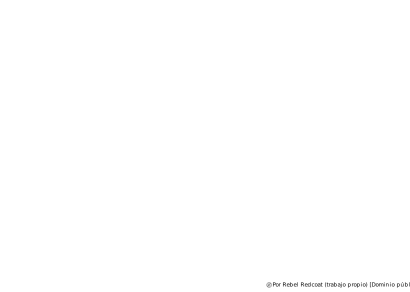
\includegraphics[width=140mm]{capitulos/img/Europe1700-14} 
	\label{fig:Europe1700} 
\end{figure}

Uno de los conceptos importantes es resaltar la transformación que experimentaron las monarquías autoritarias al convertirse en monarquías absolutas. 
Se explicarán brevemente los acontecimientos desde el año 1.517 al 1.700, ya que se corresponde al periodo en el que gobernaron los Austrias. Se dividirá el estudio en tres partes. La primera de ellas comienza en el año 1.515 y concluye en el año 1.560. Se ha de destacar que España tuvo una gran expansión geográfica y económica. Esto se debió a que se conquistaron en América los imperios azteca, maya e inca. Con posterioridad se consolidaban también las relaciones comerciales entre India y Europa. A partir de 1.535 se comenzaba a dar el fenómeno conocido como \emph{la revolución de los precios en Europa}.
La segunda etapa estuvo comprendida entre los años 1.561 y 1.660. Convendría destacar que en esa fase se produjo un fuerte enfrentamiento religioso e ideológico, destacando estos hechos:
\begin{enumerate}
	\item Europa comenzó a estar dividida por las luchas religiosas. La expansión del calvinismo frente al protestantismo fue un factor determinante para la rebelión que tuvo lugar en los Países Bajos y también las guerras de religión francesas. 
	\item Las naciones europeas recientemente constituidas se contagiaban del espíritu comercial, como era el caso de Holanda. De este modo, se convirtió en la nueva potencia comercial europea.
	\item En el año 1.600, prácticamente toda Europa sufrió una gran crisis demográfica, económica y social, que desembocó en una guerra civil: \emph{la guerra de los Treinta Años}.
\end{enumerate} 
La última etapa, abarcaría desde 1.660 hasta 1.700. Para entonces, la tulipomanía ya había sido superada por los holandeses y daba paso a las burbujas económicas que srugieron en Francia e Inglaterra. Los hechos más relevantes para el estudio de éstas fueron:
\begin{enumerate}
	\item La hegemonía española daba paso a la francesa. Además, Inglaterrá se convirtió en la primera potencia naval. 
	\item Surgió la revolución científica, con Galileo, Descartes y Newton como figuras sobresalientes. Éste último fue victima de la burbuja de la Compañía de los Mares del Sur.
\end{enumerate}

En el siguiente mapa de América del año 1.700, se puede comprobar que Francia conquistó gran parte del territorio americano. De este modo se vio favorecido el desarrollo de la burbuja económica de la Compañía de los Mares del Sur. Como se puede observar en el mapa, Francia poseía mayor porcentaje de territorios que Inglaterra y España.

\begin{figure}[!h] 
	\caption{América del norte en la primera mitad del siglo XVIII} 
	\centering
	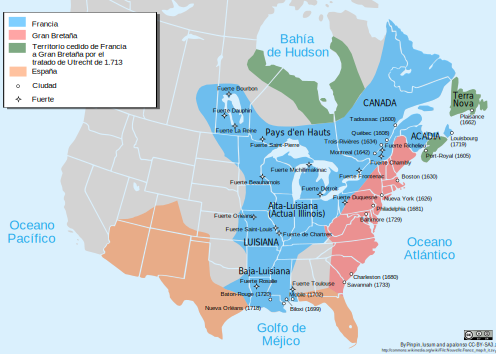
\includegraphics[width=140mm]{capitulos/img/louisiana} 
	\label{fig:louisiana} 
\end{figure}
 
Gracias a estas conquistas, el gobierno francés concedió a John Law el monopolio comercial entre Francia y las colonias de Luisiana y Canadá. Esta colonia abarcaba casi los 3.000 kilómetros de la desembocadura del río Mississippi. Incluía los actuales estados de Louisiana, Mississippi, Arkansas, Missouri, Illinois, Iowa, Wisconsin y Minnesota. Estas colonias se consideraban valiosas por su abundancia de recursos. Por ejemplo las pieles de castor y los metales preciosos de Louisiana entre otros. Aún así, como se ha podido comprobar a lo largo del capítulo tres, no era tan abundante la riqueza como se hizo creer en Francia, perdiendo así la confianza de la ciudadanía y provocando el colapso de la burbuja económica.




\end{document}
